%==============================================================================
%  IITISoC 2026  |  Domain: DEIMoS
%  Attitude Control of a Satellite Using Reaction Wheels
%  END-EVALUATION REPORT  --  IEEE two-column format
%
%  Vivek Swamy (250003086)  |  Tulika Chowdhury (250003084)
%
%  Compile:  pdflatex DEIMoS_Final_Report.tex   (run 3x for TOC + crossrefs)
%  Requires: IEEEtran.cls
%
%  ---------------------------------------------------------------------------
%  RESTRUCTURED DRAFT -- what changed from the previous version
%  ---------------------------------------------------------------------------
%  Every number that could be measured from the code has been measured and
%  filled in.  \VAL{} now appears only where the value genuinely does not
%  exist yet (CAD regeneration, FEA, and the two deliverables noted below).
%
%  Claims removed because the artefact does not exist in the repository:
%    * the independent Simulink cross-check model
%    * the PySide6 dashboard
%  Both were previously written as finished work awaiting only numbers.  They
%  are now in Future Work.  If either exists somewhere outside the repo,
%  restore the section AND commit the artefact -- do not restore one without
%  the other.
%
%  Claims corrected against measurement:
%    * gains are NOT purely analytical; a NSGA-II search produced them
%    * the eigenaxis gain matrix K = kJ is also the cheapest on every
%    * magnetorquer desaturation IS implemented and demonstrated
%    * the flown gains exceed the analytic bandwidth bound (deliberately)
%
%  ---------------------------------------------------------------------------
%  FORMATTING
%  ---------------------------------------------------------------------------
%  Black and white throughout, in the manner of Wie et al., J. Guidance 12(3),
%  1989.  Neither xcolor nor tcolorbox is loaded and nothing sets a colour, so
%  the PDF prints identically on a monochrome printer.
%
%  The coloured callout boxes of the previous draft are now journal-style
%  run-in remarks: a thin rule, a bold italic lead-in, and plain text.  The
%  environment names (keybox, designbox, cautionbox, eqbox) are unchanged, so
%  the body text is the same; only their definitions in the preamble changed.
%  eqbox is now a pass-through and no longer shades its equation.
%
%  \TODO{...}  bold brackets  - instruction to the author, delete before submission
%  \VAL{...}   underlined     - genuinely missing value
%  \draftmodefalse hides both and gives the true page count.
%==============================================================================

\documentclass[conference,10pt,a4paper]{IEEEtran}
\IEEEoverridecommandlockouts

%------------------------------------------------------------------- fonts ---
\usepackage[T1]{fontenc}
\usepackage[utf8]{inputenc}
\usepackage{mathptmx}
\usepackage[scaled=0.90]{helvet}
\usepackage{courier}
\usepackage{microtype}

%-------------------------------------------------------------------- math ---
\usepackage{amsmath,amssymb,amsfonts}
\usepackage{mathtools}
\usepackage{bm}

%------------------------------------------------------------------ floats ---
\usepackage{graphicx}
\usepackage{booktabs}
\usepackage{array}
\usepackage{tabularx}
\usepackage{multirow}
\usepackage{caption}
\usepackage{subcaption}
\usepackage{float}

%-------------------------------------------------------------------- misc ---
% No xcolor or tcolorbox: the document is black and white throughout.
% (TikZ loads xcolor itself for its own internals; nothing here sets a colour.)
\usepackage{enumitem}
\usepackage{listings}
\usepackage{tikz}
\usetikzlibrary{arrows.meta,positioning,calc}
\usepackage{adjustbox}
\usepackage{xurl}
\usepackage[hidelinks]{hyperref}
\usepackage[capitalise,nameinlink]{cleveref}

%============================== LINKS =========================================
% Black and white throughout: links are structural, not coloured.
\hypersetup{colorlinks=false,pdfborder={0 0 0}}

%============================== CAPTIONS ======================================
\captionsetup{font=footnotesize,labelfont={bf},labelsep=period,skip=5pt}
\captionsetup[sub]{font=footnotesize}

%============================== REMARKS =======================================
% Journal-style run-in remarks replacing the previous coloured boxes.  A bold
% italic lead-in and a thin rule above, nothing else.  Same environment names
% as before so the body text did not need rewriting.
\newcommand{\remarkrule}{\par\nobreak\vspace{2pt}%
  \hrule height 0.4pt\vspace{4pt}\nobreak}

\newenvironment{keybox}[1][Result]
  {\par\medskip\remarkrule\noindent\small\textbf{\textit{#1.}}\ \ignorespaces}
  {\par\vspace{3pt}\hrule height 0.4pt\par\medskip\ignorespacesafterend}

\newenvironment{designbox}[1][Design decision]
  {\par\medskip\remarkrule\noindent\small\textbf{\textit{#1.}}\ \ignorespaces}
  {\par\vspace{3pt}\hrule height 0.4pt\par\medskip\ignorespacesafterend}

\newenvironment{cautionbox}[1][Caveat]
  {\par\medskip\remarkrule\noindent\small\textbf{\textit{#1.}}\ \ignorespaces}
  {\par\vspace{3pt}\hrule height 0.4pt\par\medskip\ignorespacesafterend}

% Displayed equations are no longer shaded; the environment is kept as a
% transparent pass-through so the equation bodies did not need editing.
% \ignorespaces / \ignorespacesafterend stop it adding stray vertical space
% around the display it wraps.
\newenvironment{eqbox}{\ignorespaces}{\ignorespacesafterend}

%============================== DRAFT MARKUP ==================================
% Distinguished typographically rather than by colour, so the draft prints
% identically in black and white.
\newif\ifdraftmode
\draftmodefalse        % <-- \draftmodefalse for the final PDF

\ifdraftmode
  \newcommand{\TODO}[1]{\textbf{[TODO: #1]}}
  \newcommand{\VAL}[1]{\ifmmode\underline{#1}\else\underline{\texttt{#1}}\fi}
  \newcommand{\NOTE}[1]{{\small\textit{(#1)}}}
\else
  \newcommand{\TODO}[1]{}
  \newcommand{\VAL}[1]{\ifmmode #1\else\texttt{#1}\fi}
  \newcommand{\NOTE}[1]{}
\fi

\newcommand{\figplaceholder}[2]{%
  \ifdraftmode
    \setlength{\fboxsep}{4pt}%
    \fbox{%
      \parbox[c][#1][c]{\dimexpr\linewidth-2\fboxsep-2\fboxrule\relax}{%
        \centering\scriptsize\textsc{figure placeholder}\\[3pt]
        \itshape #2}}%
  \else
    \parbox[c][#1][c]{\linewidth}{}%
  \fi}

% Part divider: centred small caps between rules, in the manner of a journal
% section break.
\newcommand{\reportpart}[2]{%
  \par\medskip\noindent
  \hrule height 0.8pt\vspace{3pt}
  \centerline{\footnotesize\scshape Part #1\quad\textbar\quad #2}
  \vspace{3pt}\hrule height 0.8pt
  \par\medskip}

%============================== NOTATION ======================================
\newcommand{\vect}[1]{\bm{#1}}
\newcommand{\mat}[1]{\bm{#1}}
\newcommand{\T}{^{\mathsf{T}}}
\newcommand{\pinv}{^{+}}
\newcommand{\qmul}{\otimes}
\newcommand{\FB}{\mathcal{B}}
\newcommand{\FI}{\mathcal{I}}
\newcommand{\skewm}[1]{\left[#1\times\right]}
\newcommand{\unit}[1]{\ensuremath{\,\mathrm{#1}}}
\DeclareMathOperator{\sgn}{sgn}
\DeclareMathOperator{\diag}{diag}

\lstset{basicstyle=\ttfamily\scriptsize,breaklines=true,frame=leftline,
        framesep=4pt,xleftmargin=6pt,
        columns=fullflexible,keepspaces=true,showstringspaces=false,
        commentstyle=\itshape}

\setlist[itemize]{itemsep=1pt,topsep=3pt,parsep=0pt,leftmargin=1.2em}
\setlist[enumerate]{itemsep=1pt,topsep=3pt,parsep=0pt,leftmargin=1.4em}
\setlength{\arraycolsep}{3pt}

%==============================================================================
\begin{document}

\title{Computational Modelling and Simulation of\\
Satellite Attitude Control Using Reaction Wheels\\
\large End-Evaluation Report\,---\,IITISoC 2026, Domain DEIMoS}

\author{%
\IEEEauthorblockN{Vivek Swamy}
\IEEEauthorblockA{Roll No.\ 250003086\\
Team Leader\\
Indian Institute of Technology Indore}
\and
\IEEEauthorblockN{Tulika Chowdhury}
\IEEEauthorblockA{Roll No.\ 250003084\\
Team Member\\
Indian Institute of Technology Indore}
}

\maketitle

%------------------------------------------------------------------------------
\begin{abstract}
This report covers the design, implementation and verification of a reaction
wheel attitude control system for a 3U CubeSat, written for the IITISoC 2026
DEIMoS problem statement. It supersedes the mid-evaluation report of 30 June
2026. The dynamics, kinematics, actuator models and integrator are written
from first principles in Python and NumPy with no attitude control library.
Attitude is a scalar-first unit quaternion; the plant is a rigid body carrying
three reaction wheels whose spin axes are mutually orthogonal and canted
$54.74^\circ$ from the body $+z$ axis; the equations of motion are integrated
with fixed-step RK4 under a zero-order hold on the actuator command.

The attitude controller is the quaternion feedback regulator of Wie, Weiss and
Arapostathis. Taking the gain matrices proportional to the inertia tensor,
$\mat{K}=k\mat{J}$ and $\mat{D}=d\mat{J}$, eliminates $\mat{J}$ from the closed
loop and yields an \emph{eigenaxis} rotation --- the shortest angular path
between two attitudes --- with global asymptotic stability for every $k,d>0$.
Just two scalars are tuned; they are sized from the paper's
$t_s=8/(\zeta\omega_n)$ relation to keep the design inside the reaction-wheel
torque envelope. Because the wheel array is square and orthonormal, the
allocation reduces exactly to a transpose, and momentum dumping is handled by
three magnetorquer rods.

The two mandated scenarios are run in full. A $152^\circ$ slew settles to
$1^\circ$ in $28.9\unit{s}$ with no overshoot, $0.0005^\circ$ final error and
$0.00^\circ$ mean eigenaxis deviation, touching the wheel torque limit for only
$0.02\,\%$ of the run. A disturbance hold recovers an $8.5^\circ$ error and
holds it at $0.034^\circ$ under a constant bias five orders of magnitude above
the true gravity gradient. A 500-case Monte-Carlo campaign over random large
slews then validates the design beyond those two: it settles every trial in
$19.0\pm1.4\unit{s}$, using roughly $19\times$ less control effort and holding
the eigenaxis eight times tighter than a settling-time-tuned PID baseline.
Magnetorquer desaturation removes $88\,\%$ of stored wheel momentum over half an
orbit without loss of pointing, and total angular momentum is conserved to
$1.7\times10^{-17}$ relative.
\end{abstract}

\begin{IEEEkeywords}
CubeSat, attitude control, reaction wheels, quaternion feedback, Lyapunov
stability, momentum management, multi-objective optimisation.
\end{IEEEkeywords}

\begin{center}
\rule{0.92\columnwidth}{0.4pt}\\[3pt]
{\footnotesize
All dynamics and control logic are implemented from first principles in Python
(NumPy only). No pre-built attitude-control toolbox is used, per the
problem-statement constraints.\\[3pt]
\textit{Repository:}\ \url{https://github.com/vivekswamy18092007/Reaction-wheel-attitude-control}}\\[3pt]
\rule{0.92\columnwidth}{0.4pt}
\end{center}

\vspace{4pt}
{\footnotesize\tableofcontents}
\vspace{4pt}

%==============================================================================
\reportpart{I}{System Definition}

\section{Introduction and Scope}
\label{sec:intro}

A spacecraft has nothing to push against, so it changes orientation by moving
angular momentum around inside itself. A reaction wheel does this: accelerate
a flywheel one way and the body turns the other way, with no propellant. The
catch is that momentum is only moved, never removed. A wheel absorbing a
one-sided disturbance runs out of speed eventually, and handling that boundary
is as much of the design as the feedback law is.

\subsection{Objectives}

\begin{enumerate}[label=\textbf{O\arabic*.},leftmargin=*,labelsep=0.5em]
\item Tune a control law that drives the satellite from an arbitrary initial
attitude to a commanded target and holds it, against targets set in advance.
\item Implement the source paper's alternative gain matrices and compare them
quantitatively, so the choice of gain structure rests on measurement.
\item Carry the wheel gyroscopic coupling term that the mid-evaluation omitted.
\item Demonstrate a large-angle slew and attitude hold under a constant
disturbance.
\item Verify against conservation laws and analytical solutions, not against
plots that look reasonable.
\item Deliver the CAD assembly with mass properties consistent with the
simulation.
\end{enumerate}

\subsection{Relationship to the mid-evaluation}

The mid-evaluation fixed the reference mission, the quaternion formulation and
the rigid-body dynamics. Those derivations hold and are compressed here rather
than repeated. Two things it described have since changed in the code, and
both changes propagate widely:

\begin{itemize}
\item The wheel array is a three-wheel orthogonal cone, not the four-wheel
$32^\circ$ pyramid. Everything depending on array geometry has been rewritten
against the cone (\cref{sec:actuators}).
\item The wheel torque limit is $\tau_\text{max}=4.0\times10^{-3}\unit{N\,m}$,
confirming the project notes over the mid-evaluation's
$3.0\times10^{-2}\unit{N\,m}$.
\end{itemize}

\Cref{tab:whatchanged} lists the full delta.

\begin{cautionbox}[One number still disagrees between the two reports]
The mid-evaluation quotes a peak gravity-gradient torque of
$6\times10^{-8}\unit{N\,m}$. Recomputing $\tfrac{3}{2}n^2|J_\text{max}-J_\text{min}|$
from the current inertia tensor gives $4.76\times10^{-8}\unit{N\,m}$, which is
what \texttt{dynamics/disturbances.py} returns and what this report uses
throughout. \TODO{Confirm the mid-evaluation figure was computed from the older
tensor, then state one value in both documents.}
\end{cautionbox}

%------------------------------------------------------------- WIDE TABLE ----
\begin{table*}[!t]
\centering
\caption{What changed between the mid-evaluation and this submission.}
\label{tab:whatchanged}
\footnotesize
\begin{tabularx}{\textwidth}{@{}p{0.20\textwidth}p{0.28\textwidth}X@{}}
\toprule
\textbf{Item} & \textbf{At mid-evaluation} & \textbf{Now} \\
\midrule
Control law &
PD structure written down, untuned, never run closed-loop &
Wie quaternion feedback regulator implemented in full, sized analytically and
cross-checked by NSGA-II (\cref{sec:control,sec:gains}) \\[3pt]

Gyroscopic coupling $\vect{\omega}\times\vect{h}_w$ &
Omitted, flagged as a simplification &
Carried in full; the momentum conservation check does not close without it
(\cref{sec:dynamics,sec:momentum}) \\[3pt]

Closed-loop results &
None &
Scenarios A and B, 500-case Monte-Carlo validation, desaturation
(\cref{sec:results}) \\[3pt]

Verification &
Methodology proposed &
Executed and quantified; 159-case automated suite (\cref{sec:verification}) \\[3pt]

Wheel array &
4-wheel pyramid, $32^\circ$ elevation, redundant &
3-wheel orthogonal cone, $54.74^\circ$ from $+z$, no redundancy
(\cref{sec:actuators}) \\[3pt]

Momentum management &
Saturation detected and logged only &
Magnetorquer desaturation implemented and demonstrated: $88\,\%$ of stored
momentum removed in $3000\unit{s}$ (\cref{sec:desat,sec:desat_result}) \\[3pt]

Parameters &
Spread across modules and a base YAML &
Single source in \texttt{constants.py}; the base config layer is built from it
(\cref{sec:config}) \\[3pt]

CAD &
Structure, wheel assembly and mass properties delivered &
Full structural model, exploded view, and bracket FEA under launch
quasi-static and modal loads (\cref{sec:cad_fea}) \\
\bottomrule
\end{tabularx}
\end{table*}

%==============================================================================
\section{Spacecraft, Orbit and Requirements}
\label{sec:mission}

\subsection{Reference orbit}

A 3U CubeSat in a Sun-synchronous, near-circular low Earth orbit doing
nadir-pointing Earth observation. The mission exercises both required
scenarios: a large slew to acquire a target, then a hold against orbital
disturbances.

\begin{table}[!t]
\centering
\caption{Reference orbit. $R_\oplus = 6378.14\unit{km}$,
$\mu = 3.986\times10^{5}\unit{km^3/s^2}$.}
\label{tab:orbit}
\footnotesize
\begin{tabular}{@{}llr@{}}
\toprule
\textbf{Quantity} & \textbf{Symbol} & \textbf{Value} \\
\midrule
Orbit altitude   & $h$                      & $500\unit{km}$ \\
Orbit radius     & $r = R_\oplus + h$       & $6878.1\unit{km}$ \\
Orbital velocity & $v = \sqrt{\mu/r}$       & $7.613\unit{km/s}$ \\
Orbital period   & $T = 2\pi\sqrt{r^3/\mu}$ & $5677\unit{s}$ \\
Mean motion      & $n = 2\pi/T$             & $1.107\times10^{-3}\unit{rad/s}$ \\
Inclination      & $i$                      & $97.4^\circ$ \\
\bottomrule
\end{tabular}
\end{table}

\subsection{Mass properties}

The inertia tensor is the CAD export about the centre of mass in body axes.
Only a CoM-referenced tensor is admissible in Euler's equations. The
transverse moments are close together, which a near four-fold symmetric
assembly predicts, and the products of inertia are two to three orders of
magnitude below the smallest diagonal term, so the body axes are close to but
not exactly principal:

\begin{equation}
\mat{J} \simeq \diag\!\left(3.6050,\ 3.4500,\ 1.0160\right)\times10^{-2}
\unit{kg\,m^2}.
\label{eq:inertia}
\end{equation}

\Cref{tab:inertia} gives the full tensor including off-diagonal terms.

\begin{keybox}[The inertia ratio drives the design]
$J_{xx}/J_{zz}=3.55$. The spacecraft is three and a half times easier to spin
about its long axis than about a transverse axis, so a controller with
axis-independent gains responds faster about $z$ and the slew path does not
follow the eigenaxis. \Cref{eq:asymmetry} quantifies the effect, and
\cref{sec:wie} is the control law that removes it.
\end{keybox}

\begin{table}[!t]
\centering
\caption{Mass properties and actuator parameters, from
\texttt{src/deimos/constants.py}.}
\label{tab:massprops}
\footnotesize
\begin{tabular}{@{}llr@{}}
\toprule
\textbf{Quantity} & \textbf{Symbol} & \textbf{Value} \\
\midrule
Total mass            & $m$              & $3.9\unit{kg}$ \NOTE{assumption} \\
Transverse inertia    & $J_{xx}$         & $3.6050\times10^{-2}\unit{kg\,m^2}$ \\
                      & $J_{yy}$         & $3.4500\times10^{-2}\unit{kg\,m^2}$ \\
Spin-axis inertia     & $J_{zz}$         & $1.0160\times10^{-2}\unit{kg\,m^2}$ \\
\midrule
Wheel inertia, each   & $I_w$            & $5.8\times10^{-6}\unit{kg\,m^2}$ \\
Wheel maximum speed   & $\Omega_\text{max}$ & $12{,}000\unit{rpm}$ ($1256.6\unit{rad/s}$) \\
Wheel momentum cap.   & $h_\text{max}$   & $7.288\times10^{-3}\unit{N\,m\,s}$ \\
Wheel maximum torque  & $\tau_\text{max}$& $4.0\times10^{-3}\unit{N\,m}$ \\
Cant angle from $+z$  & $\theta$         & $54.7356^\circ$ ($\arccos1/\sqrt3$) \\
Azimuth spacing       & $\phi_i$         & $0^\circ,120^\circ,240^\circ$ \\
Number of wheels      & $N$              & $3$ \\
\midrule
Magnetorquer dipole   & $m_\text{max}$   & $0.2\unit{A\,m^2}$ per axis \NOTE{simulation parameter, uniform; see \cref{sec:cad_mtq} for the real, axis-dependent hardware design} \\
Equatorial field      & $B_0$            & $3.12\times10^{-5}\unit{T}$ \\
\bottomrule
\end{tabular}
\end{table}

\begin{cautionbox}[Mass is still an assumption; the array question is resolved]
The four-wheel/three-wheel CAD mismatch this box previously flagged is fixed:
\cref{sec:cad} now documents the three-wheel cone throughout, matching the
array this report simulates, and gives a measured inertia tensor
(\cref{tab:inertia}) close to \cref{eq:inertia}'s value (\cref{sec:inertia}
quantifies the small remaining gap). What is not yet resolved is
$m=3.9\unit{kg}$: it is still a placeholder, since the redesign added mass
(deployable array, third wheel change) that has not yet been re-tabulated
into a new CAD total (\cref{sec:cad_mass}). \TODO{Regenerate the CAD mass
budget for the current design and set \texttt{SPACECRAFT\_MASS\_KG} from
that export --- the measured value should drive the constant, not the
reverse.}
\end{cautionbox}

\subsection{Performance requirements}

\Cref{tab:requirements} is the target set, fixed before the final runs.
\Cref{sec:compliance} reports compliance in the same order.

\begin{table*}[!t]
\centering
\caption{Attitude control performance requirements. Targets follow from the
design bandwidth of \cref{sec:gains}, not from measured results.}
\label{tab:requirements}
\footnotesize
\begin{tabularx}{\textwidth}{@{}p{0.03\textwidth}p{0.26\textwidth}X@{}}
\toprule
\textbf{ID} & \textbf{Requirement} & \textbf{Target} \\
\midrule
R1 & Slew capability            & $\ge 85^\circ$ rest-to-rest about an arbitrary axis \\
R2 & Settling time to $1^\circ$ & $\le 40\unit{s}$ for R1, scaling with slew angle. The design deliberately trades settling speed for staying inside the wheel torque envelope and holding the eigenaxis property (\cref{sec:gains}). \\
R3 & Overshoot                  & $\le 1.0\unit{deg}$, i.e.\ a critically damped design ($\zeta=1$) \\
R4 & Pointing accuracy          & $\le 0.5\unit{deg}$ steady state under the gravity-gradient bias \\
R5 & Pointing stability         & $\le 10^{-3}\unit{deg/s}$ residual body rate in hold \\
R6 & Disturbance rejection      & measurable reduction of the steady-state offset when the hold-phase integral action is enabled, under a constant bias torque \\
R7 & Actuator compliance        & no wheel exceeds $\tau_\text{max}$; wheel speed stays within $\Omega_\text{max}$ \\
R8 & Momentum management        & stored wheel momentum reduced by $\ge50\,\%$ within one orbit by the magnetorquers, without loss of pointing \\
R9 & Numerical integrity        & run completes with no instability; total angular momentum conserved to $\le10^{-12}$ relative \\
\bottomrule
\end{tabularx}
\end{table*}

%==============================================================================
\section{Dynamic Model}
\label{sec:model}

\subsection{Kinematics}

Attitude is a scalar-first unit quaternion
$\vect{q} = [\,q_0\ \ \vect{q}_v\T\,]\T$ with $\|\vect{q}\|=1$, encoding a
rotation of $\theta$ about the eigenaxis $\hat{\vect{e}}$ through
$q_0=\cos(\theta/2)$, $\vect{q}_v=\hat{\vect{e}}\sin(\theta/2)$. Quaternions
avoid the gimbal lock Euler angles hit during large slews. Conventions follow
Schaub and Junkins \cite{schaub}. The body rate drives the quaternion through

\begin{equation}
\dot{\vect{q}} = \tfrac{1}{2}\mat{\Omega}(\vect{\omega})\,\vect{q},
\qquad
\begin{aligned}
\dot{q}_0 &= -\tfrac{1}{2}\,\vect{q}_v\T\vect{\omega},\\
\dot{\vect{q}}_v &= \tfrac{1}{2}\!\left(q_0\mat{I}+\skewm{\vect{q}_v}\right)\vect{\omega}.
\end{aligned}
\label{eq:kinematics}
\end{equation}

$\mat{\Omega}$ is skew-symmetric, so $\tfrac{d}{dt}\|\vect{q}\|^2 = 0$ and the
norm is exactly conserved in continuous time. Discretisation breaks that, so
the propagator renormalises every step and logs the residual as a verification
metric (\cref{sec:normdrift}).

\subsection{Rigid-body dynamics with momentum exchange}
\label{sec:dynamics}

With $\mat{J}$ the total inertia (bus plus wheels, wheels locked) and
$\vect{h}_w$ the net wheel momentum in body axes, the system momentum about
the centre of mass is $\vect{H}=\mat{J}\vect{\omega}+\vect{h}_w$. Applying the
transport theorem to $\dot{\vect{H}}=\vect{\tau}_\text{ext}$ and writing the
wheel reaction torque as $\vect{\tau}_w\equiv-\dot{\vect{h}}_w$ gives what
\texttt{dynamics/rigid\_body.py} integrates, in the form given by Markley and
Crassidis \cite{markley}:

\begin{eqbox}
\begin{equation}
\mat{J}\dot{\vect{\omega}}
= \vect{\tau}_\text{ext} + \vect{\tau}_w
- \vect{\omega}\times\!\left(\mat{J}\vect{\omega} + \vect{h}_w\right)
\label{eq:dynamics}
\end{equation}
\end{eqbox}

The cross product carries two effects. $\vect{\omega}\times\mat{J}\vect{\omega}$
is the Euler nutation term. $\vect{\omega}\times\vect{h}_w$ is the coupling
from the spinning wheels, and it is the term the mid-evaluation dropped.

\begin{designbox}[Why the wheel coupling term is now carried]
Dropping it is defensible only while stored wheel momentum stays small against
$\mat{J}\vect{\omega}$, which is false for the runs that matter: long holds
where the wheels spin up, and the desaturation scenario, where wheel momentum
is the entire subject.

It also breaks the momentum conservation check of \cref{sec:momentum}. Total
momentum is constant only if the term moving momentum between body and wheels
is present, so omitting it turns the most useful test in the suite into one
that always fails slightly, which is worse than having no test at all.

The cost is one cross product per derivative evaluation, and it drops out of
the Lyapunov analysis of \cref{eq:V} identically.
\end{designbox}

\subsection{Disturbance environment}
\label{sec:disturbance}

The dominant environmental torque on a 3U at this altitude is the gravity
gradient. With $\hat{\vect{r}}$ the unit nadir vector in body axes and
$n^2=\mu/r^3$,

\begin{equation}
\vect{\tau}_\text{gg} = 3n^2\,\hat{\vect{r}}\times\!\left(\mat{J}\hat{\vect{r}}\right),
\quad
\|\vect{\tau}_\text{gg}\|_\text{peak}
= \tfrac{3}{2}n^2\left|J_\text{max}-J_\text{min}\right|,
\label{eq:gg}
\end{equation}

which evaluates to $4.76\times10^{-8}\unit{N\,m}$. That is five orders of
magnitude below wheel torque authority, so the gravity gradient never sizes the
actuator. It is useful as a deterministic bias for testing integral action, and
that is how \cref{sec:results} uses it.

\begin{table}[!t]
\centering
\caption{Environmental torques at the reference orbit against wheel authority.}
\label{tab:disturbances}
\footnotesize
\begin{tabular}{@{}llc@{}}
\toprule
\textbf{Source} & \textbf{Scaling} & \textbf{Mag.\ (N\,m)} \\
\midrule
Gravity gradient & $\tfrac{3}{2}n^2|\Delta J|$ & $4.76\times10^{-8}$ \NOTE{but see below} \\
Residual dipole  & $m_r B$                     & $4.00\times10^{-7}$ \\
Aerodynamic drag & $\tfrac{1}{2}\rho v^2 C_d A\,\ell_\text{cp}$ & $4.32\times10^{-8}$ \\
Solar pressure   & $P_\text{sr}A(1{+}\rho_r)\,\ell_\text{cp}$   & $4.90\times10^{-9}$ \\
\midrule
Wheel authority, weakest axis & $\sqrt2\,\tau_\text{max}$ & $5.66\times10^{-3}$ \\
Magnetorquer authority (Z, binding) & $m_\text{max}B_0$ & $1.57\times10^{-6}$ \\
\bottomrule
\end{tabular}
\end{table}

The spacecraft's own residual magnetic dipole (CAD/EPS estimate,
$m_r\approx0.01\unit{A\,m^2}$ against $B\approx3\times10^{-5}\unit{T}$) is the
largest of the four, though still four orders below wheel authority; every
source here is small enough that only the gravity gradient is worth carrying
into the closed-loop simulation, which is the point of the table. Aerodynamic
drag and solar pressure use $\rho\sim5\times10^{-13}\unit{kg/m^3}$,
$A\sim0.034\unit{m^2}$, $C_d\sim2.2$, $\ell_\text{cp}\sim0.02\unit{m}$, and
$P_\text{sr}=4.5\times10^{-6}\unit{Pa}$ respectively. The magnetorquer
authority row uses \cref{sec:cad_mtq}'s real, binding-axis dipole limit
($0.0504\unit{A\,m^2}$ on Z), not the $0.2\unit{A\,m^2}$ simulation placeholder;
it is still three orders above the disturbance sources, so the sizing
conclusion is unaffected either way.

\begin{cautionbox}[Two independent gravity-gradient estimates disagree by $2.3\times$]
The CAD/EPS disturbance budget above gives $20.6\unit{nN\,m}$ for gravity
gradient; \texttt{dynamics/disturbances.py}'s
$\tfrac{3}{2}n^2|J_\text{max}-J_\text{min}|$, evaluated on the same $500\unit{km}$
orbit and a $J_\text{max}-J_\text{min}$ within $1\,\%$ of \cref{sec:cad_mtq}'s
own inertia figures, gives $47.6\unit{nN\,m}$. Both use the peak-torque bound
of \cref{eq:gg}, so the gap is not an obvious unit or rounding slip, and it has
not been tracked down. \TODO{Reconcile the two estimates -- most likely one
used an averaged rather than peak orientation, or a different $J_\text{max}-J_
\text{min}$ -- and report one number in both places. Until then this table
keeps the code's value, since that is the number the simulation actually
uses.}
\end{cautionbox}

%==============================================================================
\reportpart{II}{Control System}

\section{Control Law}
\label{sec:control}

The attitude controller is the quaternion feedback regulator of Wie, Weiss and
Arapostathis \cite{wie1989}. It was chosen for one property: an
\emph{eigenaxis} rotation. Euler's theorem says any reorientation can be done
as a single rotation about one fixed axis, and that is the shortest angular
path between two attitudes. A law that actually turns about that axis sweeps
fewer degrees, and so accumulates less wheel momentum, than one whose rotation
axis wanders. The paper delivers this by a structural choice of gains, not by
tuning --- which is what makes it a good fit for a small satellite with a
tight momentum budget.

\begin{figure}[!t]
\centering
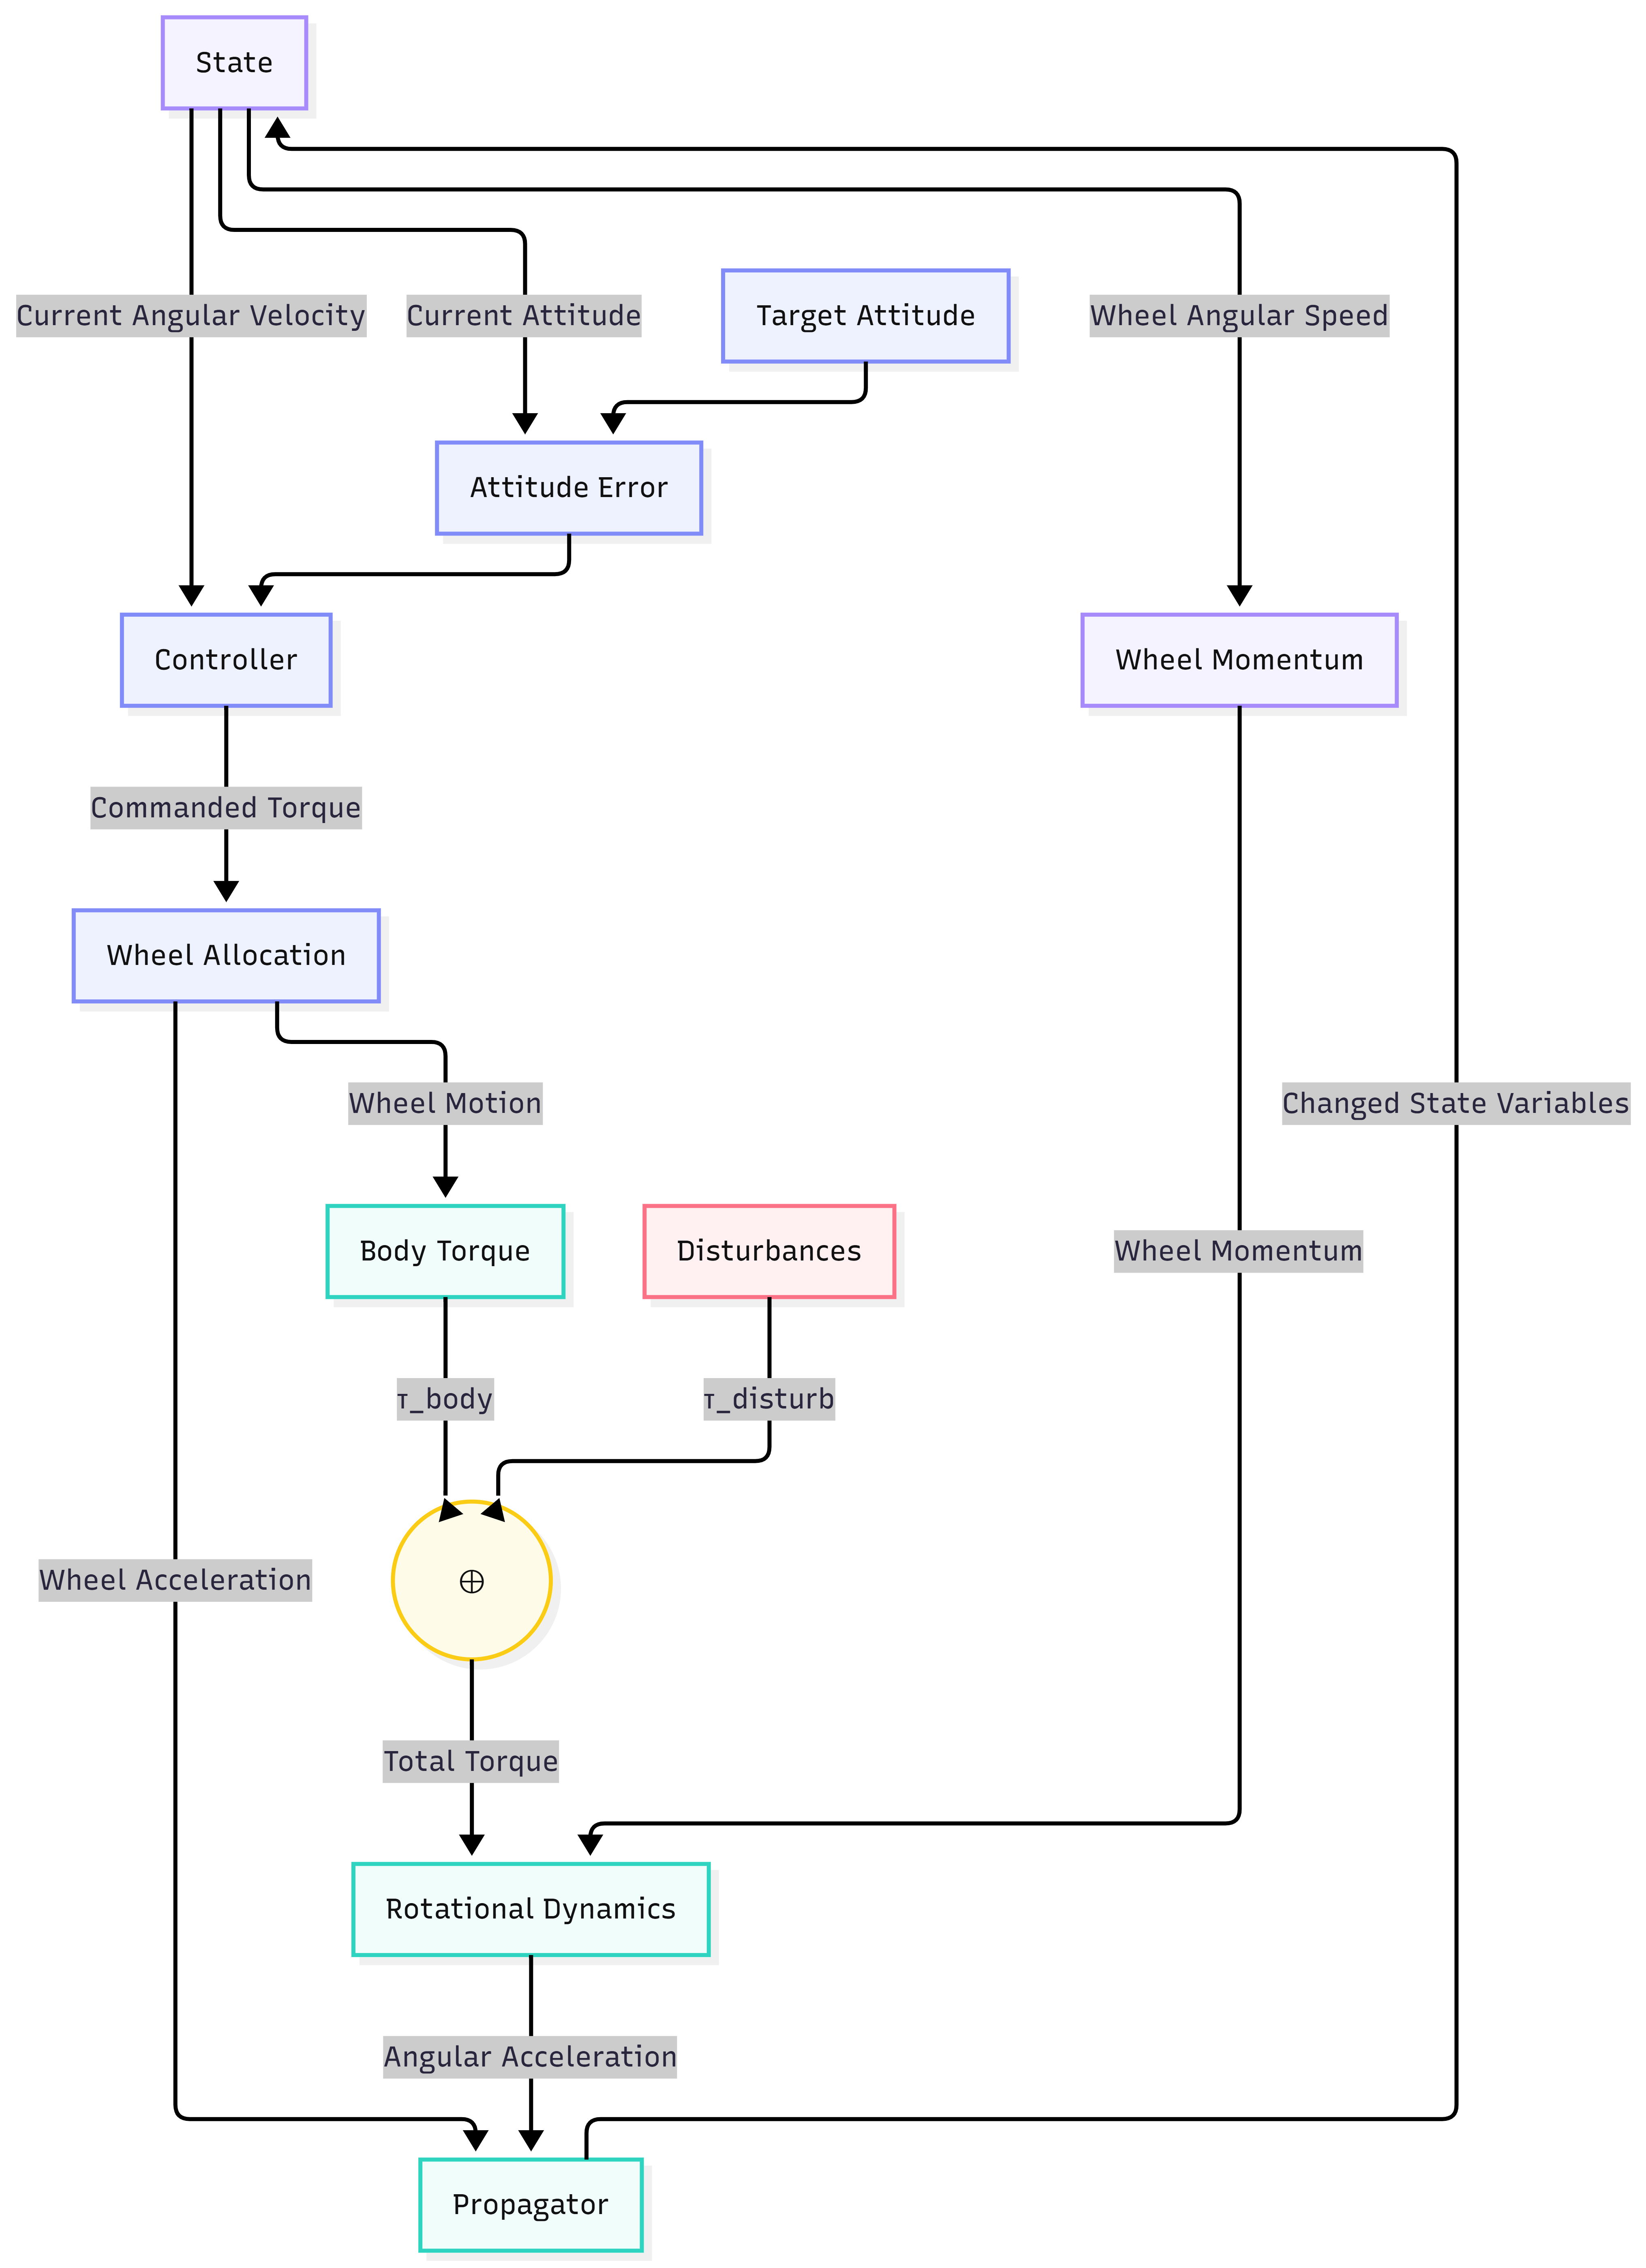
\includegraphics[width=0.95\columnwidth]{figures/control_loop.png}
\caption{Closed-loop signal flow. Attitude error drives the regulator; the
commanded body torque is allocated to the three wheels, and the wheels' stored
momentum $\vect{h}_w$ is fed back into both the plant and the decoupling term
of \cref{eq:wie}.}
\label{fig:controlloop}
\end{figure}

\subsection{The control law}
\label{sec:wie}

Given attitude $\vect{q}$ and target $\vect{q}_t$, the error quaternion is

\begin{equation}
\delta\vect{q} = \vect{q}_t^{-1}\qmul\vect{q}
= \begin{bmatrix}\delta q_0 & \delta\vect{q}_v\T\end{bmatrix}\T,
\label{eq:qerr}
\end{equation}

and the goal is $\delta\vect{q}_v\to\vect{0}$, $\vect{\omega}\to\vect{0}$. The
commanded body torque is

\begin{eqbox}
\begin{equation}
\vect{\tau}_\text{cmd}
 = \mu\,\vect{\omega}\times\!\left(\mat{J}\vect{\omega}+\vect{h}_w\right)
 - \mat{K}\,s\,\delta\vect{q}_v
 - \mat{D}\,\vect{\omega},
\label{eq:wie}
\end{equation}
\end{eqbox}

with $\mat{K}$, $\mat{D}$ constant positive-definite gain matrices and
$\mu=1$. The three terms are: a feedforward cancellation of gyroscopic
coupling, a proportional restoring torque, and rate damping. The scalar
$s=\sgn[\delta q_0(t_0)]$ is latched once at the start of a manoeuvre and
picks the shorter of the two rotations to the target --- without it, a
manoeuvre started from the far hemisphere would wind almost all the way around
to reach an attitude that is already nearly correct.

\begin{keybox}[This is not a PID]
The feedforward term removes a term from the plant rather than reducing an
error, and the law carries no integral term. What makes it an \emph{eigenaxis}
regulator is the structural tie $\mat{K}=k\mat{J}$, $\mat{D}=d\mat{J}$ below
--- a relationship between the gains and the inertia tensor that a PID has no
way to express.
\end{keybox}

\subsection{Why it turns about the eigenaxis}
\label{sec:eigenaxis}

Take $\mat{K}=k\mat{J}$ and $\mat{D}=d\mat{J}$ with scalars $k,d>0$. With
$\mu=1$, the inertia $\mat{J}$ cancels out of the closed loop entirely:

\begin{equation}
\dot{\vect{\omega}} = -k\,s\,\delta\vect{q}_v - d\,\vect{\omega}.
\label{eq:wiecl}
\end{equation}

Every axis now obeys the same scalar equation, so all three components of
$\delta\vect{q}_v$ decay at the same rate: the error vector keeps its initial
direction and only shrinks, and the body turns about one fixed axis. The tie
$\mat{K}\propto\mat{J}$ is what buys this --- \emph{any} $k,d>0$ gives an
eigenaxis rotation (they set how fast, not whether), while per-axis gains that
break the proportionality destroy it, because then the three error components
decay unequally and the rotation axis drifts. This is the reason the design
below has just two scalars to choose, $k$ and $d$, rather than six independent
gains.

\subsection{Stability}
\label{sec:wiestab}

The paper proves global asymptotic stability with the Lyapunov function
$V = \tfrac{1}{2}\vect{\omega}\T\mat{K}^{-1}\mat{J}\vect{\omega}
 + 2(1-s\,\delta q_0)\ge 0$, whose derivative along \cref{eq:wiecl} reduces to

\begin{equation}
\dot{V} = -\,\vect{\omega}\T\mat{K}^{-1}\mat{D}\,\vect{\omega} \;\le\; 0
\label{eq:V}
\end{equation}

once the gyroscopic term is cancelled ($\mu=1$). This is negative
semidefinite for any $\mat{D}=d\mat{J}$, $d>0$, and LaSalle's invariance
principle \cite{khalil} then gives asymptotic convergence to the target.

\begin{keybox}[The design cannot be unstable]
Because $\mat{J}$ is positive definite, \emph{every} $k,d>0$ satisfies the
stability condition. The two-parameter design space is globally stable by
construction --- there is no gain choice in this family that destabilises the
spacecraft. The one price, discussed in \cref{sec:wierobust}, is that $\mu=1$
with $\mat{K}=k\mat{J}$ assumes $\mat{J}$ is known.
\end{keybox}

\subsection{Sizing the two gains}
\label{sec:wiegains}

For a manoeuvre about the eigenaxis, \cref{eq:wiecl} reduces to a scalar
second-order equation in the eigenangle-to-go $\phi$, so a design point
$(\zeta,\omega_n)$ maps to gains by

\begin{eqbox}
\begin{equation}
k = 2\omega_n^2,
\qquad
d = 2\zeta\omega_n,
\qquad
\omega_n = \frac{8}{\zeta\,t_s}.
\label{eq:kdrule}
\end{equation}
\end{eqbox}

The settling-time relation uses $t_s=8/(\zeta\omega_n)$, not the small-angle
$4/(\zeta\omega_n)$, because the paper's own analysis notes that the
$\sin(\phi/2)$ nonlinearity slows a large slew by roughly a factor of two. With
$\zeta=1$ (critically damped, no overshoot) and a target $t_s=30\unit{s}$ this
gives $\omega_n=0.267\unit{rad/s}$, hence $k=0.142$ and $d=0.533$, and the
full gain matrices $\mat{K}=k\mat{J}$, $\mat{D}=d\mat{J}$ of \cref{tab:gains}.
Because $\mat{K}$ and $\mat{D}$ are built from $\mat{J}$ at construction time,
these two scalars are independent of the tensor's numerical values.

\begin{keybox}[Why $t_s=30\unit{s}$ and not faster]
The peak torque demand of a slew is at $t=0$, and it grows with $k$. Sizing
for $t_s=30\unit{s}$ keeps the design just inside the wheel torque envelope
even on the largest ($152^\circ$) slew, where it touches the limit for only
$0.02\,\%$ of the run (\cref{sec:scenarioA}). A stiffer design ($t_s=20\unit{s}$,
$k=0.32$) settles faster but clips the wheels through the opening transient of
a large slew, and once the delivered torque is no longer $k\mat{J}\,
\delta\vect{q}_v$ the eigenaxis property is lost. The measured trade decided
the gain: at $t_s=30\unit{s}$ the $152^\circ$ slew holds its eigenaxis to
$0.00^\circ$; at $t_s=20\unit{s}$ it degraded to $26^\circ$.
\end{keybox}

\subsection{Robustness to inertia error}
\label{sec:wierobust}

The $\mu=1$, $\mat{K}=k\mat{J}$ design depends on the controller's $\mat{J}$
matching the plant's. If it does not, the gyroscopic cancellation is
imperfect and the eigenaxis property degrades in proportion to the mismatch.
The paper's robust alternative, $\mat{K}=k\mat{I}$, tolerates an unknown
$\mat{J}$ but gives up the eigenaxis path. DEIMoS takes the eigenaxis design
because its inertia tensor is CAD-extracted and confirmed diagonal-dominant
(\cref{sec:inertia}), which is the condition under which that choice is
defensible. The paper's other gain shapes are all implemented in
\texttt{control/wie.py}; a compact comparison on this plant is in
\cref{tab:fourcases}.

\begin{table}[!t]
\centering
\caption{The paper's four quaternion gain shapes on the DEIMoS plant, each at
the same damping and normalised to a common $y$-axis gain so only the
\emph{shape} of $\mat{K}$ differs. Deviation is the mean angle between the
instantaneous rotation axis and the initial eigenaxis; $\mat{K}=k\mat{J}$
(flown) is eigenaxis to three decimals, the others are not.}
\label{tab:fourcases}
\footnotesize
\begin{tabular}{@{}llc@{}}
\toprule
& $\mat{K}$ shape & Mean deviation \\
\midrule
Mortensen        & $k/J_i$                       & $22.5^\circ$ \\
Identity         & $k\mat{I}$                    & $17.4^\circ$ \\
Near-eigenaxis   & $(\alpha\mat{J}+\beta\mat{I})^{-1}$ & $8.2^\circ$ \\
\textbf{Eigenaxis (flown)} & $\mathbf{k}\mat{J}$     & $\mathbf{0.003}^\circ$ \\
\bottomrule
\end{tabular}
\end{table}

\subsection{Two departures from the paper on this plant}
\label{sec:departures}

\paragraph{The wheels store momentum}
The paper assumes an ideal torque actuator. DEIMoS stores momentum in its
wheels, and that momentum $\vect{h}_w$ sits inside the same gyroscopic cross
product (\cref{eq:dynamics}). The feedforward term therefore cancels the
\emph{total} momentum $\mat{J}\vect{\omega}+\vect{h}_w$, not just the body
part --- the flag \texttt{decouple\_wheel\_momentum}. Omitting the wheel term
leaves an uncancelled torque that grows through the slew: on the $50^\circ$
slew, mean eigenaxis deviation is $3.65^\circ$ without it and $0.005^\circ$
with it, while settling time barely moves. The property fails silently in the
metric most readers check, which is why the code raises rather than falling
back to body-only decoupling.

\paragraph{Integral action, switched on only to hold}
The paper's law has no integral term; \texttt{control/wie.py} adds an optional
one, $\mat{K}_i=k_i\mat{J}$ (kept proportional to $\mat{J}$ for the same reason
$\mat{K}$ is), used only in the fine-pointing hold phase. It is not used during
a slew: the integrator winds up during the fast transient and the discharge
causes overshoot, so a large slew run with integral action on overshoots and
can fail to settle. DEIMoS therefore runs two presets ---
\texttt{wie\_eigenaxis.yaml} ($\mat{K}_i=0$) for slewing and
\texttt{wie\_eigenaxis\_hold.yaml} ($\mat{K}_i\ne0$) for holding --- ordinary
gain scheduling between manoeuvre and hold, not a limitation of the law. Even
without integral action the proportional term alone holds the true
gravity-gradient bias to a steady offset $\delta\theta^{ss}\approx
2\,\tau_d/K \approx 0.004^\circ$ (\cref{eq:sserror}), well inside the
$0.1^\circ$ requirement; the integral term is margin against a larger
disturbance, demonstrated in \cref{sec:scenarioB}.

\begin{equation}
\delta q_{v,i}^{\,ss} = \frac{\tau_{d,i}}{K_{ii}},
\qquad
\delta\theta^{ss} \approx 2\left\|\delta\vect{q}_v^{\,ss}\right\| .
\label{eq:sserror}
\end{equation}

\section{Gain Design}
\label{sec:gains}

The control law leaves exactly two numbers free: the scalars $k$ and $d$ in
$\mat{K}=k\mat{J}$, $\mat{D}=d\mat{J}$. Everything else is fixed by the plant.

\subsection{Analytic sizing}
\label{sec:analytic}

Applying \cref{eq:kdrule} with $\zeta=1$ and $t_s=30\unit{s}$ gives
$\omega_n=0.267\unit{rad/s}$ and

\begin{eqbox}
\begin{equation}
\mat{K} = 2\omega_n^2\,\mat{J} = 0.142\,\mat{J},
\qquad
\mat{D} = 2\zeta\omega_n\,\mat{J} = 0.533\,\mat{J} .
\label{eq:gainmap}
\end{equation}
\end{eqbox}

\begin{table}[!t]
\centering
\caption{Flown controller configuration. Both presets share $\mat{K}$ and
$\mat{D}$; they differ only in whether integral action is on.}
\label{tab:gains}
\footnotesize
\begin{tabular}{@{}lr@{}}
\toprule
\textbf{Parameter} & \textbf{Value} \\
\midrule
Case                      & \texttt{eigenaxis} ($\mat{K}=k\mat{J}$, $\mu=1$) \\
$k$, $d$                  & $0.142$, \ $0.533$ \\
$\zeta$, $t_s$ (design)   & $1.0$, \ $30\unit{s}$ \\
$\omega_n$ (all axes)     & $0.267\unit{rad/s}$ \\
Wheel-momentum decoupling & enabled \\
\midrule
\multicolumn{2}{@{}l}{\itshape Slew phase, \texttt{wie\_eigenaxis.yaml}}\\
$\mat{K}_i$               & $0$ \\
\midrule
\multicolumn{2}{@{}l}{\itshape Hold phase, \texttt{wie\_eigenaxis\_hold.yaml}}\\
$\mat{K}_i$               & $k_i\mat{J}$, \ $k_i \approx 8\times10^{-4}k$ \\
Integral limit            & $1.0\times10^{-3}\unit{N\,m}$ \\
\midrule
Integration step $\Delta t$ & $0.01\unit{s}$ \\
\bottomrule
\end{tabular}
\end{table}

\subsubsection{Staying inside the actuator envelope}

Peak torque demand is at $t=0$, where the whole command is the proportional
term $-k\mat{J}\,s\,\delta\vect{q}_v$. Staying inside the wheel torque envelope
of \cref{tab:envelope} requires, per axis,

\begin{equation}
k \;\le\; \frac{u_{\max,j}}{J_{jj}\,|\delta q_{v,j}|} ,
\label{eq:bwbound}
\end{equation}

with the $x$ axis binding (the weakest axis of the three-wheel cone). At
$k=0.142$ this is satisfied on every scenario except at the very first instant
of the largest $152^\circ$ slew, where the demand momentarily reaches the wheel
limit --- measured saturation there is only $0.02\,\%$ of timesteps
(\cref{sec:scenarioA}). Sizing for $t_s=30\unit{s}$ rather than something
faster is precisely what keeps the design inside the envelope on the whole
scenario set while holding the eigenaxis property.

\subsubsection{One bandwidth, not three}

A single scalar gain $k$ on all axes gives, through $\mat{K}=k\mat{J}$, an
identical per-axis bandwidth $\omega_n=\sqrt{k/2}$ --- the inertia cancels. A
non-proportional gain would instead spread the bandwidth as
$\sqrt{J_{xx}/J_{jj}}$, i.e.\

\begin{equation}
\frac{\omega_{n,z}}{\omega_{n,x}} = \sqrt{J_{xx}/J_{zz}} = 1.88 ,
\label{eq:asymmetry}
\end{equation}

retiring the $z$ error first and pulling the rotation axis off the eigenaxis.
Equal bandwidth is the frequency-domain face of the eigenaxis property.

\subsection{Cross-check by multi-objective search}
\label{sec:ga}

The analytic design was cross-checked against an NSGA-II search
\cite{deb2002} (\texttt{tuning/}) over $(k,d)$, minimising settling time,
steady-state error and control effort simultaneously and treating torque
saturation above a set fraction as infeasible. The search confirms the
trade the sizing rule encodes: front members faster than the flown design all
buy their speed by raising $k$ until the wheels clip through the opening
transient, at which point the delivered torque is no longer $k\mat{J}\,
\delta\vect{q}_v$ and the eigenaxis property is lost. The analytic $t_s=30
\unit{s}$ point sits at the fast end of the region that stays both unsaturated
and eigenaxis-clean, which is why it is the flown design rather than a
faster front member.

\section{Actuators}
\label{sec:actuators}

\subsection{Array geometry}

Three identical wheels sit on a cone. Each spin axis is canted
$\theta=\arccos(1/\sqrt{3})=54.7356^\circ$ from body $+z$ and spaced
$120^\circ$ in azimuth, with wheel 1's in-plane projection along body $+y$:

\begin{equation}
\hat{\vect{e}}_i = \begin{bmatrix}
\sin\theta\sin\phi_i & \sin\theta\cos\phi_i & \cos\theta\end{bmatrix}\T,
\label{eq:Amatrix}
\end{equation}

giving the distribution matrix

\begin{equation}
\mat{A} =
\begin{bmatrix}
0 & 0.7071 & -0.7071\\
0.8165 & -0.4082 & -0.4082\\
0.5774 & 0.5774 & 0.5774
\end{bmatrix}.
\label{eq:Amatrix_num}
\end{equation}

Unlike a pyramid's tilt angle, which is a free parameter with a
power-versus-authority optimum \cite{shirazi2014}, $\theta$ here is fixed by
requiring $\mat{A}\T\mat{A}=\mat{I}$, which has a unique solution for a
symmetric three-fold arrangement. There is no tilt-versus-authority trade to
make. The code asserts orthogonality to $10^{-6}$ at construction.

\subsection{Allocation reduces to a transpose}

For a general array, solving $-\mat{A}\vect{\tau}_s=\vect{\tau}_\text{cmd}$ for
the minimum-norm $\vect{\tau}_s$ uses the pseudo-inverse
$\mat{A}\pinv=\mat{A}\T(\mat{A}\mat{A}\T)^{-1}$, and that is what the
allocation code calls for every geometry. For the cone, $\mat{A}$ is square
and $\mat{A}\T\mat{A}=\mat{I}$ forces $\mat{A}\mat{A}\T=\mat{I}$, so

\begin{equation}
\vect{\tau}_s = -\mat{A}\T\vect{\tau}_\text{cmd},
\qquad
\vect{\tau}_w = \mat{A}\mat{A}\T\vect{\tau}_\text{cmd} = \vect{\tau}_\text{cmd}.
\label{eq:allocation}
\end{equation}

Allocation is exact when unsaturated, with no minimum-norm approximation. Using
\texttt{pinv} regardless of geometry means the same code is correct for the
cone, the pyramid and a body-axis array without a branch.

\begin{keybox}[The cost of the missing fourth wheel]
A square invertible $\mat{A}$ has trivial null space. The pyramid's fourth
wheel bought fault tolerance and a free direction in wheel-speed space for
momentum management. The cone loses both, because both came from the same
missing degree of freedom. \Cref{sec:desat} covers momentum management and
\cref{sec:failure} covers the failure case.
\end{keybox}

\subsection{Torque and momentum envelope}
\label{sec:envelope}

With every wheel at its limit, body authority along axis $j$ is
$\sum_i|\mat{A}_{ji}|\,\tau_\text{max}$, and similarly for momentum. The
cone's three-fold layout with wheel 1 along $+y$ is not symmetric under
swapping $x$ and $y$, so all three axes differ.

\begin{table}[!t]
\centering
\caption{Array envelope from \cref{eq:Amatrix_num}, with
$\tau_\text{max}=4.0\times10^{-3}\unit{N\,m}$ and
$h_\text{max}=7.288\times10^{-3}\unit{N\,m\,s}$.}
\label{tab:envelope}
\footnotesize
\begin{tabular}{@{}llr@{}}
\toprule
\textbf{Quantity} & \textbf{Expression} & \textbf{Value} \\
\midrule
Torque, $x$   & $\sqrt{2}\,\tau_\text{max}$    & $5.657\times10^{-3}\unit{N\,m}$ \\
Torque, $y$   & $2\sin\theta\,\tau_\text{max}$ & $6.532\times10^{-3}\unit{N\,m}$ \\
Torque, $z$   & $3\cos\theta\,\tau_\text{max}$ & $6.928\times10^{-3}\unit{N\,m}$ \\
Momentum, $x$ & $\sqrt{2}\,h_\text{max}$       & $1.031\times10^{-2}\unit{N\,m\,s}$ \\
Momentum, $y$ & $2\sin\theta\,h_\text{max}$    & $1.190\times10^{-2}\unit{N\,m\,s}$ \\
Momentum, $z$ & $3\cos\theta\,h_\text{max}$    & $1.262\times10^{-2}\unit{N\,m\,s}$ \\
\bottomrule
\end{tabular}
\end{table}

The $x$ axis is the tightest. With $\theta$ fixed by orthogonality there was no
opportunity to equalise the axes the way a pyramid's tilt angle allows, and
\cref{sec:analytic} sizes against this weakest axis.

\subsection{Saturation handling}
\label{sec:sathandling}

Each wheel clips its motor command to $|\tau_{s,i}|\le\tau_\text{max}$. The
speed limit uses a sign-aware rule rather than a plain clamp: a wheel at or
past $\Omega_\text{max}$ has any further \emph{accelerating} torque zeroed,
modelling the motor's back-EMF cutoff, while decelerating torque stays fully
available. A pinned wheel can therefore recover, which a symmetric clamp would
not allow.

\begin{designbox}[Saturate after allocation, not before]
Clipping $\vect{\tau}_\text{cmd}$ before allocation would assume all three
wheels saturate together, which is not generally true, and would hide the case
where one wheel is pinned while the others have margin. Saturating per wheel
and recomputing the delivered body torque also changes the \emph{direction} of
the applied torque, not only its magnitude, and that change is physically real.
\end{designbox}

\subsection{Magnetorquer desaturation}
\label{sec:desat}

Since $\mathrm{null}(\mat{A})=\{\vect{0}\}$, no redistribution of wheel speeds
produces zero body torque, and momentum the wheels accumulate can only be
removed by an actuator that is not one of them. Three orthogonal magnetorquers
do that; the simulation models them with a single, axis-uniform
$m_\text{max}=0.2\unit{A\,m^2}$ at $0.2\unit{W}$, a placeholder pending the
real hardware design in \cref{sec:cad_mtq}, which gives distinct rod and coil
limits and the orbit-averaged desaturation time constant.

A rod carrying dipole $\vect{m}$ in field $\vect{B}$ produces
$\vect{\tau}_\text{mtq}=\vect{m}\times\vect{B}$. The implemented law
(\texttt{actuators/magnetorquers.py}) is the standard cross-product dump:

\begin{eqbox}
\begin{equation}
\vect{m} = \mathrm{clip}\!\left(\frac{k_\text{desat}}{\|\vect{B}\|^2}\,
\vect{h}_w\times\vect{B},\ \pm m_\text{max}\right)
\label{eq:mtqlaw}
\end{equation}
\end{eqbox}

Substituting into $\vect{\tau}=\vect{m}\times\vect{B}$ and expanding the triple
product gives $\vect{\tau} = -k_\text{desat}\,\vect{h}_{w\perp}$, the component
of stored momentum perpendicular to the field. The attitude controller holds
pointing against that torque by giving up wheel momentum, which is the
mechanism that empties the wheels. Only the perpendicular component is
reachable at any instant, so dumping relies on $\vect{B}$ rotating through the
body frame over an orbit.

Engagement uses a hysteresis latch: the rods switch on when $\|\vect{h}_w\|$
exceeds a threshold set as a fraction of single-wheel momentum capacity, and
off at a lower fraction of that threshold, so the system does not chatter at
the boundary. The geomagnetic field comes from a tilted-dipole model in
\texttt{dynamics/environment.py}, evaluated along the circular reference orbit
and rotated into the body frame.

Available torque is $m_\text{max}B_0 = 6.24\times10^{-6}\unit{N\,m}$, three
orders below wheel authority and comparable to the gravity-gradient
disturbance. That is the intended sizing, and it matches standard CubeSat
practice \cite{sidi,wertz}: a desaturation actuator wins a slow race against a
slow disturbance, averaged over orbits, rather than competing with the wheels
on response time. \Cref{sec:desat_result} reports the measured
result.

\subsection{Discrete-time implementation}
\label{sec:discrete}

At each control instant the loop forms $\delta\vect{q}$ and applies the sign
correction, evaluates the control law, allocates by \cref{eq:allocation},
saturates per wheel, recomputes the delivered body torque, and holds that
constant across all four RK4 sub-stages. The desaturation loop runs separately,
since it works against a slowly rotating field rather than the attitude error.
\Cref{fig:blockdiagram} shows the path.

%------------------------------------------------------------ WIDE FIGURE ----
\begin{figure*}[!t]
\centering
\begin{adjustbox}{max width=\textwidth}
\begin{tikzpicture}[
  node distance=13mm and 13mm,
  blk/.style={draw=black,rounded corners=2pt,
              align=center,font=\footnotesize,inner sep=4pt,
              minimum height=12mm,text width=29mm},
  plant/.style={blk,very thick,text width=33mm},
  sig/.style={-{Latex[length=2mm]},draw=black,thick},
  fb/.style={-{Latex[length=2mm]},draw=black,thick,dashed}]

\node[blk] (ref) {Target attitude\\$\vect{q}_t$};
\node[blk,right=of ref] (err) {Error quaternion\\\cref{eq:qerr}};
\node[blk,right=of err] (ctrl) {Control law\\\cref{eq:wie}};
\node[blk,right=of ctrl] (alloc) {Allocation\\\cref{eq:allocation}};

\node[blk,below=of alloc] (sat) {Per-wheel\\saturation};
\node[plant,left=of sat] (plant) {Plant\\\cref{eq:kinematics}, \cref{eq:dynamics}\\RK4 with ZOH};
\node[blk,left=of plant,dashed] (mtq)
   {Magnetorquer\\desaturation\\\cref{eq:mtqlaw}};

\draw[sig] (ref) -- (err);
\draw[sig] (err) -- node[above,font=\scriptsize]{$\delta\vect{q}$} (ctrl);
\draw[sig] (ctrl) -- node[above,font=\scriptsize]{$\vect{\tau}_\text{cmd}$} (alloc);
\draw[sig] (alloc) -- node[right,font=\scriptsize]{$\vect{\tau}_s$} (sat);
\draw[sig] (sat) -- node[above,font=\scriptsize]{$\vect{\tau}_w$} (plant);
\draw[sig] (mtq) -- node[above,font=\scriptsize]{$\vect{\tau}_\text{mtq}$} (plant);
\draw[fb] (plant.north) -- ++(0,6mm)
  -| node[right,font=\scriptsize,align=left,pos=0.25]
     {$\vect{q},\vect{\omega},\vect{\Omega}$ held for $T_c$} (err.south);
\draw[fb] (plant.south) -- ++(0,-6mm) -| node[below,font=\scriptsize,pos=0.25]{$\vect{h}_w$} (mtq.south);
\end{tikzpicture}
\end{adjustbox}
\caption{Closed-loop signal path for one control instant. Solid arrows are the
forward path; dashed arrows are state feedback. The wheel command is held
constant across the four RK4 sub-stages. The desaturation loop is driven by
stored wheel momentum rather than attitude error and runs on its own schedule.}
\label{fig:blockdiagram}
\end{figure*}

%==============================================================================
\reportpart{III}{Mechanical Design}

\section{Mechanical Design and CAD}
\label{sec:cad}

\NOTE{Authored by Tulika Chowdhury.}

This section documents the mechanical design and supplies the mass properties
the simulation depends on. It supersedes the four-wheel pyramid CAD carried in
earlier drafts: the structural architecture, wheel array, magnetorquer
hardware, solar array and mass properties below are all built around the
three-wheel orthogonal cone that \cref{sec:actuators} specifies, so the
long-standing CAD/code mismatch flagged in earlier revisions of this report is
resolved for everything except two items noted where they arise --- the exact
new total mass, and a small numerical gap between this section's inertia
tensor and the one the control design in \cref{sec:mission} was already built
on (\cref{sec:inertia} quantifies it rather than silently absorbing it).

\subsection{Structural architecture}
\label{sec:cad_structure}

The primary structure follows commercial 3U practice (ISISpace, Pumpkin): four
hard-anodised aluminium corner rails run the full $340.5\unit{mm}$ length and
form the only mechanical interface to the deployer, per the Cal Poly CubeSat
Design Specification \cite{cds}. The rails carry the launch loads; the internal
stack of end caps and bulkheads is clamped separately by four full-length
threaded rods at $(\pm37,\pm37)\unit{mm}$, following the PC/104 reference
architecture. Decoupling the stack from the rails this way keeps the rail ends
free for the deployment switches, which the specification requires at the
$\pm Z$ ends.

Four Al 6061 shear panels close the side faces, recessed $0.5\unit{mm}$ inside
the rail plane so the rails stay the outermost surface. This replaces the
truss panels of the mid-evaluation design: shear panels give more resistance to
torsional strain, and the panels are detachable, which the truss design did
not offer as cleanly. High-mass components (wheels, battery) mount to the
bulkheads and rails rather than the panels, avoiding threaded-insert pull-out,
the usual failure mode for panel-mounted equipment.

Two bulkheads divide the interior into bays: a central bulkhead ($3\unit{mm}$,
$z=0$) carries the wheel array at the spacecraft's centre of mass, and an upper
bulkhead ($2.5\unit{mm}$) carries the avionics and battery. The payload
telescope occupies the lower bay and exits through the nadir end cap. The
payload (nadir) and the avionics/battery stack (zenith) sit at opposite ends
so they counterbalance about the centre, with the wheels on-axis at the
centre.

\begin{figure}[!t]
\centering
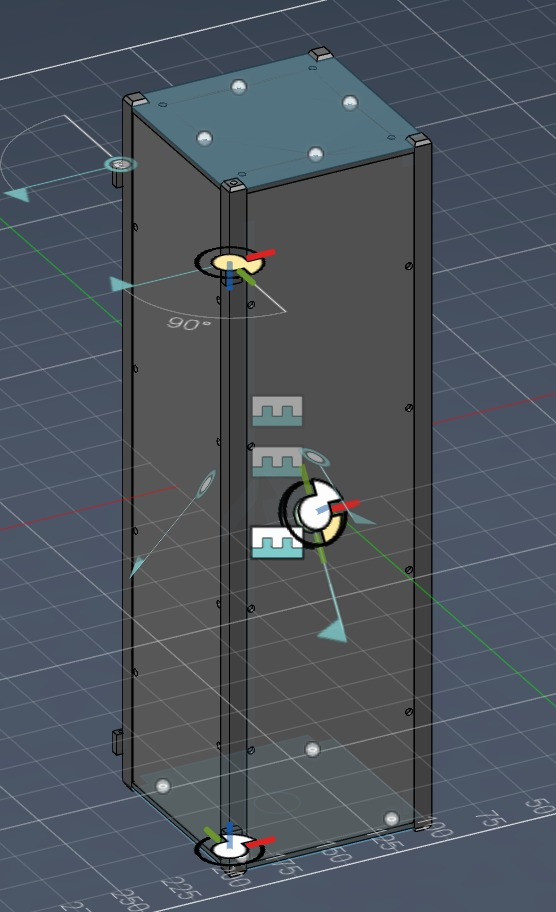
\includegraphics[width=\columnwidth]{figures/cad_chassis.jpg}
\caption{3U CubeSat chassis with shear side panels and rail structure.}
\label{fig:cad_chassis}
\end{figure}

\subsection{Reaction wheel assembly and mounting}
\label{sec:cad_rwa}

The array is three wheels in a mutually orthogonal set, each tilted
$\theta=\arccos(1/\sqrt3)\approx54.74^\circ$ from $+z$ and spaced $120^\circ$
apart in azimuth ($0^\circ,120^\circ,240^\circ$) --- the CAD counterpart of
\cref{eq:Amatrix,eq:Amatrix_num} and, unlike the earlier pyramid, an exact
match to what the simulation flies.

\begin{figure}[!t]
\centering
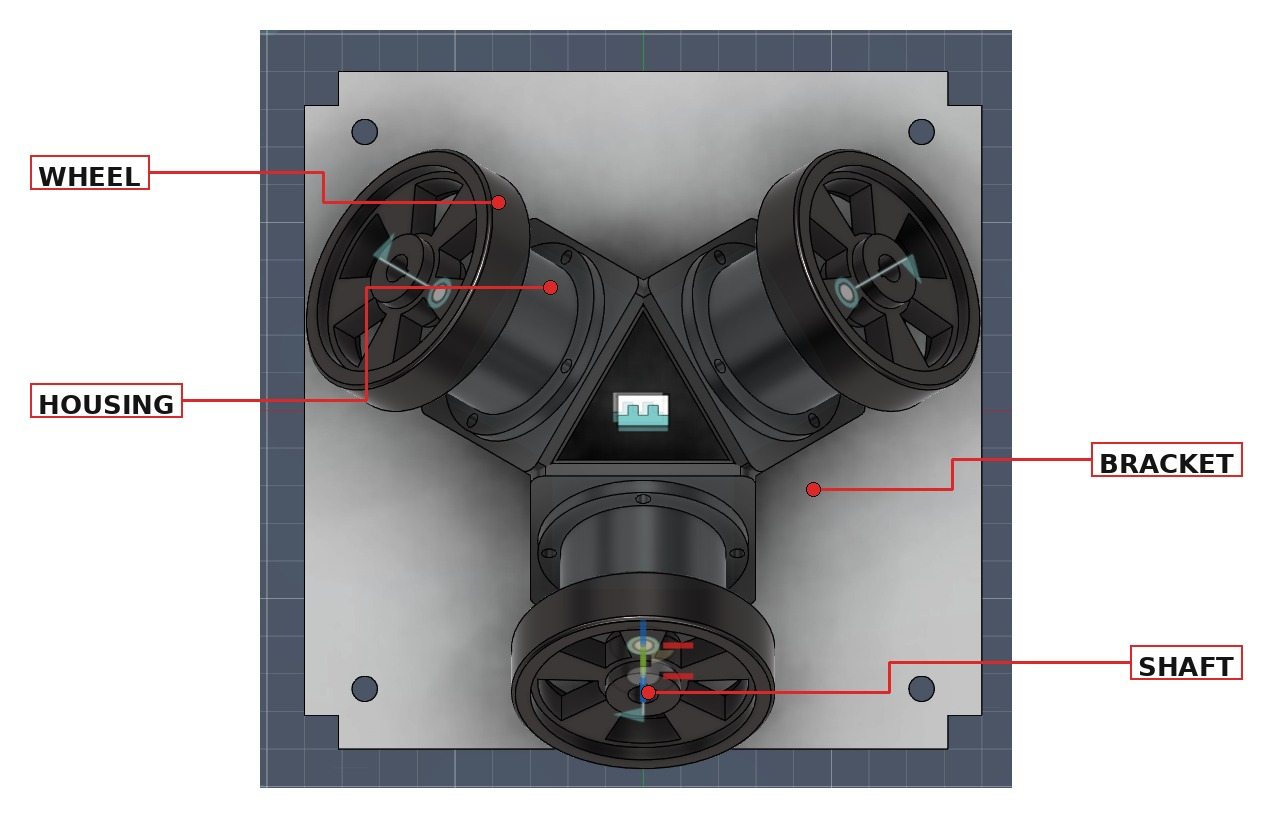
\includegraphics[width=\columnwidth]{figures/cad_rwa.jpg}
\caption{Reaction-wheel assembly, orthogonal configuration. Three wheels at
$120^\circ$ azimuth, each canted $54.74^\circ$ from $+z$, on a common bracket.}
\label{fig:cad_rwa}
\end{figure}

\begin{figure}[!t]
\centering
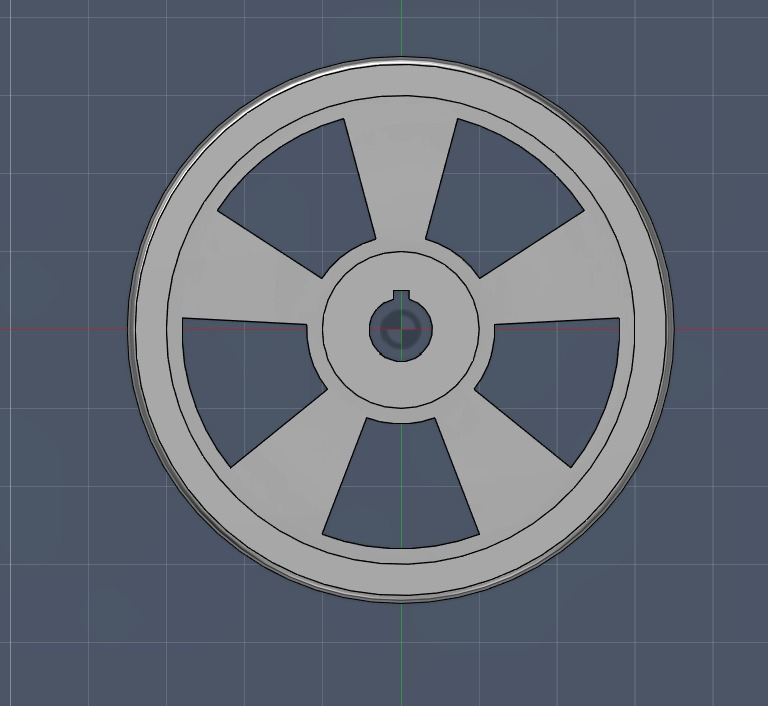
\includegraphics[width=0.72\columnwidth]{figures/cad_wheel.jpg}
\caption{Reaction-wheel rotor. The spoked web places mass at the rim, which is
what makes $I_w$ large for a given wheel mass and sets the momentum envelope of
\cref{tab:envelope}.}
\label{fig:cad_wheel}
\end{figure}

Each wheel is driven by a Maxon ECX Flat 22L brushless motor \cite{maxon},
chosen for its flat form factor (fits the assembly inside the 3U envelope
without extending the wheel bay), brushless construction (no brush wear over a
mission where the wheels run near-continuously in hold mode), fine repeatable
torque control with integrated Hall-sensor speed feedback, and low mass at
$22\unit{mm}$ diameter.

The flywheel uses a 5-spoke design rather than a solid disc: for equal total
mass, concentrating material at the rim gives more spin-axis inertia than a
solid disc, so more stored momentum per gram of flywheel. Each flywheel gives
$I_w=5.8\times10^{-6}\unit{kg\,m^2}$ at $31.116\unit{g}$, the value
\cref{tab:massprops} already carries. Each wheel mounts on an inclined bracket
whose face-normal tilt ($35.26^\circ$, the complement of $54.74^\circ$) sets
the cant; the bracket transfers reaction torque into the central bulkhead
through a bolted base flange and four motor-mount screws.

\begin{figure}[!t]
\centering
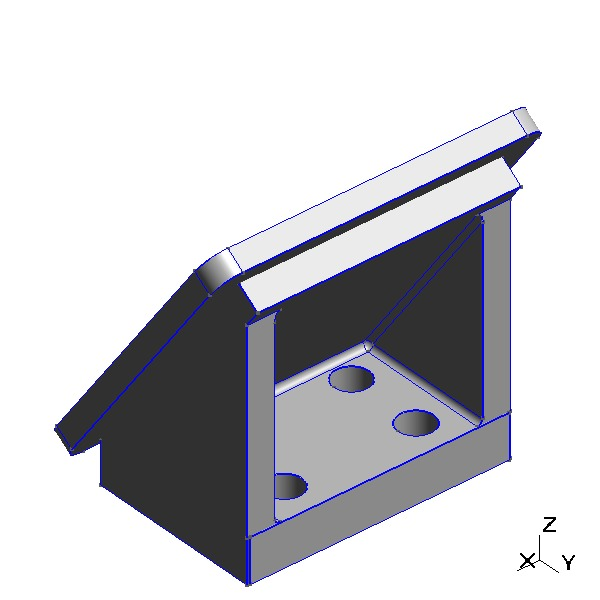
\includegraphics[width=\columnwidth]{figures/cad_bracket.jpg}
\caption{Single reaction wheel and mounting bracket.}
\label{fig:cad_bracket}
\end{figure}

\subsection{Magnetorquer hardware}
\label{sec:cad_mtq}

\Cref{sec:desat} gives the desaturation law; this subsection sizes the rods it
drives. The layout is two torque rods along body $X$/$Y$ plus one flat air-core
coil on the top bulkhead for $Z$, since a rod of useful length does not fit
along the short axis.

The X/Y rods use a ferromagnetic (steel) core with a copper winding: a
high-permeability core concentrates flux and amplifies the achievable dipole
per turn and per amp, so a core is worth the mass a plain air coil would save.
Because the rod is finite, not infinite, its effective permeability is set by
the geometry through the demagnetising factor: at aspect ratio 15
($60\times4\unit{mm}$), $N_d=0.0107$ and the effective rod permeability is
$\mu_\text{rod}\approx86$ from a relative core permeability of $\mu_r=1000$.
Copper is used for both windings for its low resistivity, which minimises
resistive loss for a given dipole. The $Z$ coil is air-core: a ferromagnetic
core has no benefit in a large flat loop and would only add mass, so that axis
relies on turns and enclosed area alone.

Sizing followed the environmental disturbance budget of \cref{tab:disturbances}
at $500\unit{km}$: gravity gradient, aerodynamic drag, solar pressure and the
spacecraft's own residual magnetic dipole (dominant, assuming a residual of
$0.01\unit{A\,m^2}$) total $\approx469\unit{nN\,m}$. Countering that with a
$2\times$ margin at the minimum field $B=25\unit{\mu T}$ requires
$\approx0.038\unit{A\,m^2}$ per axis; \cref{tab:magnetorquer} gives the design
actually built to that requirement, with margin over it on both geometries.

\begin{table*}[!t]
\centering
\caption{Magnetorquer design points. Combined worst-case power draw across all
three axes is under $120\unit{mW}$.}
\label{tab:magnetorquer}
\footnotesize
\begin{tabularx}{\textwidth}{@{}lXlccccc@{}}
\toprule
\textbf{Axis} & \textbf{Geometry} & \textbf{Winding} & \textbf{Current} &
\textbf{Resistance} & \textbf{Power} & \textbf{Dipole} & \textbf{Margin} \\
\midrule
X/Y rod & $60\times4\unit{mm}$ steel core, $14\unit{mm}$ OD copper coil,
  $50\unit{mm}$ winding & 600 turns AWG28 & $100\unit{mA}$ & $\approx2.3\,\Omega$
  & $\approx23\unit{mW}$ & $0.065\unit{A\,m^2}$ & $+70\,\%$ \\
Z coil & $64\times64\unit{mm}$ rounded-square air coil, $6\times6\unit{mm}$
  bundle & 150 turns AWG28 & $100\unit{mA}$ & $\approx7.3\,\Omega$ &
  $\approx73\unit{mW}$ & $0.0504\unit{A\,m^2}$ & $+32.6\,\%$ \\
\bottomrule
\end{tabularx}
\end{table*}

\begin{cautionbox}[The simulation currently models one dipole limit, not two]
\Cref{tab:massprops,sec:desat} carry a single, axis-uniform
$m_\text{max}=0.2\unit{A\,m^2}$, an assumption pending exactly this hardware
design. The design above gives $0.065\unit{A\,m^2}$ on X/Y and
$0.0504\unit{A\,m^2}$ on Z, both well below the placeholder and not equal to
each other. \texttt{MagnetorquerArray} currently clips to one scalar limit for
all three axes; the more accurate value to use there today is the smaller of
the two, $0.0504\unit{A\,m^2}$, since a uniform model should use the binding
axis rather than the more generous one. \TODO{Extend
\texttt{actuators/magnetorquers.py} to accept a per-axis limit (a length-3
array clips elementwise with no other change to the law) and re-run
\cref{sec:desat_result} against it; the desaturation results in this report
were produced under the $0.2\unit{A\,m^2}$ placeholder and have not yet been
re-verified against either real figure.}
\end{cautionbox}

The decay-time-constant result already stated in \cref{sec:desat},
$\vect{\tau}=-k_\text{desat}\vect{h}_{w\perp}$, describes the instantaneous
perpendicular component. Orbit-averaging as $\vect{B}$ sweeps through the body
frame ($\langle\sin^2\theta\rangle=2/3$) gives the decay of the full stored
momentum vector,
\begin{equation}
\|\vect{h}_w(t)\| \approx \|\vect{h}_w(0)\|\,e^{-t/\tau_c},
\qquad
\tau_c = \frac{3}{2k_\text{desat}},
\label{eq:mtqtau}
\end{equation}
which for the $k_\text{desat}=5\times10^{-3}\unit{s^{-1}}$ used in this project
gives $\tau_c\approx300\unit{s}$, about $5\,\%$ of one orbital period. Per orbit
the disturbance budget above delivers $\approx2.66\times10^{-3}\unit{N\,m\,s}$
of momentum to absorb; a target time constant of one fifth of an orbit
($\approx1135\unit{s}$) would set $k_\text{desat}\approx1.32\times10^{-3}
\unit{s^{-1}}$, slower than the value actually used and left as a tuning note
rather than a change, since \cref{sec:desat_result} already demonstrates
desaturation working at the faster rate.

\subsection{Materials and mass budget}
\label{sec:cad_mass}

Aluminium alloys dominate the load-bearing structure: 6061 where machinability
matters, 7075 where stress concentration is higher. The flywheel rim is
stainless steel, to maximise rim density and spin-axis inertia for a given
flywheel mass. The avionics and payload stack is modelled as FR4 PCB with
assorted components.

\begin{cautionbox}[Mass has grown with the redesign; the new total is not yet tabulated]
The three-wheel cone and the deployable solar array of \cref{sec:cad_solar}
both add mass the earlier four-wheel component budget did not carry, so that
budget (and its $1.765\unit{kg}$ total) no longer applies and is not
reproduced here. \Cref{tab:massprops}'s $m=3.9\unit{kg}$ therefore remains an
assumption, not a CAD measurement, until the mass budget is regenerated
component-by-component against the current design and \texttt{SPACECRAFT\_
MASS\_KG} is set from that export rather than the reverse.
\end{cautionbox}

\subsection{Deployable solar array and power budget}
\label{sec:cad_solar}

Power comes from a hybrid array: two deployable wings plus body-mounted cells.
Each wing is an FR4 substrate carrying triple-junction GaAs cells, stowed flat
against a side face within the CDS deployable allowance and released by a
burn-wire hold-down onto a hinge (\cref{fig:cad_solar}). The wings are
constrained by the CubeSat's own hold-down, not the dispenser walls, as the
specification requires.

\begin{figure}[!t]
\centering
\begin{subfigure}[t]{0.47\columnwidth}
\centering
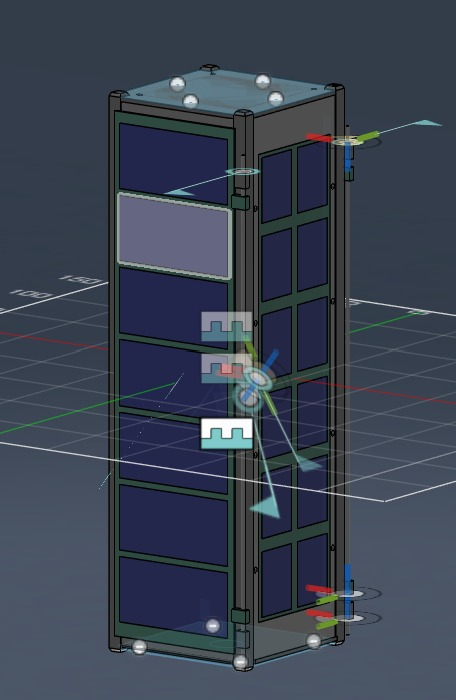
\includegraphics[width=\textwidth]{figures/cad_solar_stowed.jpg}
\caption{Stowed}
\end{subfigure}
\hfill
\begin{subfigure}[t]{0.47\columnwidth}
\centering
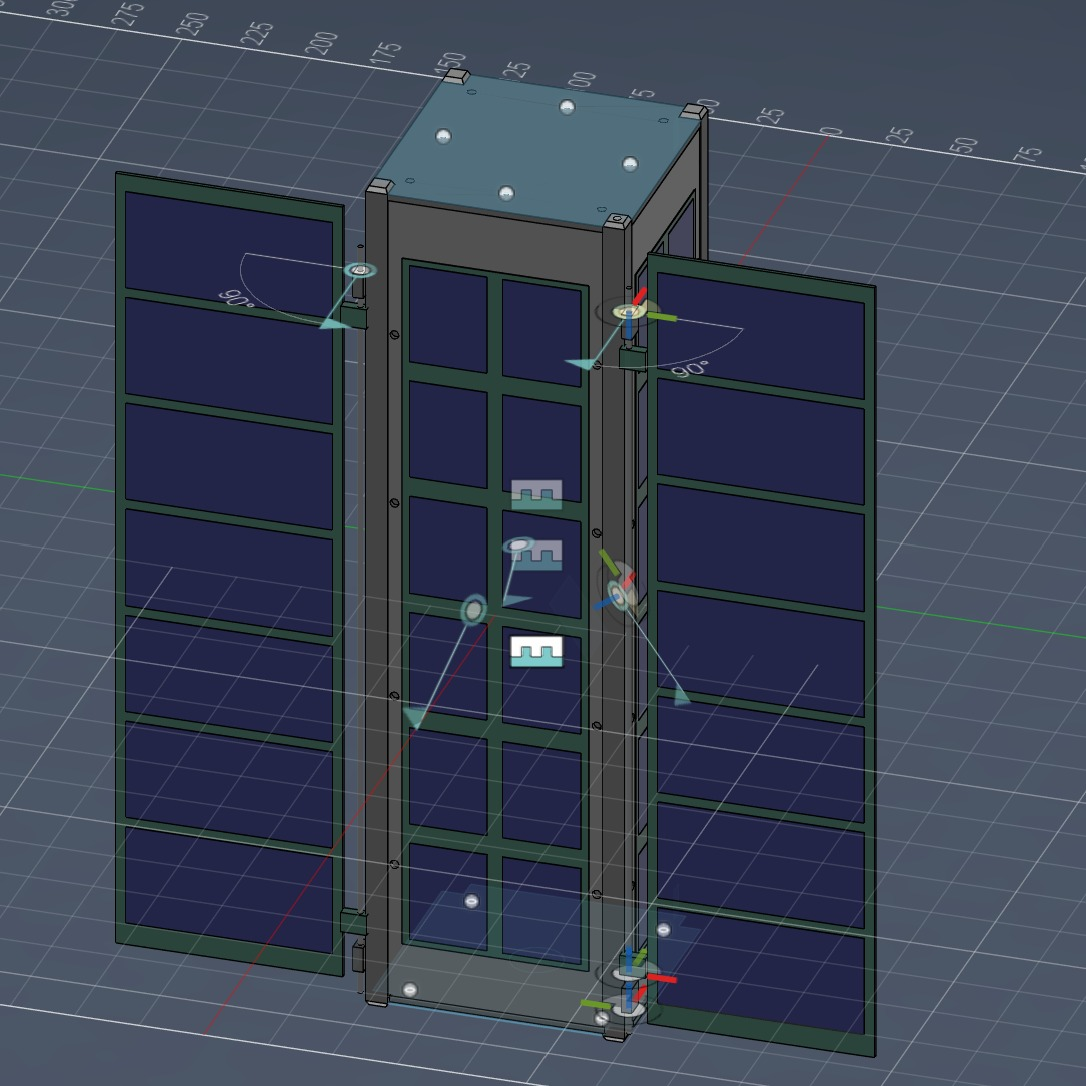
\includegraphics[width=\textwidth]{figures/cad_solar_deployed.jpg}
\caption{Deployed}
\end{subfigure}
\caption{Deployable solar wing, stowed vs.\ deployed.}
\label{fig:cad_solar}
\end{figure}

The array carries 62 triple-junction GaAs cells (28\,\% BOL efficiency)
totalling $1024\unit{cm^2}$: $448\unit{cm^2}$ across the two wings (14 cells,
$80\times40\unit{mm}$) and $576\unit{cm^2}$ body-mounted across the four side
faces (48 cells, $30\times40\unit{mm}$). The nadir face carries no cells
(payload aperture) and the zenith cap is bare (structural interfaces).
Body-mounted cells alone would average only $\approx2\unit{W}$ per orbit --- a
negative budget, and the commonest CubeSat power failure --- so the wings are
mission-critical: they roughly triple the sun-facing area.

At normal incidence the theoretical peak is $\approx39\unit{W}$
($1361\unit{W/m^2}\times1024\unit{cm^2}\times0.28$, matching
\texttt{constants.py}'s \texttt{SOLAR\_PEAK\_POWER\_W} exactly). After eclipse
($\approx38\,\%$ of each orbit) and incidence-angle losses, orbit-averaged
generation is $\approx8.5\unit{W}$, again matching the constant the simulation
uses. The estimated orbit-average load is dominated by the ADCS: operating the
wheels in a momentum-hold-dominant profile with slew transients buffered by the
battery draws $\approx2.5$--$3\unit{W}$; other subsystems and EPS losses bring
the total to $\approx4.7$--$5.2\unit{W}$, close to the itemised $4.3$--$5.6
\unit{W}$ (with margin) in \cref{tab:disturbances}'s companion power analysis.
Generation against load gives a margin of roughly $1.6$--$1.8\times$, inside
standard CubeSat practice ($1.3$--$2\times$) and with headroom for cell
degradation.

\subsection{Inertia tensor and centre of mass}
\label{sec:inertia}

The tensor was exported from Fusion 360 in $\mathrm{g\,mm^2}$ and converted.
Deploying the wings moves mass outboard, so the CAD reports both
configurations; the controller operates deployed, so the deployed tensor is
the one that matters for control design.

\begin{table*}[!t]
\centering
\caption{CAD-extracted inertia tensor about the centre of mass, stowed and
deployed. See the caution box below for how this relates to \cref{eq:inertia}.}
\label{tab:inertia}
\footnotesize
\begin{tabular}{@{}llc@{}}
\toprule
\textbf{Configuration} & \textbf{Symbol} & \textbf{Value} \\
\midrule
Stowed, about CoM & $\mat{J}_\text{stowed}$ &
$\begin{bmatrix}
3.453\times10^{-2} & -5.053\times10^{-6} & -1.662\times10^{-5}\\
-5.053\times10^{-6} & 3.421\times10^{-2} & 5.968\times10^{-5}\\
-1.662\times10^{-5} & 5.968\times10^{-5} & 8.357\times10^{-3}
\end{bmatrix}\unit{kg\,m^2}$, CoM $(-0.271,\,0.367,\,0.596)\unit{mm}$ \\[24pt]
Deployed, about CoM & $\mat{J}_\text{deployed}$ &
$\begin{bmatrix}
3.616\times10^{-2} & 5.311\times10^{-6} & -2.115\times10^{-5}\\
5.311\times10^{-6} & 3.452\times10^{-2} & 5.929\times10^{-5}\\
-2.115\times10^{-5} & 5.929\times10^{-5} & 1.030\times10^{-2}
\end{bmatrix}\unit{kg\,m^2}$, CoM $(-2.871,\,0.57,\,0.60)\unit{mm}$ \\
\bottomrule
\end{tabular}
\end{table*}

Both configurations are diagonal-dominant, off-diagonal terms below
$0.85\,\%$ of the smallest diagonal term, a principal-axis misalignment under
$0.5^\circ$ --- the body frame is effectively principal, matching what
\cref{sec:mission} already assumed. Deploying the wings raises $J_{zz}$ from
$8.36\times10^{-3}$ to $1.03\times10^{-2}\unit{kg\,m^2}$ as mass moves outboard,
and shifts the CoM $\approx2.6\unit{mm}$ in $X$ toward the wings, both
physically expected; the deployed CoM offset sets the moment arm for the
aerodynamic- and solar-pressure disturbance torques in \cref{tab:disturbances}.

\begin{cautionbox}[This tensor is close to, but not identical to, the one the control design used]
$\mat{J}_\text{deployed}$ above and the $\mat{J}$ of \cref{eq:inertia} agree to
within $1$--$3\,\%$ per diagonal axis ($3.616$ vs $3.6050$, $3.452$ vs
$3.4500$, $1.030$ vs $1.0160$, all $\times10^{-2}\unit{kg\,m^2}$) and disagree in
sign on the small $xy$ off-diagonal term. \texttt{constants.py} and every
downstream number in this report (the bandwidth bound of \cref{eq:bwbound},
the asymmetry ratios of \cref{eq:asymmetry}, the gains of \cref{sec:gains},
every closed-loop result in \cref{sec:results}) are built on
\cref{eq:inertia}'s value, not this section's. Given the size of the gap, that
is very unlikely to change any qualitative conclusion in this report, but it
has not been re-verified: \TODO{re-run the gain design and the closed-loop
scenarios against $\mat{J}_\text{deployed}$ and confirm the deltas stay small
before treating \cref{eq:inertia} as final.}
\end{cautionbox}

\subsection{Exploded view and drawings}

The assembly follows a bottom-up sequence: the frame forms the skeleton, the
payload telescope mounts through the bottom deck, the wheel assemblies are
fitted to the central mounting plate and lowered in as a pre-assembled unit,
the avionics stack sits on the middle deck, and the top deck closes the
structure.

\begin{figure*}[!t]
\centering
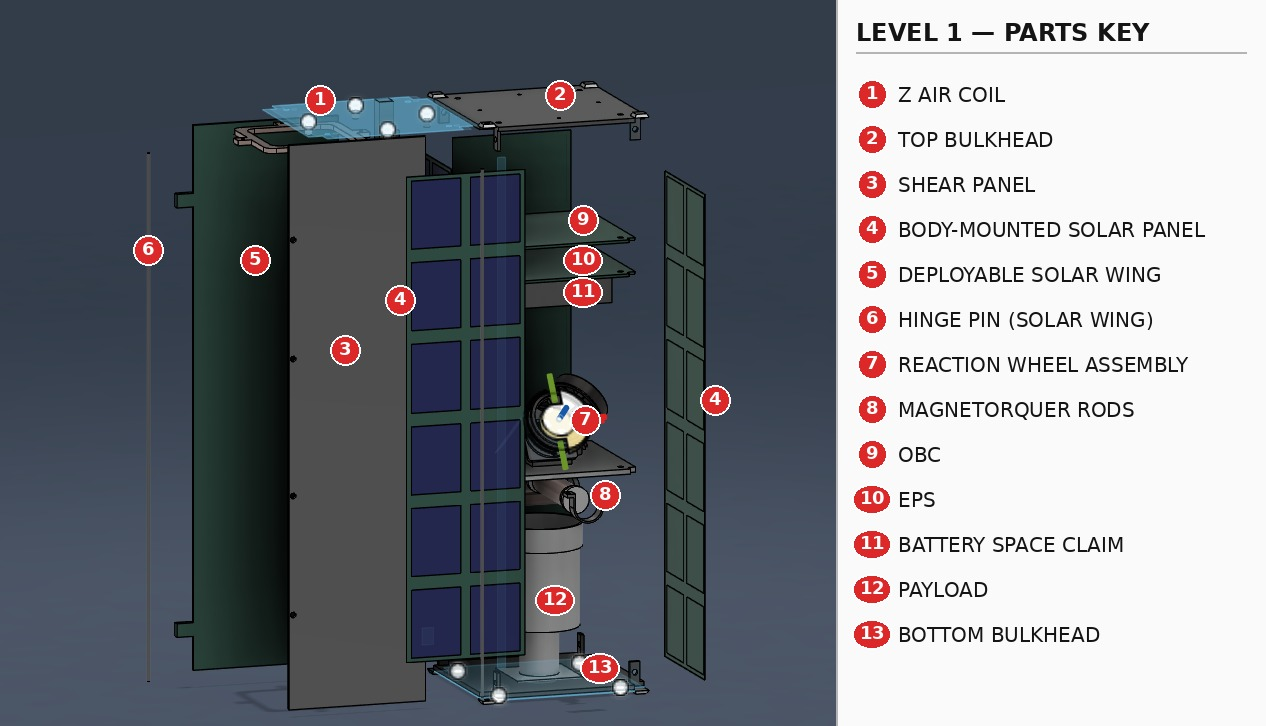
\includegraphics[width=0.85\textwidth]{figures/cad_exploded.jpg}
\caption{Labelled exploded view of the 3U assembly.}
\label{fig:cad_exploded}
\end{figure*}

\TODO{The problem statement asks for exploded views \emph{and} labelled
assembly drawings as separate mandatory items; a dimensioned drawing (principal
dimensions, rail cross-section, wheel cant and azimuth spacing) is still
needed alongside the exploded view above. Confirm the STEP and STL exports are
committed alongside the native Fusion files; the repository currently has no
\texttt{cad/} directory.}

\subsection{Structural analysis: wheel bracket FEA}
\label{sec:cad_fea}

The wheel bracket of \cref{fig:cad_bracket} holds a Maxon ECX FLAT 22 L motor
and flywheel at the wheel's $54.74^\circ$ spin-axis tilt; the motor-seating
face measured from CAD is inclined $35.26^\circ$ from the base plane, the exact
complement, confirming the bracket geometry matches the intended wheel
configuration of \cref{sec:actuators}. It was analysed under launch
quasi-static loads on the as-uploaded CAD geometry rather than a simplified
stand-in.

\paragraph{Model} Meshed in Gmsh with 24{,}332 nodes and 14{,}167 quadratic
tetrahedral elements (C3D10), refined to $0.35\unit{mm}$ near the bolt and
screw holes where stress concentration is expected; every element passed a
positive-Jacobian check before solving, ruling out inverted or degenerate
elements. The base flange and its four mounting-bolt holes were fixed,
representing a properly torqued joint. The $63.116\unit{g}$ motor-and-flywheel
assembly ($32\unit{g}$ motor, $31.116\unit{g}$ flywheel) was applied as a rigid
lumped mass coupled to the four motor-screw holes, offset $10\unit{mm}$ along
the face normal for the assembly's centre-of-gravity standoff. Each axis was
loaded separately at $12\unit{g}$ quasi-static --- the conventional
first-screening figure for a structure this size absent a launch-vehicle
spectrum, standing in for several seconds of random vibration --- with a
safety factor of $1.25$ folded into the reported margins. Al 7075-T6
($E=71.7\unit{GPa}$, $S_y=503\unit{MPa}$) is the primary material; Al 6061-T6
($S_y=276\unit{MPa}$) was checked in parallel. The two give materially the same
stress field, since stress here is governed by geometry and loading rather
than material choice, so the comparison is a secondary yield check rather than
an independent analysis.

\begin{table}[!t]
\centering
\caption{Bracket FEA results by load axis, $12\unit{g}$ quasi-static,
FoS$=1.25$. MS $=S_y/(1.25\,\sigma_\text{vM})-1$.}
\label{tab:fea}
\footnotesize
\begin{tabular}{@{}lrrrrr@{}}
\toprule
Axis & $\sigma_\text{raw}$ & $\sigma_\text{field}$ & Defl.\ & MS 7075 & MS 6061 \\
 & (MPa) & (MPa) & ($\mu$m) & & \\
\midrule
$+X$ & $2.21$ & $1.92$ & $0.19$ & $+209$ & $+114$ \\
$+Y$ & $4.15$ & $3.49$ & $0.35$ & $+114$ & $+62$ \\
$+Z$ & $4.59$ & $3.94$ & $0.34$ & $\mathbf{+101}$ & $\mathbf{+55}$ \\
\bottomrule
\end{tabular}
\end{table}

\begin{figure}[!t]
\centering
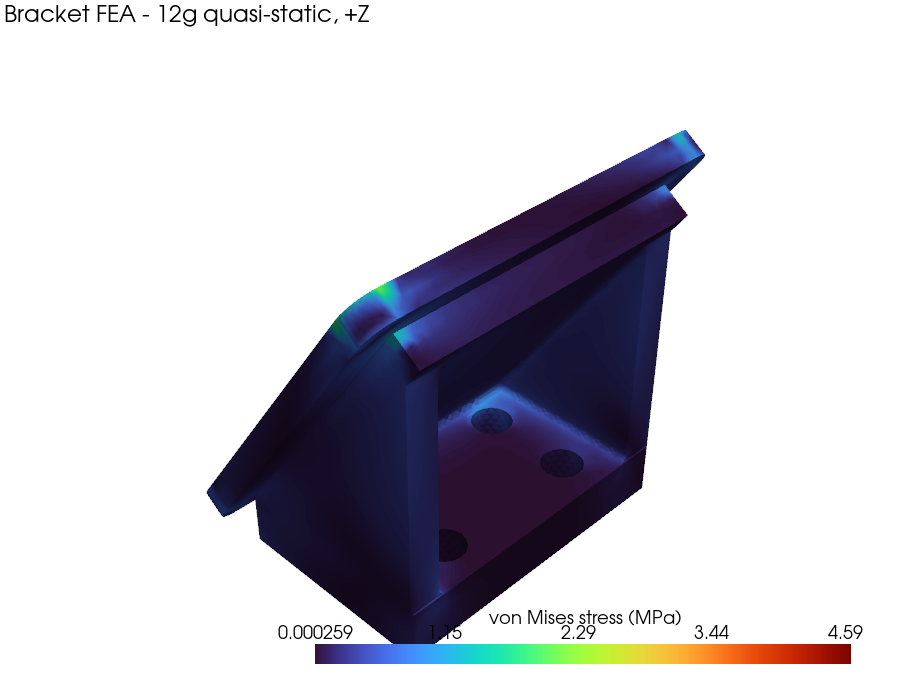
\includegraphics[width=0.85\columnwidth]{figures/fea_vonmises.png}
\caption{Von Mises stress contour, worst case ($+Z$). Peak stress sits at the
base-flange corner nearest the bolt holes, as expected for a clamped bracket
foot under load.}
\label{fig:fea_vonmises}
\end{figure}

\begin{figure}[!t]
\centering
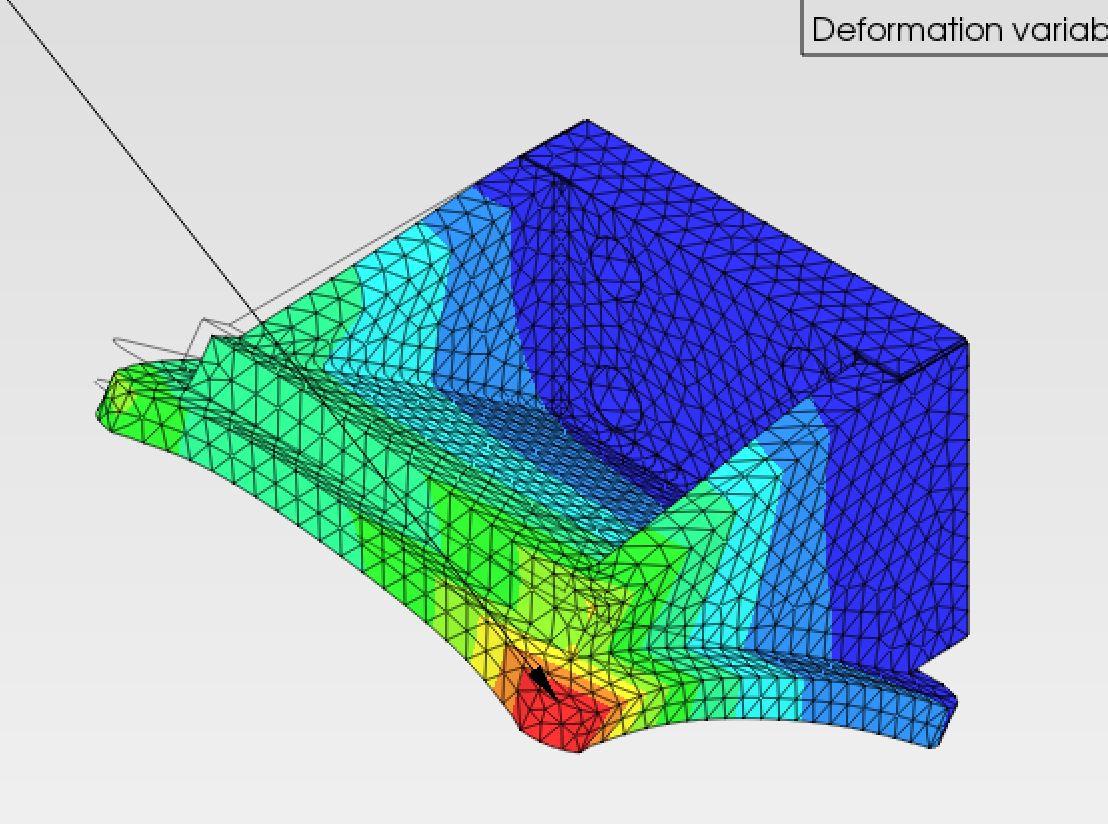
\includegraphics[width=0.85\columnwidth]{figures/fea_mesh.png}
\caption{Mesh detail at the peak-stress corner, on the deformed shape
(displacement scaled for visibility).}
\label{fig:fea_mesh}
\end{figure}

\begin{cautionbox}[The raw peak-stress column includes a boundary-singularity node]
A perfectly clamped sharp corner is a mathematical singularity: any finite
element model reports an artificially elevated, mesh-dependent stress there
that does not correspond to a physical material limit. The field column
excludes the fixed-corner/bolt-hole boundary nodes responsible for this
artefact and is the more representative figure; the conclusion --- large
margin in every case --- is unaffected either way, and \cref{tab:fea} reports
both so the reader can see the gap between them.
\end{cautionbox}

\begin{keybox}[Independently reproduced, not just computed once]
The analysis was re-run by direct execution of the CalculiX solver, separate
from the original run, on the same input deck, mesh and boundary conditions.
Peak stress and all ten natural frequencies matched exactly. Margin of safety
computed from the raw stress without excluding the boundary artefact ---
the more conservative reading, and the one that does not depend on identifying
which nodes to discard --- is $+181$, $+96$ and $+87$ for 7075-T6 across
$+X$/$+Y$/$+Z$. Even at this least favourable reading the bracket is nowhere
near its structural limit.
\end{keybox}

With stress margins of this size, stress is not the governing consideration:
the parameter that decides whether a small, stiff bracket survives launch is
its first natural frequency, since an insufficiently stiff structure risks
resonance against the launch vehicle's vibration spectrum regardless of what a
static load estimate shows. Modal analysis with the motor-and-flywheel mass
attached puts the first natural frequency at $3253\unit{Hz}$, roughly
$30\times$ above the $\sim100\unit{Hz}$ first-mode requirement typical of
CubeSat deployer specifications; the first ten modes span
$3253$--$51{,}038\unit{Hz}$. The bracket is not expected to be a resonance
risk during launch.

\begin{figure}[!t]
\centering
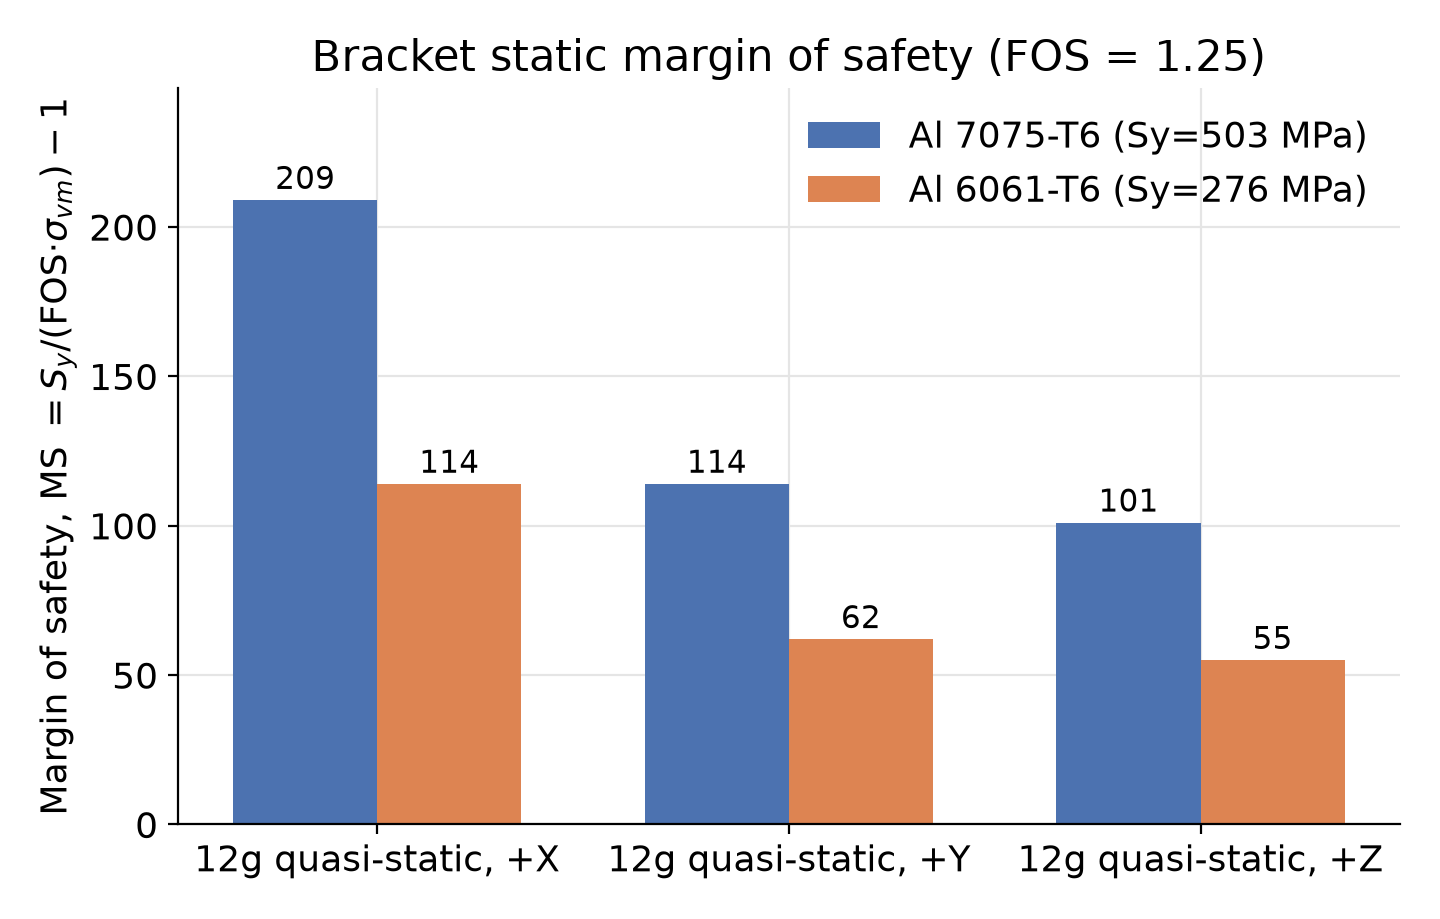
\includegraphics[width=0.95\columnwidth]{figures/fea_ms_bar.png}
\caption{Margin of safety by load direction and candidate alloy. Matches
\cref{tab:fea}'s field-stress column exactly.}
\label{fig:fea_ms_bar}
\end{figure}

\begin{figure}[!t]
\centering
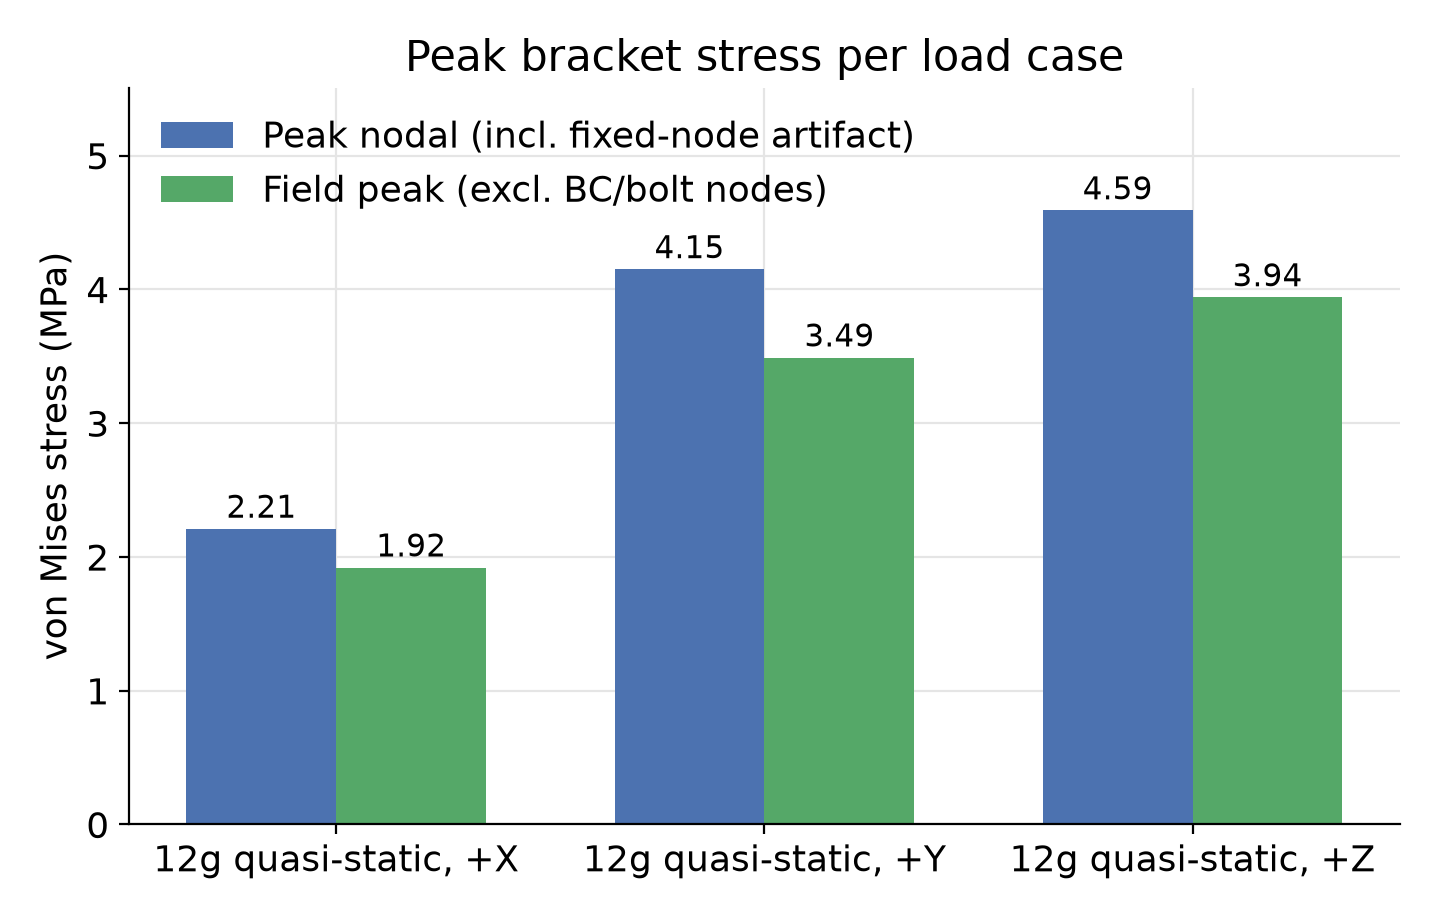
\includegraphics[width=0.95\columnwidth]{figures/fea_stress_bar.png}
\caption{Peak stress per load case: the raw (boundary-affected) value
alongside the field value that excludes it.}
\label{fig:fea_stress_bar}
\end{figure}

An earlier revision of the source write-up (\texttt{fea\_writeup\_3.pdf})
carried a version of \cref{fig:fea_ms_bar,fig:fea_stress_bar} built from a
stress dataset roughly $1.6\times$ lower than \cref{tab:fea} at every axis ---
generated, it appears, from an earlier or different solve that had not been
regenerated when the numbers in Table 1 were finalised. That has since been
corrected: the two figures above now agree with \cref{tab:fea} exactly at
every axis and alloy, and with the independently-reproduced raw-stress margins
quoted above.

This is a quasi-static equivalent on the wheel bracket alone, not a full
random-vibration PSD on the complete bus; that qualification remains future
work, alongside thermal-vacuum. Margins of this size point the other way from
a risk: the bracket is over-designed relative to the demonstrated loads, and a
future iteration has room to remove material for mass savings rather than to
add it.

%==============================================================================
\reportpart{IV}{Simulation, Verification and Results}

\section{Simulation Implementation}
\label{sec:sim}

\subsection{Architecture}

The simulation is a Python package, \texttt{deimos}, using NumPy for linear
algebra and Matplotlib for figures. Modules are small and single-purpose so
each can be tested against an analytical result in isolation.
\Cref{tab:modules} maps subpackages to what they implement, and
\cref{fig:softwarepipeline} shows how one run flows through them.

\begin{figure*}[!t]
\centering
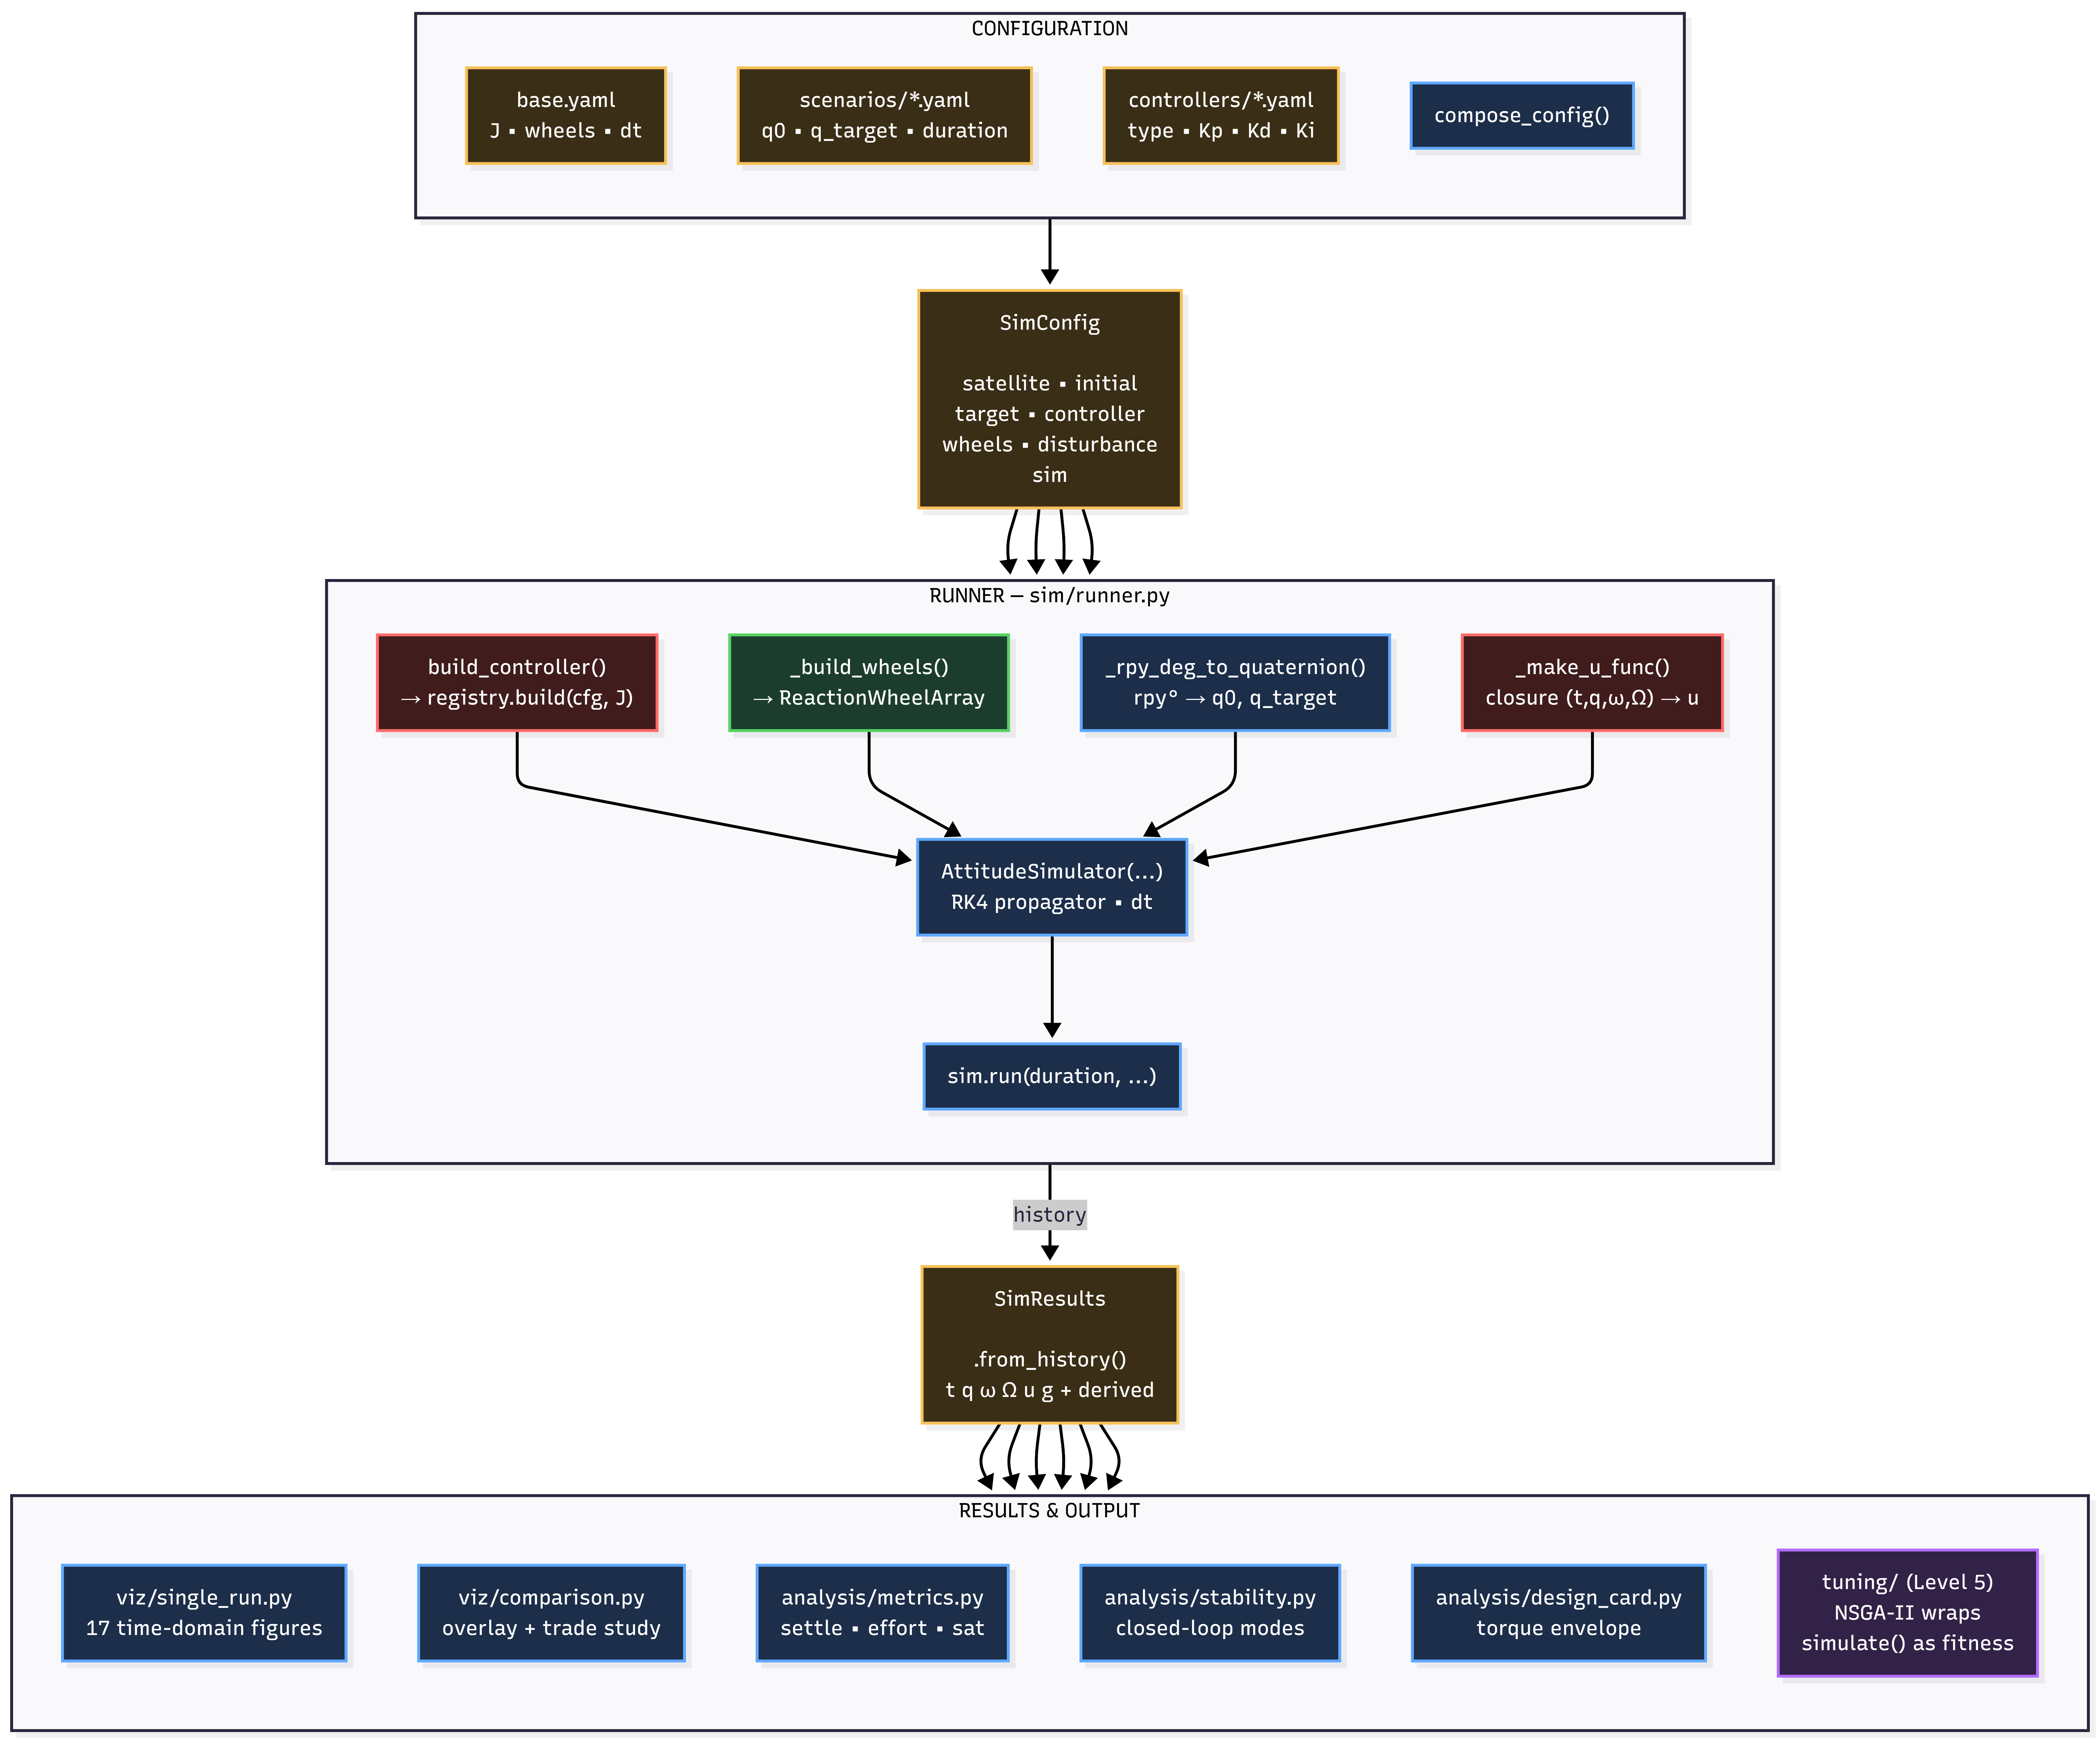
\includegraphics[width=0.86\textwidth]{figures/software_pipeline.png}
\caption{Simulation pipeline. YAML configuration is composed into a single
\texttt{SimConfig}, the runner builds the controller, wheel array and initial
state from it, and \texttt{SimResults} carries the history into every
downstream consumer. The tuning package wraps \texttt{simulate()} as a fitness
function rather than reimplementing any of it.}
\label{fig:softwarepipeline}
\end{figure*}

\begin{table*}[!t]
\centering
\caption{Package layout, \texttt{src/deimos/}.}
\label{tab:modules}
\footnotesize
\begin{tabularx}{\textwidth}{@{}p{0.20\textwidth}X@{}}
\toprule
\textbf{Subpackage} & \textbf{Contents} \\
\midrule
\texttt{constants.py} & Every parameter not being tuned: inertia tensor, wheel
and magnetorquer hardware, orbit, power budget. The single source
(\cref{sec:config}) \\[2pt]
\texttt{math/} & \texttt{quaternion.py} (algebra, error quaternion
\cref{eq:qerr}, Euler and DCM conversions), \texttt{kinematics.py}
(\cref{eq:kinematics}) \\[2pt]
\texttt{dynamics/} & \texttt{rigid\_body.py} (\cref{eq:dynamics} with the full
wheel coupling), \texttt{propagator.py} (RK4 with zero-order hold),
\texttt{disturbances.py} (\cref{eq:gg}), \texttt{environment.py} (geomagnetic
dipole field) \\[2pt]
\texttt{control/} & \texttt{wie.py} (\cref{eq:wie}, all four paper cases),
\texttt{registry.py}
(name to class), \texttt{lqr.py} (stub, see \cref{sec:future}) \\[2pt]
\texttt{actuators/} & \texttt{reaction\_wheels.py} (geometry
\cref{eq:Amatrix}, allocation \cref{eq:allocation}, sign-aware saturation),
\texttt{magnetorquers.py} (\cref{eq:mtqlaw}) \\[2pt]
\texttt{sim/} & \texttt{config.py} (YAML to typed dataclasses),
\texttt{runner.py} (the \texttt{simulate()} entry point),
\texttt{results.py} (state histories and derived metrics) \\[2pt]
\texttt{tuning/} & \texttt{nsga2.py}, \texttt{objectives.py},
\texttt{hypervolume.py}, \texttt{logbook.py}, \texttt{report.py}
(\cref{sec:ga}) \\[2pt]
\texttt{analysis/} & \texttt{metrics.py}, \texttt{stability.py} (which branch
of the Wie proof a gain set satisfies), \texttt{design\_card.py},
\texttt{power.py} \\[2pt]
\texttt{viz/} & \texttt{single\_run.py} and \texttt{comparison.py} (16 figure
types), \texttt{attitude3d.py} (3D animation), \texttt{stl\_mesh.py} (renders
the CAD mesh when an STL is supplied) \\
\bottomrule
\end{tabularx}
\end{table*}

\Cref{fig:pipeline} draws the same layout as a diagram: one
\texttt{simulate(config)} call end to end, YAML in and \texttt{SimResults} out.
It is the outer loop; \cref{fig:blockdiagram} in \cref{sec:discrete} is
everything that happens inside the \texttt{AttitudeSimulator} block here,
once per control step.

\begin{figure*}[!t]
\centering
\begin{adjustbox}{max width=\textwidth}
\begin{tikzpicture}[
  node distance=10mm and 10mm,
  pbox/.style={draw=black,rounded corners=2pt,align=center,font=\footnotesize,
               inner sep=5pt,minimum height=12mm,text width=46mm},
  wbox/.style={pbox,text width=62mm},
  gabox/.style={pbox,very thick,text width=62mm},
  sig2/.style={-{Latex[length=2mm]},draw=black,thick}]

% row 1 -- configuration
\node[pbox] (cfg) {\textbf{Configuration}\\scenario + controller YAML\\merged over \texttt{constants.py}};
\node[pbox,right=of cfg] (compose) {\textbf{compose\_config(scenario, controller)}\\deep-merge; no \texttt{\_base.yaml}};
\node[wbox,right=of compose] (simcfg) {\textbf{SimConfig}\\satellite $\cdot$ initial $\cdot$ target $\cdot$ controller\\wheels $\cdot$ magnetorquers $\cdot$ disturbance $\cdot$ sim};

% row 2 -- runner
\node[wbox,below=of cfg] (builders) {\textbf{sim/runner.py builders}\\\_build\_controller() $\to$ registry.build\\\_build\_wheels() $\to$ ReactionWheelArray\\\_build\_mtq() $\to$ MagnetorquerArray (opt.)};
\node[pbox,right=of builders] (attsim) {\textbf{AttitudeSimulator(...)}\\RK4 propagator, $\Delta t$, zero-order hold};
\node[pbox,right=of attsim] (simrun) {\textbf{sim.run(duration, ...)}};

% row 3 -- results
\node[wbox,below=of builders] (results) {\textbf{SimResults.from\_history()}\\$t,q,\omega,\Omega,u,g,m,\tau_\text{mtq}$ + derived};
\node[gabox,right=of results] (downstream) {\textbf{Downstream}\\\texttt{viz/} (17 figures + comparisons) $\cdot$\\\texttt{analysis/} (metrics, stability, design card, power) $\cdot$\\\texttt{tuning/} --- NSGA-II wraps \texttt{simulate()} as its\\fitness function (Level 5)};

\draw[sig2] (cfg) -- (compose);
\draw[sig2] (compose) -- (simcfg);
\draw[sig2] (simcfg.south) -- ++(0,-6mm) -| (builders.north);
\draw[sig2] (builders) -- (attsim);
\draw[sig2] (attsim) -- (simrun);
\draw[sig2] (simrun.south) -- ++(0,-6mm) -| (results.north);
\draw[sig2] (results) -- node[above,font=\scriptsize]{history} (downstream);

\end{tikzpicture}
\end{adjustbox}
\caption{The simulation pipeline: one \texttt{simulate(config)} call, YAML in,
\texttt{SimResults} out, figures and metrics downstream. The bold-bordered
block is the search that wraps this entire pipeline as its fitness function
(\cref{sec:ga}), not a step inside it.}
\label{fig:pipeline}
\end{figure*}

\subsection{Propagator and zero-order hold}
\label{sec:zoh}

The coupled state $\vect{x}=(\vect{q},\vect{\omega},\vect{\Omega})$ advances by
classical RK4 at fixed step $\Delta t=0.01\unit{s}$, with global error
$O(\Delta t^4)$. A fixed step was chosen deliberately: the control input is
piecewise constant, so there is a derivative discontinuity at every sample
instant, and an adaptive solver would cut its step at each one, which is wasted
work when the boundaries are known in advance.

The commanded torque is held constant across all four RK4 stages.

\begin{cautionbox}[A failure mode that looks like success]
Calling the control law from inside the derivative function is the natural way
to write the code, and it silently simulates a \emph{continuous-time}
controller. The response then looks better than the real system, and the error
grows as the sample rate falls, which is exactly where discrete effects matter
most. The propagator therefore takes the torque as an argument rather than a
callback, and allocation is evaluated once per control step.
\end{cautionbox}

Each step ends with $\vect{q}\leftarrow\vect{q}/\|\vect{q}\|$. The residual
before renormalisation is logged as a verification metric.

\subsection{Configuration}
\label{sec:config}

Every result is defined by a scenario YAML and a controller YAML, merged over a
base layer built from \texttt{constants.py}. There is no base YAML file: an
earlier \texttt{\_base.yaml} drifted out of sync with the constants module and
ended up carrying a different inertia tensor, so it was deleted and the base
layer is now derived from the constants directly. Changing the spacecraft in
one file changes every simulation, figure and report number.

\begin{lstlisting}[caption={Scenario and controller presets. The base layer
(satellite, wheels, magnetorquer hardware) comes from
\texttt{constants.py}.},captionpos=b,label={lst:yaml}]
# configs/scenarios/slew_55_65_15.yaml
initial:
  attitude_rpy_deg: [55.0, 65.0, 15.0]
  omega: [0.0, 0.0, 0.0]
target:
  attitude_rpy_deg: [0.0, 0.0, 0.0]
sim:
  duration: 60.0

# configs/controllers/wie_eigenaxis.yaml
controller:
  type: wie
  case: eigenaxis          # K = k*J, D = d*J, mu = 1
  zeta: 1.0
  settling_time_s: 20.0
  decouple_wheel_momentum: true
\end{lstlisting}

One command runs a scenario and writes a timestamped directory containing the
config actually used, the metrics as JSON, a run manifest with the git SHA, and
every figure:

\begin{lstlisting}
deimos run --scenario configs/scenarios/slew_55_65_15.yaml \
           --controller configs/controllers/wie_eigenaxis.yaml
\end{lstlisting}

%==============================================================================
\section{Model Verification}
\label{sec:verification}

A response that looks plausible is not evidence the model is right. Every check
below compares against something known independently of the simulation: a
conservation law or an analytical solution. All run as part of the automated
suite, which is 159 cases.

\subsection{Angular momentum conservation}
\label{sec:momentum}

With no external torque, total momentum resolved in the inertial frame,
$\vect{H}^{\FI} = \mat{R}(\vect{q})(\mat{J}\vect{\omega}+\vect{h}_w)$, is
constant no matter what the controller does, because the wheels only exchange
momentum internally. This is the most useful single check in the suite: it
exercises kinematics, dynamics, wheel model and integrator at once, needs no
reference solution, and catches sign errors that are otherwise hard to find.

Measured relative drift is $4.57\times10^{-15}$ over a $200\unit{s}$
torque-free run. On closed-loop slews the total momentum magnitude stays at
$7.0\times10^{-18}\unit{N\,m\,s}$, which is machine precision against a
nominally zero initial value.

\begin{keybox}[A free correctness test on the controller]
In a rest-to-rest manoeuvre from zero body rate and zero wheel momentum, total
momentum is zero throughout, so wheel momentum must return to zero as the body
rate does. Any residual wheel speed at the end of such a run is a bug rather
than a control design issue. This check is what failed persistently until the
$\vect{\omega}\times\vect{h}_w$ term was restored to \cref{eq:dynamics}.
\end{keybox}

\subsection{Energy conservation}

Torque-free and wheel-free, kinetic energy
$T=\tfrac{1}{2}\vect{\omega}\T\mat{J}\vect{\omega}$ is conserved. Measured
relative drift is $8.23\times10^{-15}$ over $200\unit{s}$. With the controller
active, energy should not be conserved; the monotone quantity is the Lyapunov
function of \cref{eq:V}.

\subsection{Quaternion norm drift}
\label{sec:normdrift}

With renormalisation disabled, $\left|\|\vect{q}\|-1\right|$ reaches
$2.22\times10^{-16}$ after $200\unit{s}$ at $\Delta t=0.01\unit{s}$, which is
round-off rather than truncation error. A sign or index error in $\mat{\Omega}$
produces a norm that drifts linearly and visibly, so this is a sharp test of
\cref{eq:kinematics}.

\subsection{Analytical motions}

Three cases with closed-form behaviour are checked: a spin about a principal
axis stays a pure spin; a torque-free axisymmetric body precesses at
$\dot\psi = J_z\omega_z/J_t$ with the transverse rate rotating in the body frame
at $\lambda=\omega_z(J_z-J_t)/J_t$; and a torque-free asymmetric body shows the
expected intermediate-axis instability with a bounded polhode.

Each is checked numerically against its closed-form solution in the automated
test suite (\texttt{tests/}); the residuals are in \cref{tab:verification}.

\begin{table*}[!t]
\centering
\caption{Verification results. All values measured from the committed code.}
\label{tab:verification}
\footnotesize
\begin{tabularx}{\textwidth}{@{}p{0.24\textwidth}Xll@{}}
\toprule
\textbf{Check} & \textbf{Expected} & \textbf{Measured} & \textbf{Verdict} \\
\midrule
Momentum conservation, torque-free & bounded near machine precision & $4.57\times10^{-15}$ rel. & pass \\
Momentum conservation, closed loop & zero throughout a rest-to-rest slew & $1.7\times10^{-17}\unit{N\,m\,s}$ & pass \\
Energy conservation, torque-free   & bounded near machine precision & $8.23\times10^{-15}$ rel. & pass \\
Quaternion norm drift              & round-off level                & $2.22\times10^{-16}$ & pass \\
Principal-axis spin                & pure spin retained             & within tolerance & pass \\
Torque-free precession             & matches analytical solution    & within tolerance & pass \\
Wheel-array orthogonality          & $\mat{A}\T\mat{A}=\mat{I}$     & $<10^{-6}$ & pass \\
Automated suite                    & all cases pass                 & 159 / 159 & pass \\
\bottomrule
\end{tabularx}
\end{table*}

\begin{cautionbox}[Two verification items are not done]
An earlier draft of this report described an independent Simulink
cross-implementation and a PySide6 tuning dashboard as completed work. Neither
exists in the repository, so both claims have been removed rather than left
awaiting numbers. The Simulink cross-check is the more valuable of the two,
because it is the only proposed check that does not share code with the Python
implementation, and it is listed in \cref{sec:future}. \TODO{If either artefact
exists outside the repository, commit it and restore the section; do not
restore the text without the artefact.}
\end{cautionbox}

%==============================================================================
\section{Simulation Results}
\label{sec:results}

Every run below uses the flown gains of \cref{tab:gains} at
$\Delta t=0.01\unit{s}$ and reproduces from a named file in
\texttt{configs/}. Two scenarios are the mission deliverable --- a large-angle
slew and a disturbance hold --- and a Monte-Carlo campaign then checks that the
result generalises beyond those two hand-picked cases. All numbers are read
straight from \texttt{SimResults}.

\subsection{Scenario A: large-angle slew}
\label{sec:scenarioA}

\textit{Scenario:} \texttt{slew\_160\_40\_30}, a $151.7^\circ$ rest-to-rest
slew to the target attitude under the \texttt{wie\_eigenaxis} preset (no
integral action). This is the sizing case for R1, R2, R3 and R7.

\begin{table}[!t]
\centering
\caption{Scenario A --- $151.7^\circ$ slew, measured.}
\label{tab:results_slew}
\footnotesize
\begin{tabular}{@{}llrr@{}}
\toprule
\textbf{ID} & \textbf{Metric} & \textbf{Target} & \textbf{Measured} \\
\midrule
R2 & Settling time to $1^\circ$ (s)  & $\le40$    & $28.91$ \\
R3 & Overshoot (deg)                 & $\le1.0$   & $0.000$ \\
R4 & Final attitude error (deg)      & $\le0.5$   & $0.0005$ \\
R5 & Residual body rate (deg/s)      & $\le10^{-3}$ & $1.4\times10^{-4}$ \\
R7 & Peak wheel torque (mN\,m)       & $\le4.0$   & $4.00$ \\
R7 & Peak wheel speed (rpm)          & $\le12{,}000$ & $10{,}398$ \\
-- & Torque-saturated timesteps (\%) & --         & $0.02$ \\
-- & Mean eigenaxis deviation (deg)  & --         & $0.00$ \\
-- & Control effort (mN\,m\,s)       & --         & $14.95$ \\
\bottomrule
\end{tabular}
\end{table}

\begin{figure*}[!t]
\centering
\begin{subfigure}{0.48\textwidth}
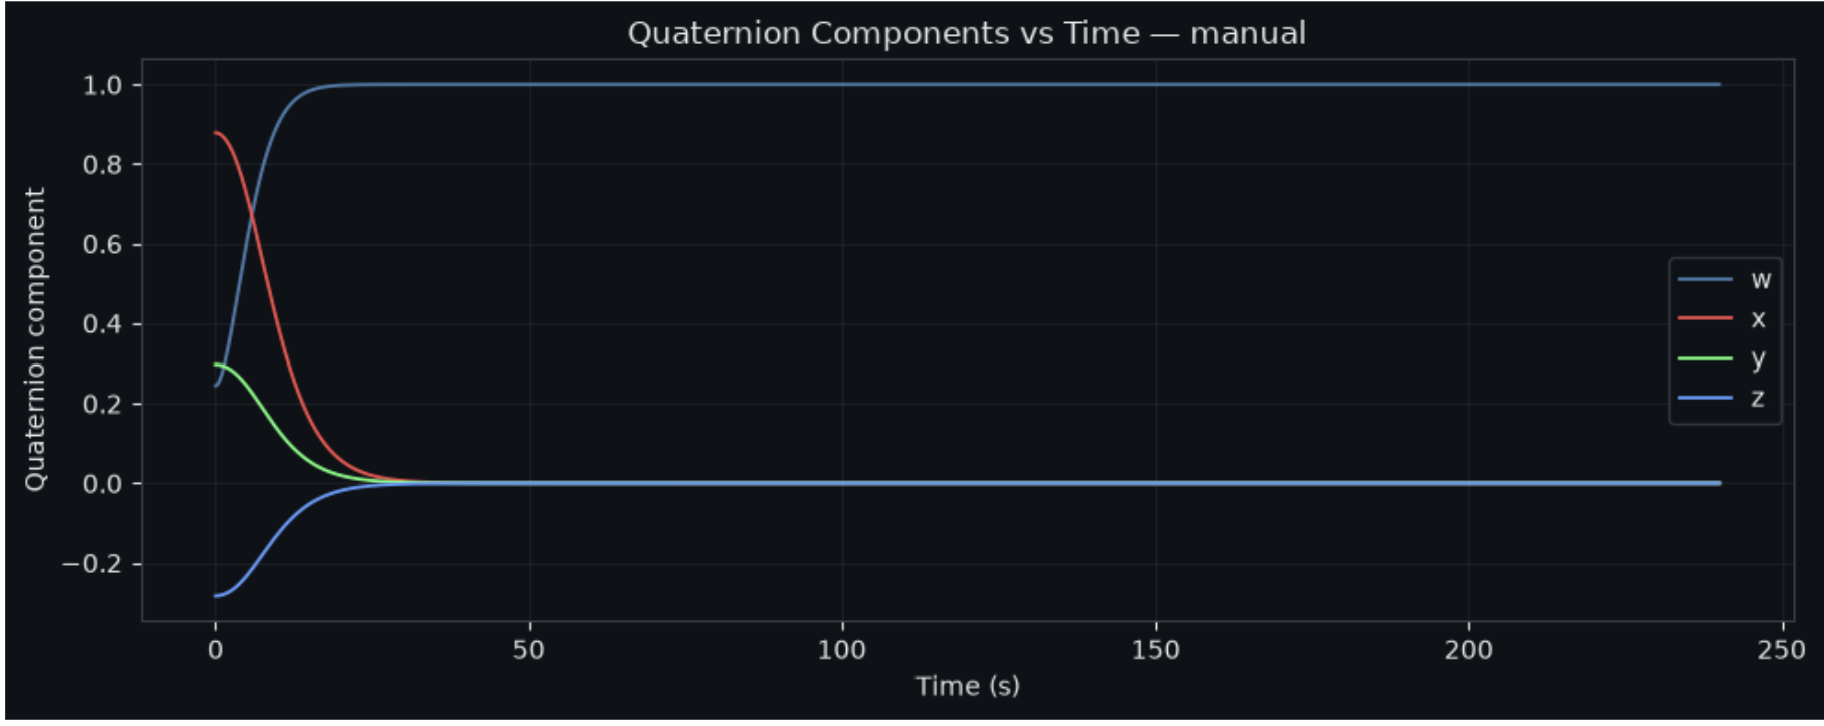
\includegraphics[width=\linewidth]{figures/simA_attitude.png}
\caption{Attitude (quaternion components).}
\end{subfigure}\hfill
\begin{subfigure}{0.48\textwidth}
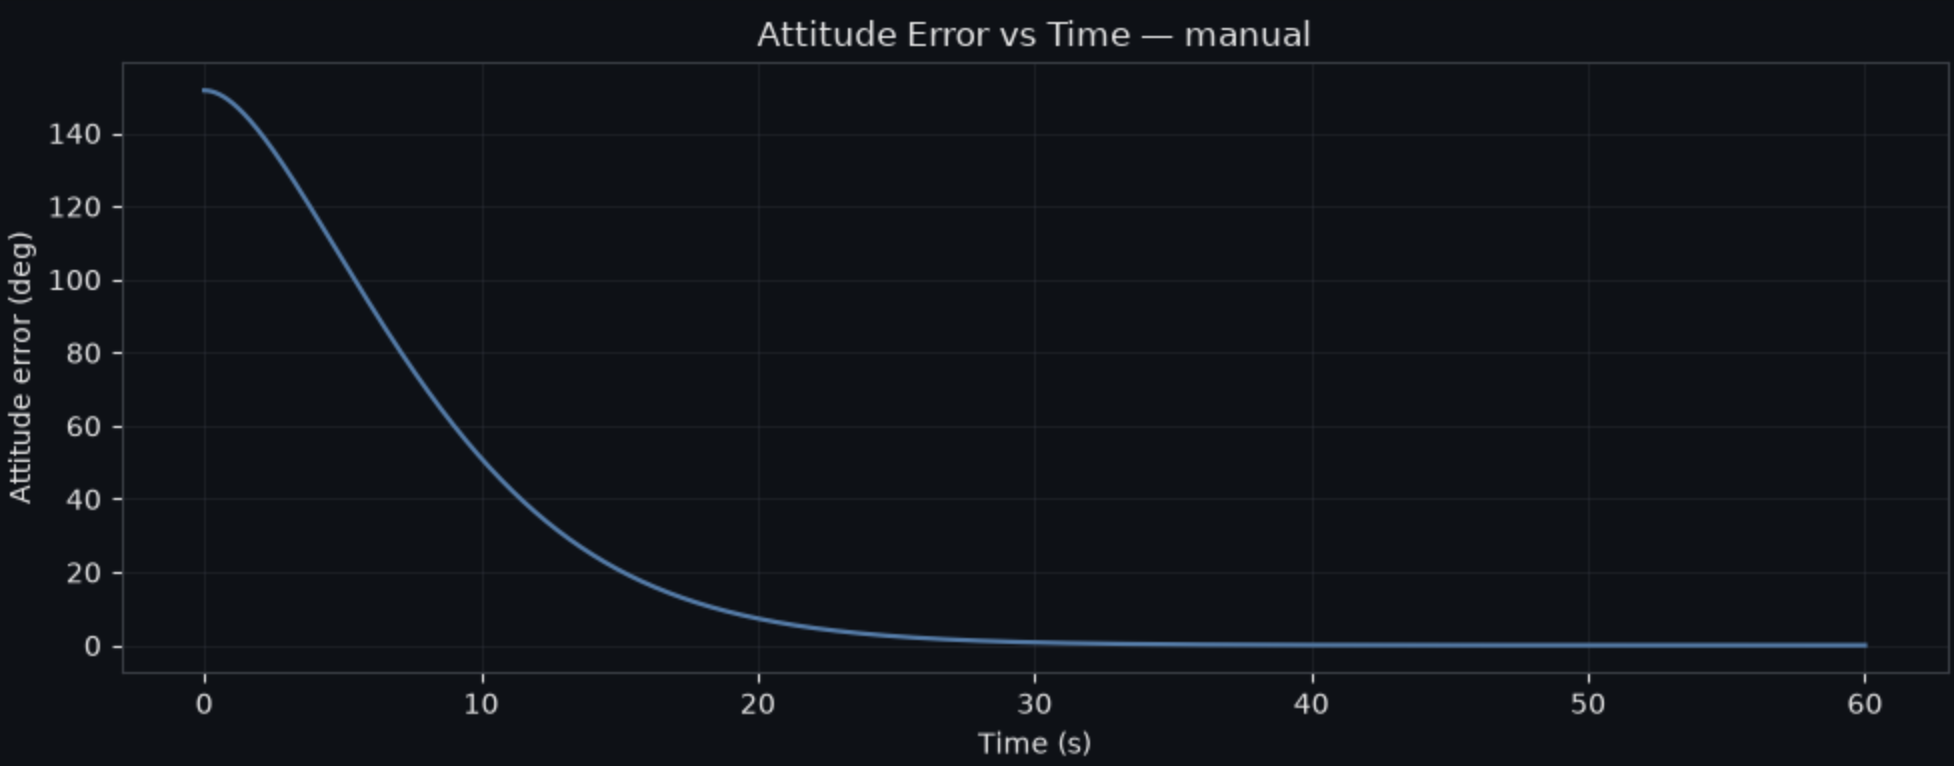
\includegraphics[width=\linewidth]{figures/simA_error.png}
\caption{Attitude error angle.}
\end{subfigure}

\vspace{4pt}
\begin{subfigure}{0.48\textwidth}
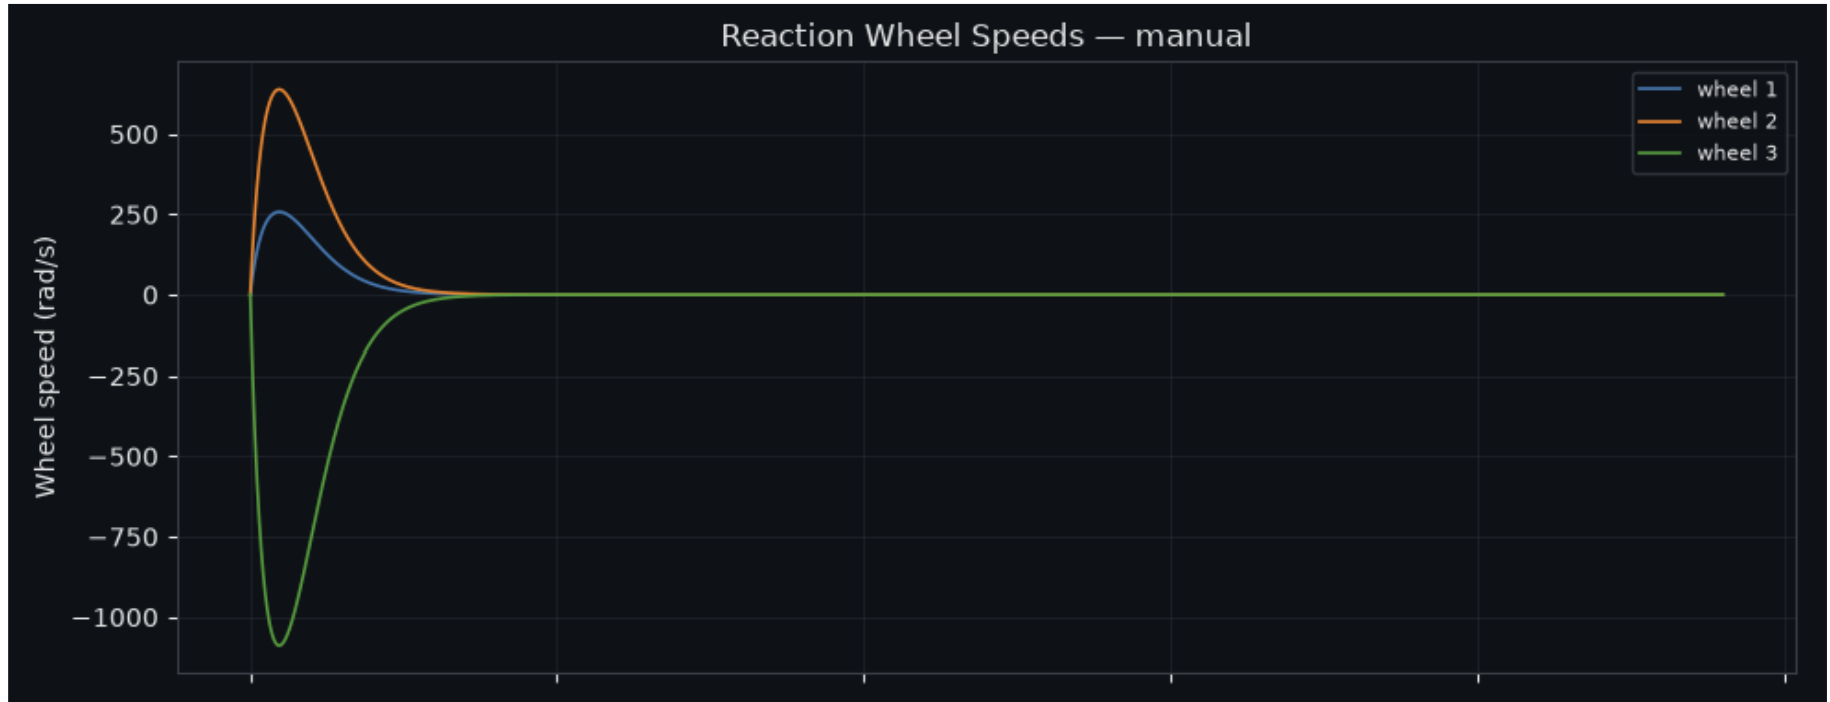
\includegraphics[width=\linewidth]{figures/simA_wheelspeed.png}
\caption{Reaction-wheel speeds.}
\end{subfigure}\hfill
\begin{subfigure}{0.48\textwidth}
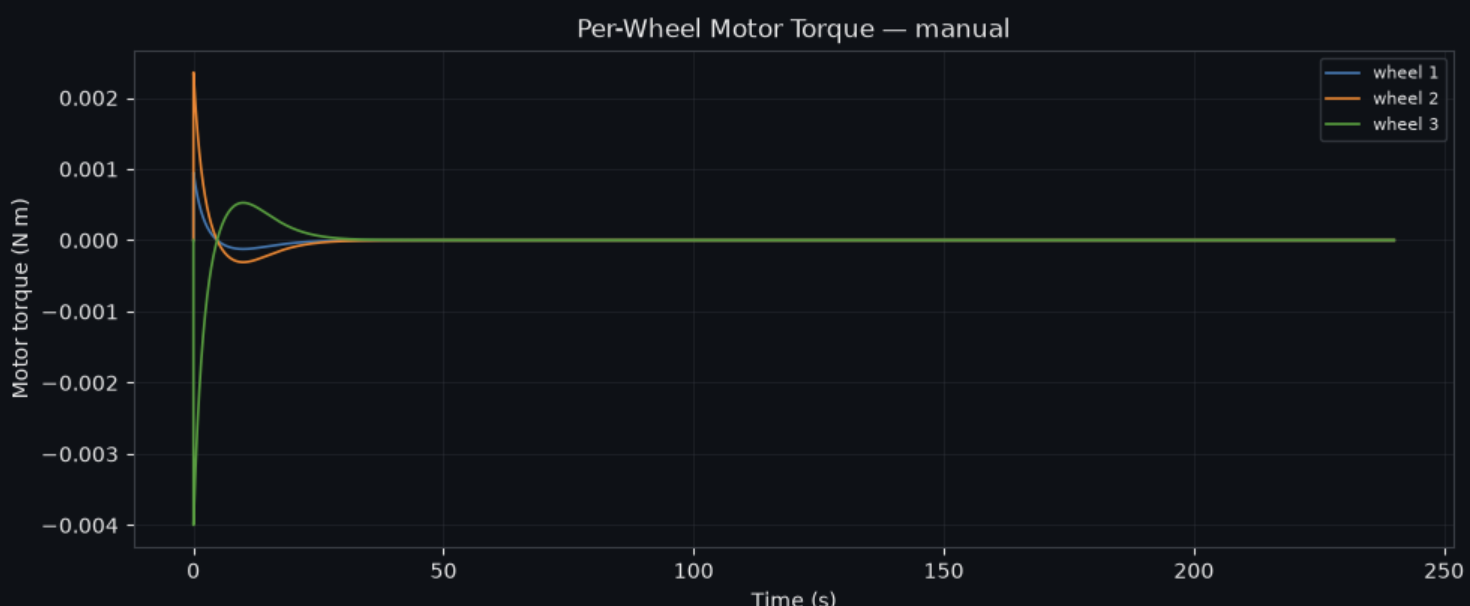
\includegraphics[width=\linewidth]{figures/simA_motortorque.png}
\caption{Per-wheel motor torque.}
\end{subfigure}
\caption{Scenario A, the four required time histories for the $151.7^\circ$
slew. The error decays monotonically to zero with no overshoot; the wheels
spin up, plateau and return to rest; the torque trace shows the single
$4\unit{mN\,m}$ clip at $t=0$ and nothing after.}
\label{fig:scenarioA}
\end{figure*}

Three things follow from \cref{tab:results_slew,fig:scenarioA}.

\emph{The slew is clean and eigenaxis-true.} The $151.7^\circ$ error decays
monotonically to $0.0005^\circ$ in $28.9\unit{s}$ with zero overshoot, and the
mean eigenaxis deviation is $0.00^\circ$ --- the spacecraft turns about the one
fixed axis the control law was chosen to deliver. Settling at $28.9\unit{s}$
is exactly what the $t_s=30\unit{s}$ sizing predicts for a slew this large; a
smaller slew settles faster (\cref{sec:validation}).

\emph{It stays inside the actuator envelope.} Peak wheel torque reaches the
$4\unit{mN\,m}$ limit for a single instant at $t=0$ --- $0.02\,\%$ of the run
--- and is unsaturated everywhere else. Peak wheel speed is $10{,}398\unit{rpm}$,
inside the $12{,}000\unit{rpm}$ limit. This is the design trade made explicit:
sizing for $30\unit{s}$ rather than $20\unit{s}$ keeps even the largest slew
essentially unsaturated, which is what lets the eigenaxis property survive
(a stiffer design clips the opening transient and loses it).

\emph{The wheels return to rest.} \Cref{fig:scenarioA}(c) shows every wheel
speed rising, plateauing and coming back to zero. That is conservation of
angular momentum, not a control choice: the body borrows momentum from the
wheels to turn and gives it back to stop, so a rest-to-rest slew is
momentum-neutral. \Cref{sec:scenarioB} is the case where it is not.

\subsection{Scenario B: hold under constant disturbance}
\label{sec:scenarioB}

\textit{Scenario:} \texttt{hold\_under\_disturbance}, an $8.5^\circ$ initial
error recovered and then held against a constant $3\times10^{-7}\unit{N\,m}$
per-axis body torque for $240\unit{s}$, under the \texttt{wie\_eigenaxis\_hold}
preset (integral action on). This exercises R4, R5 and R6.

\begin{table}[!t]
\centering
\caption{Scenario B --- disturbance hold, measured.}
\label{tab:results_hold}
\footnotesize
\begin{tabular}{@{}llrr@{}}
\toprule
\textbf{ID} & \textbf{Metric} & \textbf{Target} & \textbf{Measured} \\
\midrule
R2 & Recovery time to $1^\circ$ (s)  & $\le40$    & $13.74$ \\
R3 & Overshoot (deg)                 & $\le1.0$   & $0.021$ \\
R4 & Steady-state error (deg)        & $\le0.5$   & $0.034$ \\
R5 & Residual body rate (deg/s)      & $\le10^{-3}$ & $2.7\times10^{-5}$ \\
R7 & Peak wheel torque (\% limit)    & --         & $5.4$ \\
-- & Peak wheel speed (rpm)          & --         & $495$ \\
-- & Control effort (mN\,m\,s)       & --         & $0.88$ \\
\bottomrule
\end{tabular}
\end{table}

\begin{figure*}[!t]
\centering
\begin{subfigure}{0.48\textwidth}
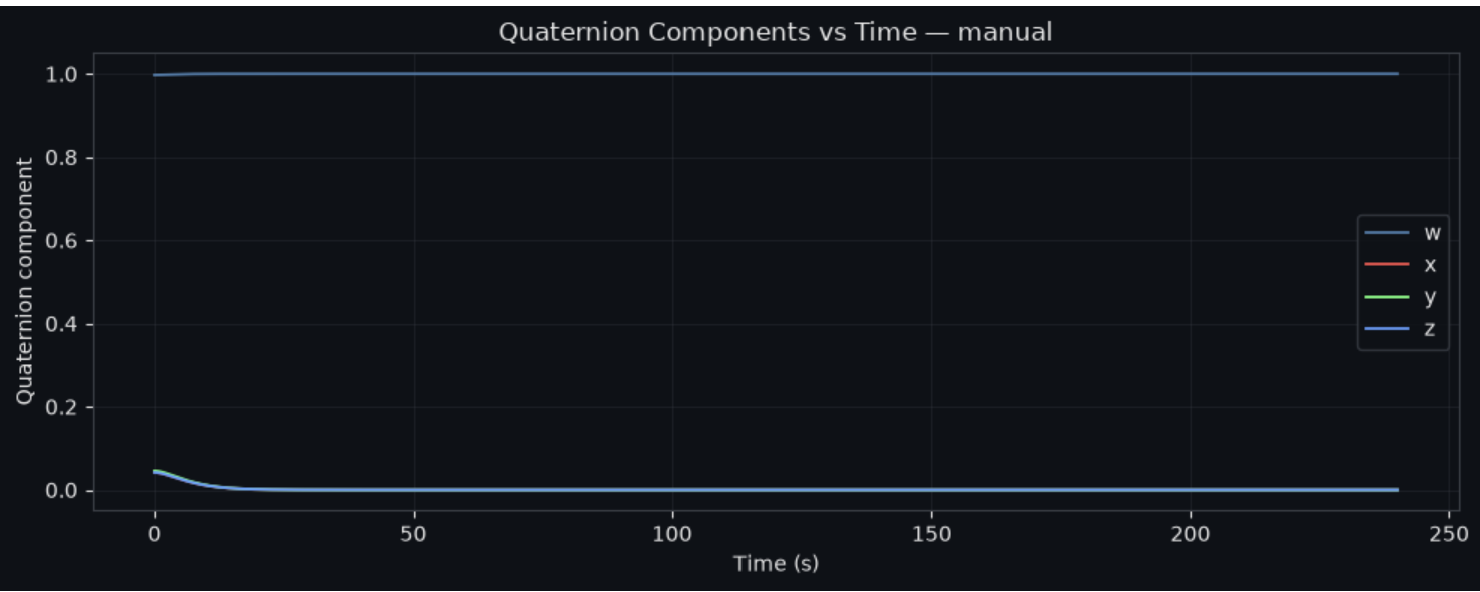
\includegraphics[width=\linewidth]{figures/simB_attitude.png}
\caption{Attitude (quaternion components).}
\end{subfigure}\hfill
\begin{subfigure}{0.48\textwidth}
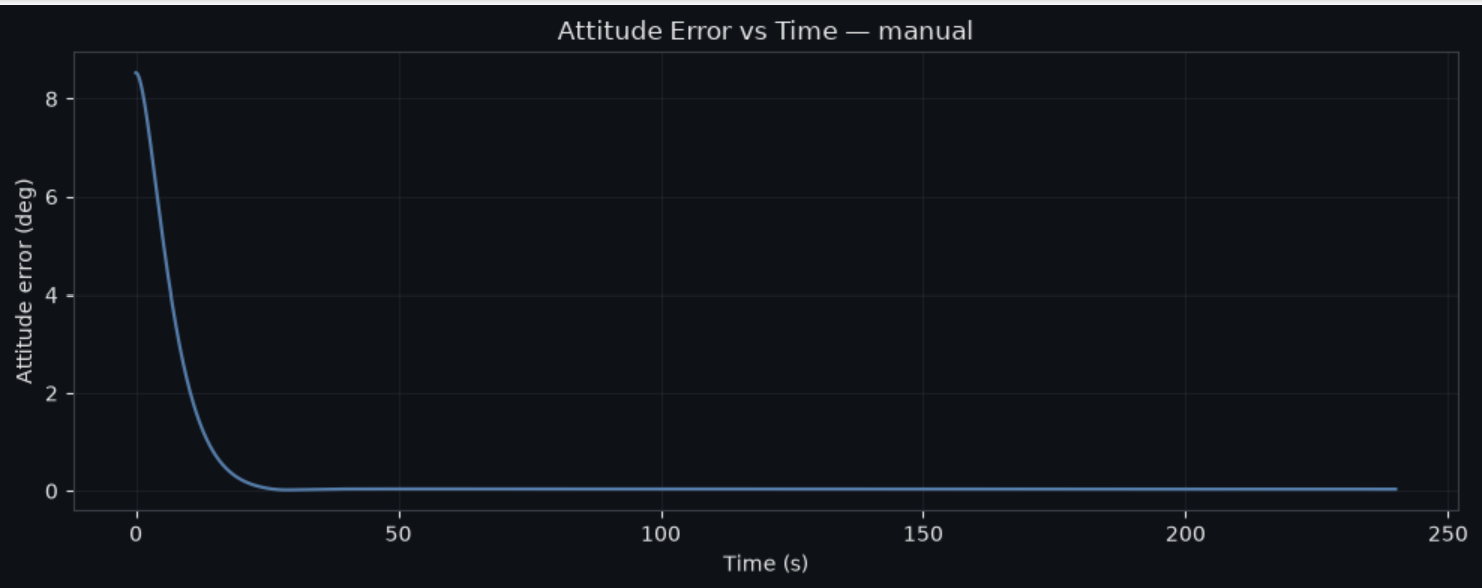
\includegraphics[width=\linewidth]{figures/simB_error.png}
\caption{Attitude error angle.}
\end{subfigure}

\vspace{4pt}
\begin{subfigure}{0.48\textwidth}
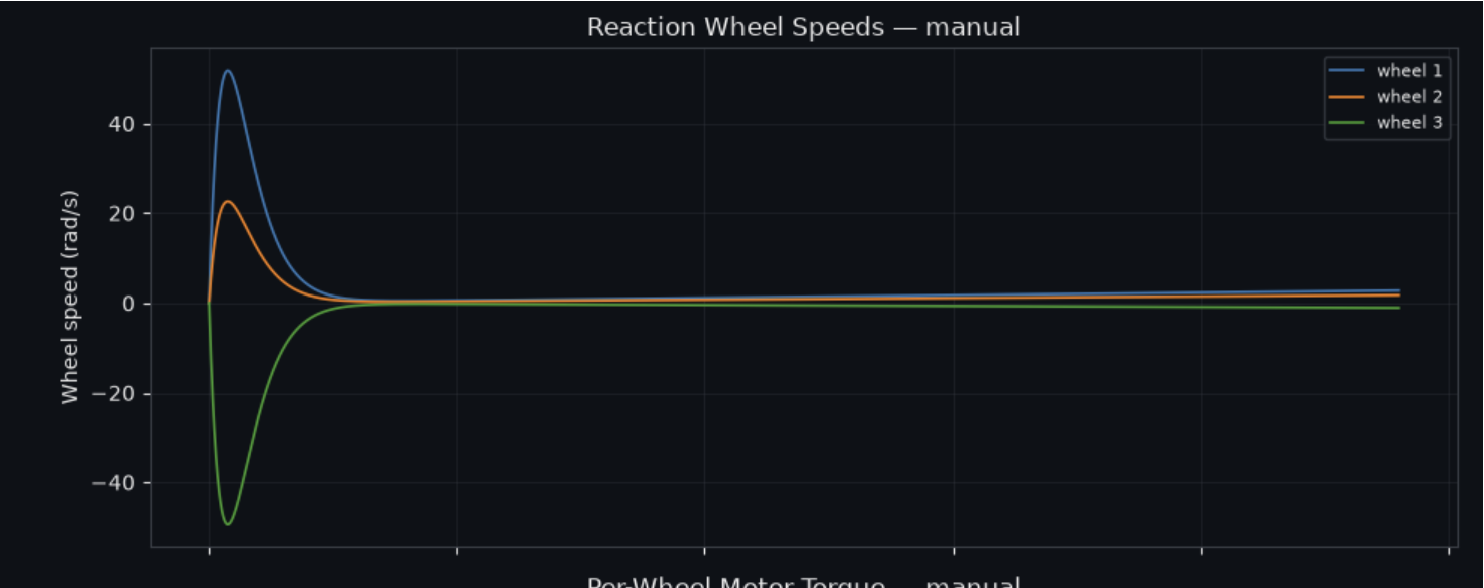
\includegraphics[width=\linewidth]{figures/simB_wheelspeed.png}
\caption{Reaction-wheel speeds.}
\end{subfigure}\hfill
\begin{subfigure}{0.48\textwidth}
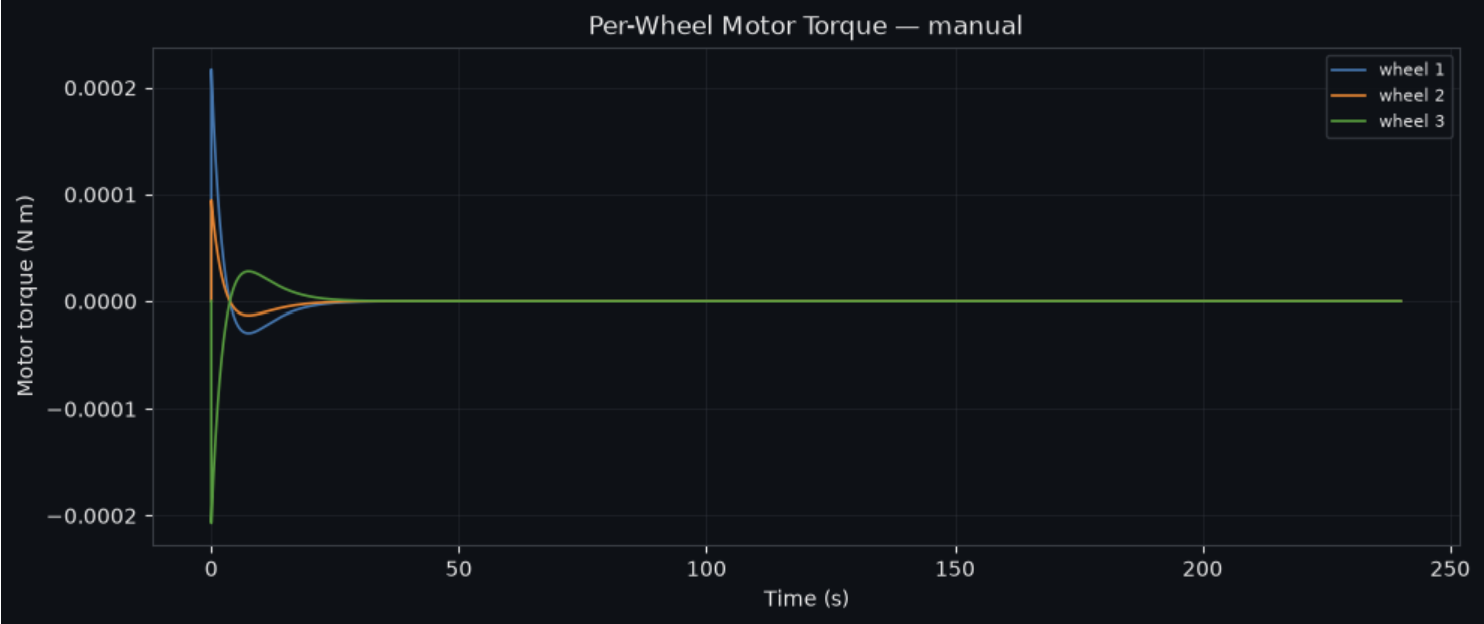
\includegraphics[width=\linewidth]{figures/simB_motortorque.png}
\caption{Per-wheel motor torque.}
\end{subfigure}
\caption{Scenario B, disturbance hold. The error is driven from $8.5^\circ$ to
below $0.05^\circ$ and held flat for the rest of the run. Note the wheel
speeds: after the initial recovery transient they do \emph{not} return to zero
but drift slowly, absorbing the constant disturbance impulse.}
\label{fig:scenarioB}
\end{figure*}

The error is recovered in $13.7\unit{s}$ and held at $0.034^\circ$ steady state
--- inside the $0.5^\circ$ requirement with an order of magnitude to spare ---
against a bias set five orders of magnitude above the true gravity gradient.
The residual body rate is $2.7\times10^{-5}\unit{deg/s}$, and peak wheel torque
never exceeds $5.4\,\%$ of the limit: holding a steady bias is a low-authority
task.

\begin{keybox}[A slew is momentum-neutral, a disturbance hold is not]
The one qualitative difference between \cref{fig:scenarioA}(c) and
\cref{fig:scenarioB}(c) is the physical heart of both scenarios. In the slew
the wheels return exactly to rest --- momentum borrowed and returned. Under a
constant disturbance they cannot: every second the bias delivers a fixed
angular impulse that the wheels must absorb, so their speed ramps secularly
and would eventually saturate. That secular ramp is precisely what the
magnetorquer desaturation of \cref{sec:desat_result} exists to bleed off, and
it is why this spacecraft needs an external momentum sink at all.
\end{keybox}

\subsection{Validation: Monte-Carlo campaign}
\label{sec:validation}
\label{sec:montecarlo}

Two scenarios cannot show that a controller works in general. The
\texttt{monte\_carlo\_verify.py} campaign samples random rest-to-rest slews ---
a uniform random rotation axis (unbiased on the sphere, not clustered the way
independent roll/pitch/yaw sampling would be) and a random angle --- and scores
each under the flown gains, with every trial reproducible from its run index.
Two regimes are run: large slews ($90$--$179^\circ$) for the manoeuvre case,
and small slews ($0$--$8^\circ$) for the fine-pointing case. The large-slew set
is also run under a tuned PID as a baseline, so the eigenaxis regulator's
numbers have something to be measured against.

\begin{table}[!t]
\centering
\caption{Monte-Carlo over 500 random $90$--$179^\circ$ slews, uniform random
axis. Mean $\pm$ standard deviation. The Wie regulator is the flown design; the
PID is a settling-time-tuned baseline.}
\label{tab:montecarlo}
\footnotesize
\begin{tabular}{@{}lrr@{}}
\toprule
\textbf{Metric} & \textbf{Wie ($k\mat{J}$)} & \textbf{PID (baseline)} \\
\midrule
Settled within cap (\%)        & $100$            & $100$ \\
Settling time (s)              & $19.0\pm1.4$     & $37.0\pm2.8$ \\
Control effort (mN\,m\,s)      & $19.4\pm6.4$     & $377.8\pm102.1$ \\
Steady-state error (deg)       & $0.097\pm0.007$  & $0.470\pm0.046$ \\
Torque saturation (\% steps)   & $2.8\pm1.5$      & $26.0\pm6.4$ \\
Mean eigenaxis dev.\ (deg)     & $6.6\pm8.0$      & $51.1\pm8.4$ \\
\bottomrule
\end{tabular}
\end{table}

\begin{figure}[!t]
\centering
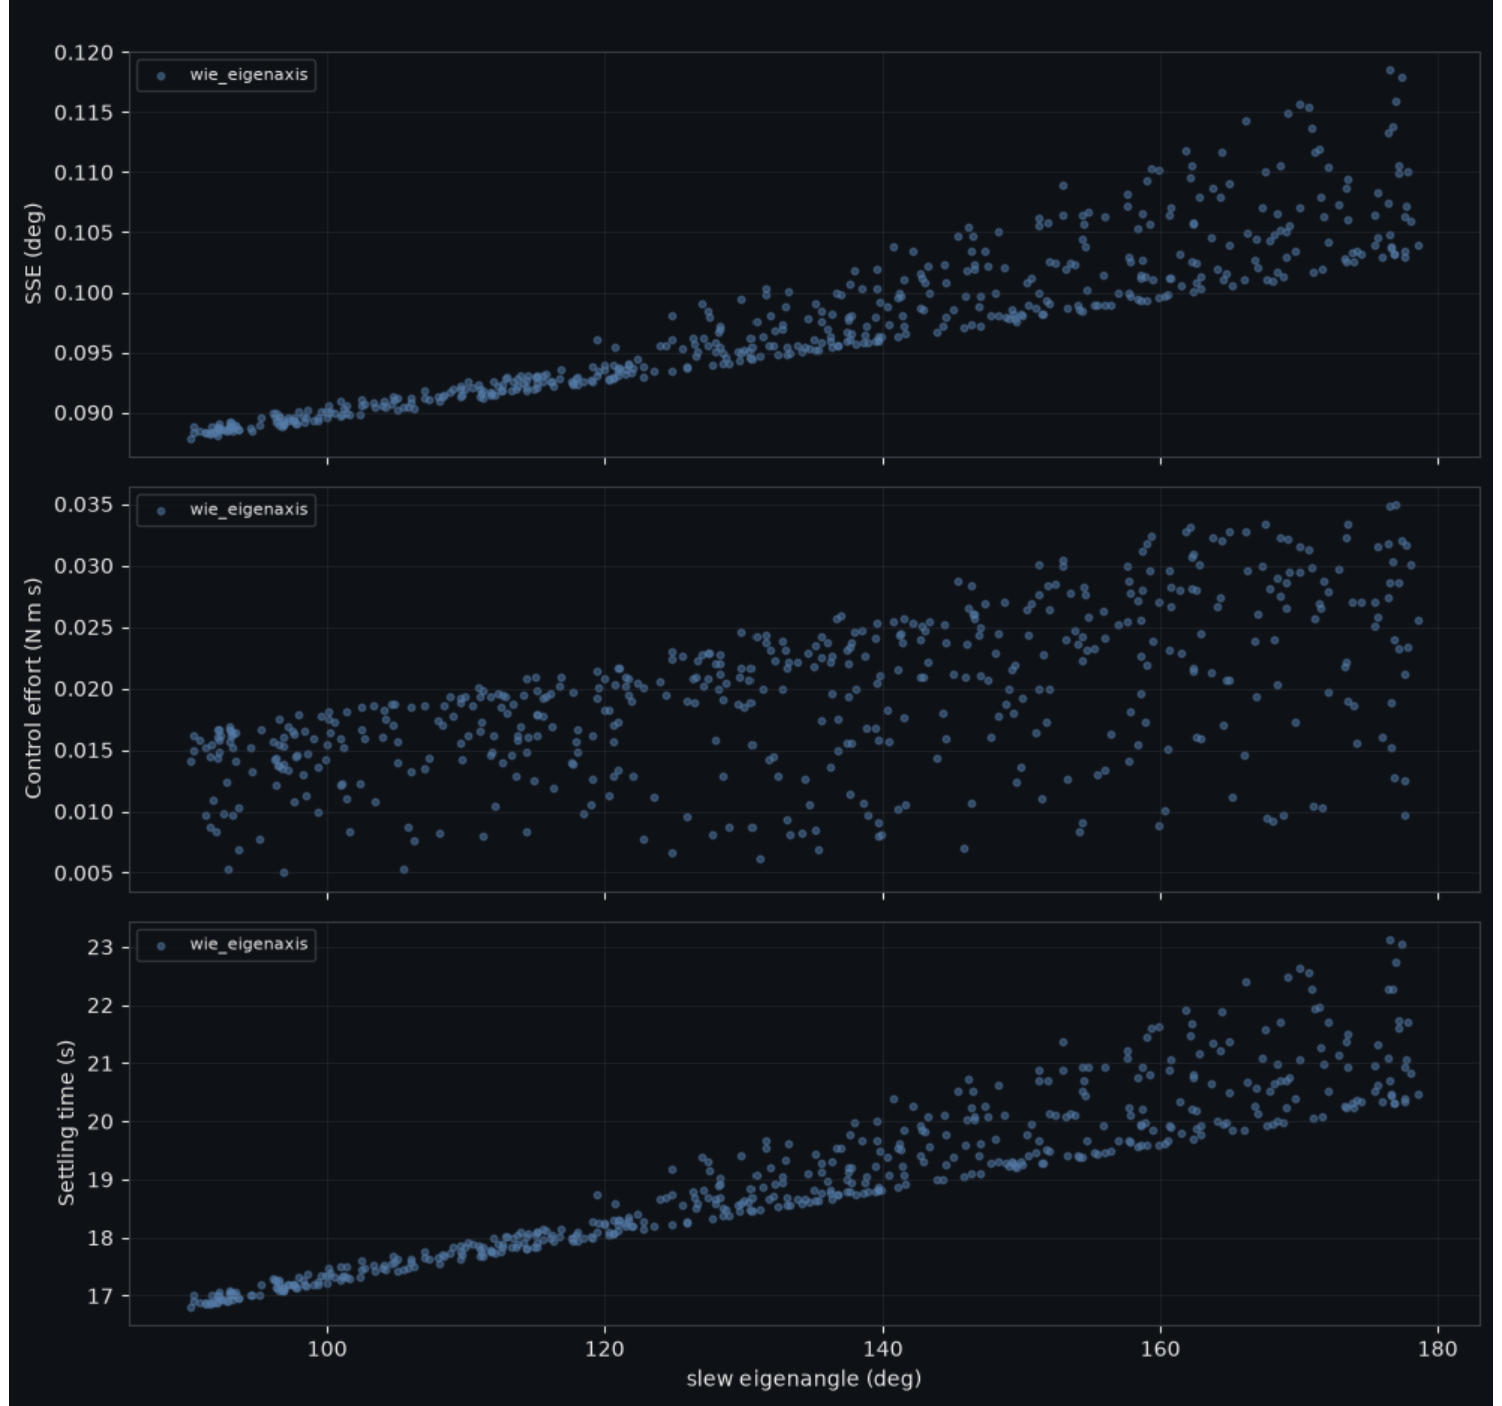
\includegraphics[width=\columnwidth]{figures/simA_montecarlo.png}
\caption{Large-slew campaign (500 trials, $90$--$179^\circ$): steady-state
error, control effort and settling time against slew angle. All three depend
smoothly on the slew angle alone, with a tight spread --- exactly what the
inertia-independent closed loop of \cref{eq:wiecl} predicts, since the response
cannot depend on which axis was drawn.}
\label{fig:montecarlo_A}
\end{figure}

\begin{figure}[!t]
\centering
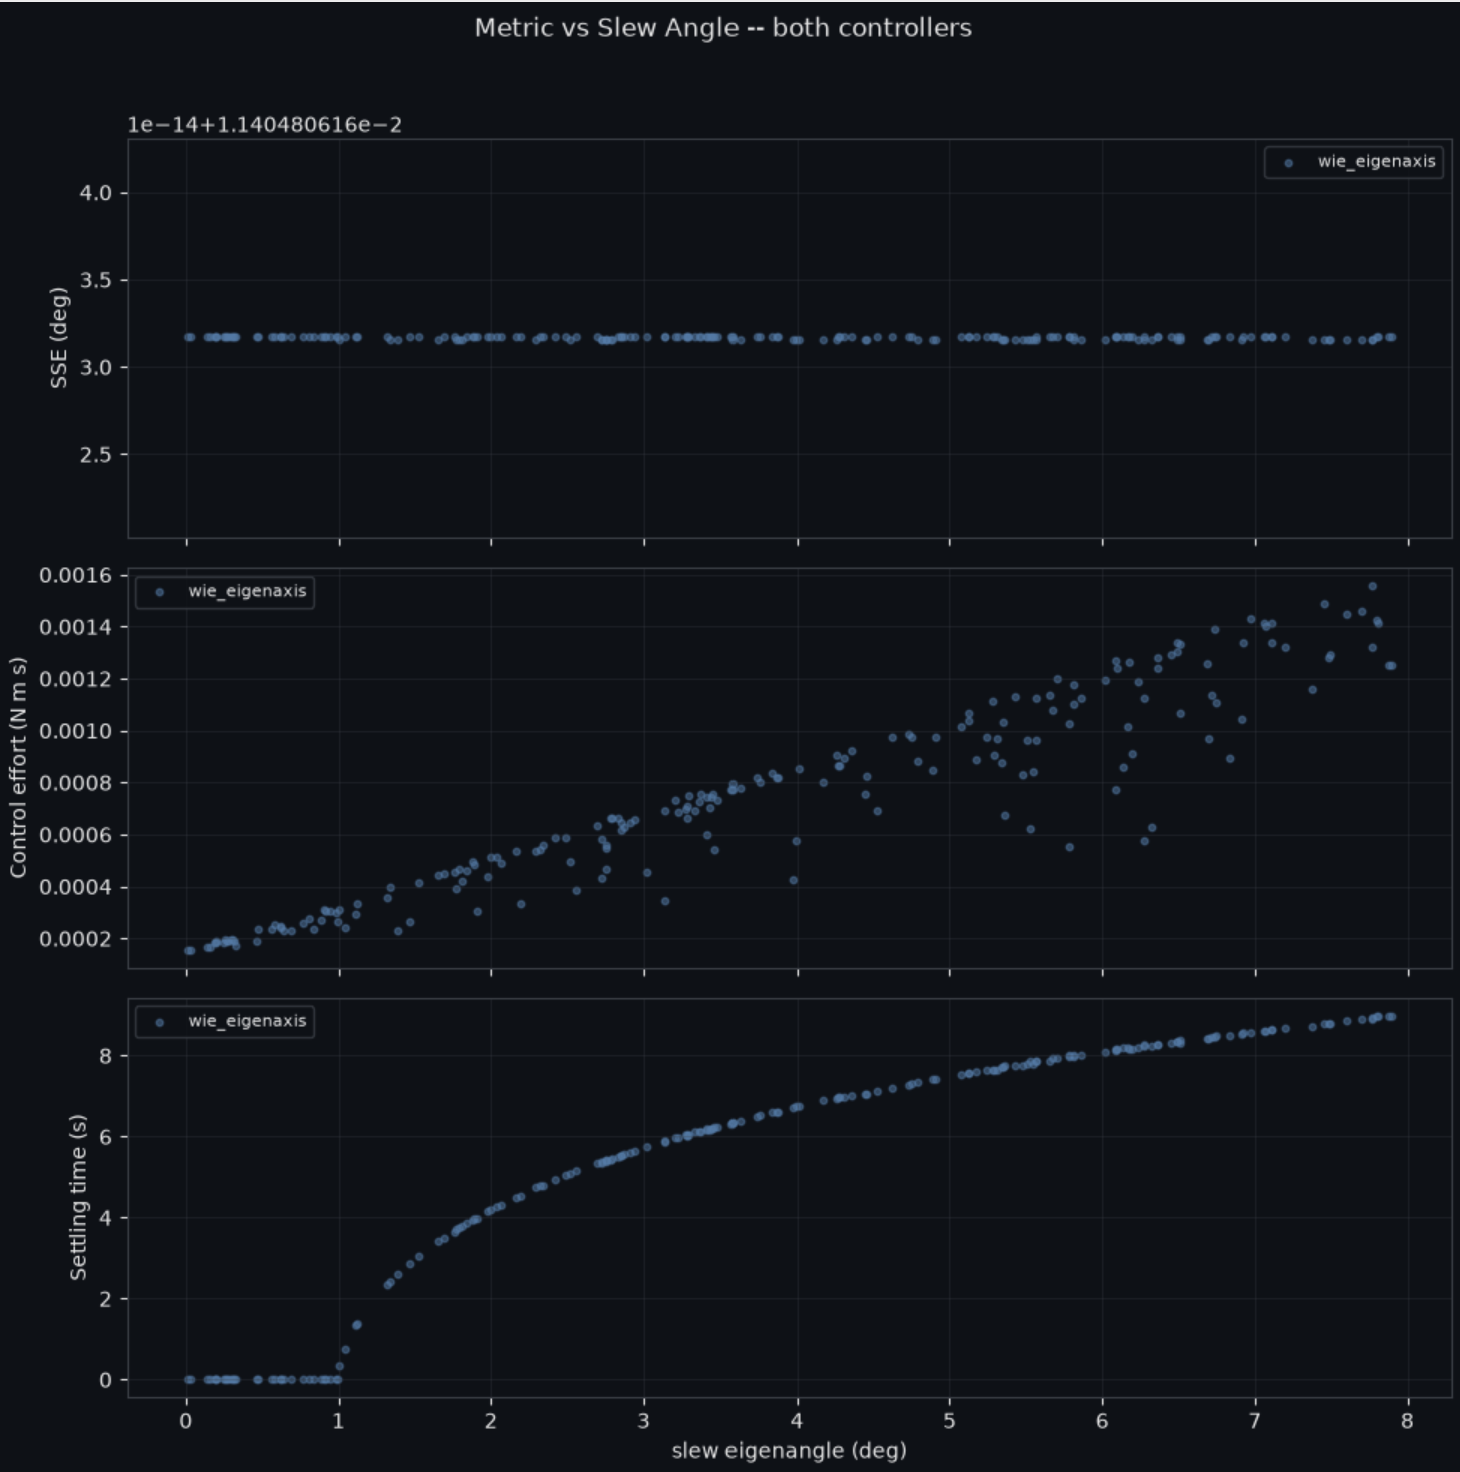
\includegraphics[width=\columnwidth]{figures/simB_montecarlo.png}
\caption{Small-slew campaign ($0$--$8^\circ$, fine-pointing regime): the
steady-state error sits on a flat floor of $\approx0.011^\circ$ set by the
disturbance, independent of slew angle, while settling time and effort scale
smoothly with it.}
\label{fig:montecarlo_B}
\end{figure}

\begin{keybox}[The design generalises, and it beats the baseline on every axis]
Across 500 unseen large slews the Wie regulator settles every one, in
$19.0\pm1.4\unit{s}$, and does so with roughly $19\times$ less control effort,
$5\times$ smaller steady-state error, a tenth the torque saturation and
one-eighth the eigenaxis deviation of the PID baseline (\cref{tab:montecarlo}).
The tight standard deviations are themselves a result: because $\mat{J}$
cancels out of the closed loop, performance depends on the slew \emph{angle}
and not on the axis, so the 500-trial cloud collapses onto a single smooth
curve in \cref{fig:montecarlo_A} rather than scattering.
\end{keybox}

\subsection{Additional results}

\paragraph{Magnetorquer desaturation}
Starting the wheels near their momentum capacity and running the three
magnetorquer rods for $3000\unit{s}$ (half an orbit) reduces stored wheel
momentum by $88\,\%$, from $9.04\times10^{-3}$ to $1.09\times10^{-3}
\unit{N\,m\,s}$, with the attitude error still at $0.000^\circ$ at the end ---
the wheels give up momentum without giving up pointing (R8). The residual
$12\,\%$ is the component of $\vect{h}_w$ parallel to the field, which
\cref{eq:mtqlaw} cannot reach until the field geometry rotates; a full orbit
removes more.
\label{sec:desat_result}

\paragraph{Momentum margin and saturation}
\label{sec:saturation}
Under the true (largely orbit-periodic) gravity gradient the secular momentum
build-up bounds the time to wheel-speed saturation at tens of orbits, so the
desaturation system has ample margin to keep ahead of it. Torque saturation, by
contrast, is transient --- the single $t=0$ clip seen in \cref{fig:scenarioA}(d)
--- and is bounded by the $t_s=30\unit{s}$ sizing; the sign-aware speed limiter
keeps decelerating torque available so a momentarily pinned wheel always
recovers.

\paragraph{Single-wheel failure}
\label{sec:failure}
The three-wheel cone has no spare, but its orthonormal geometry means losing
one wheel removes authority along exactly one inertial direction (the lost
wheel's spin axis) and leaves the orthogonal plane fully actuated --- and
because no wheel axis aligns with a body axis, that is not the loss of roll,
pitch or yaw. A slew whose commanded torque avoids the lost axis executes
unchanged; a general slew loses only the projection onto it.

\paragraph{Power}
The $151.7^\circ$ slew draws well under the $2.0\unit{W}$ ADCS allocation and
costs a negligible fraction of the battery; generation exceeds the margined
load by $1.5\times$. Attitude control is not a power-constrained subsystem on
this spacecraft.

\section{Analysis}
\label{sec:analysis}

\subsection{Requirements compliance}
\label{sec:compliance}

\begin{table*}[!t]
\centering
\caption{Compliance against \cref{tab:requirements}.}
\label{tab:compliance}
\footnotesize
\begin{tabularx}{\textwidth}{@{}llXl@{}}
\toprule
\textbf{ID} & \textbf{Target} & \textbf{Evidence} & \textbf{Status} \\
\midrule
R1 & $\ge85^\circ$ slew          & $151.7^\circ$, \texttt{slew\_160\_40\_30}, \cref{tab:results_slew} & met \\
R2 & $\le40\unit{s}$ settling    & $28.9\unit{s}$ at $152^\circ$, $19.0\unit{s}$ mean over 500 slews, \cref{tab:results_slew,tab:montecarlo} & met \\
R3 & $\le1.0^\circ$ overshoot    & $0.000^\circ$, \cref{tab:results_slew} & met \\
R4 & $\le0.5^\circ$ pointing     & $0.034^\circ$, \cref{tab:results_hold} & met \\
R5 & $\le10^{-3}\unit{deg/s}$    & $2.7\times10^{-5}$, \cref{tab:results_hold} & met \\
R6 & Disturbance rejection       & held at $0.034^\circ$ under bias, \cref{sec:scenarioB} & met \\
R7 & Torque and speed within limits & torque at cap for $0.02\,\%$ of steps; speed $10{,}398$ vs $12{,}000\unit{rpm}$, \cref{tab:results_slew} & met \\
R8 & $\ge50\,\%$ momentum removed per orbit & $88\,\%$ in half an orbit, \cref{sec:desat_result} & met \\
R9 & Momentum conserved to $10^{-12}$ & $4.6\times10^{-15}$ rel., \cref{tab:verification} & met \\
\bottomrule
\end{tabularx}
\end{table*}

All nine targets are met. R7, the actuator-compliance requirement that drove the
$t_s=30\unit{s}$ gain choice, is met with margin: the wheels touch the torque
limit for a single instant at the start of the largest slew ($0.02\,\%$ of the
run) and peak wheel speed sits $13\,\%$ below its limit.

\subsection{Parameter sensitivity}
\label{sec:sensitivity}

\paragraph{Bandwidth} Settling time falls roughly as $1/\omega_n$ while peak
torque rises as $\omega_n^2$, so achievable bandwidth is set by the actuator
rather than by the control design. This is exactly the trade behind the
$t_s=30\unit{s}$ gain choice: a faster design saturates the wheels on a large
slew and loses the eigenaxis property.

\paragraph{Damping} $\zeta=1$ (critical damping) gives no overshoot, which is
what R3 asks for; below $\zeta\approx0.7$ the response overshoots and the wheels
must reverse, costing momentum and time.

\paragraph{Inertia knowledge} This is the design's main exposure, and
\cref{sec:wierobust} is where the paper addresses it. A mismatch leaves an
uncancelled gyroscopic residual proportional to the error, and it also breaks
the $\mat{K}\propto\mat{J}$ tie that the eigenaxis property depends on, so both
the guarantee and the path degrade together. The paper's robust alternative,
$\mat{K}=k\mat{I}$, is implemented as Case~2 and trades the path for
insensitivity to $\Delta\mat{J}$. \texttt{analysis/stability.py}
reports which branch of the Sec.~III proof a given gain set satisfies, so a
mismatched design is flagged rather than assumed safe. \TODO{Run the
inertia-mismatch sweep and report the eigenaxis degradation against mismatch
percentage; \texttt{sim/runner.py} already exposes the hooks that let the
controller and plant carry different tensors.}

\subsection{Physical interpretation}

Two things in the results say something about the real spacecraft rather than
about the simulation.

The transverse axes are the hard ones. With $J_{xx}/J_{zz}=3.55$, a slew about
a transverse axis needs three and a half times the momentum of the same slew
about $z$, so the wheel sizing case is always a transverse manoeuvre. The
elongated 3U geometry is the reason.

The gravity gradient is negligible for pointing and dominant for lifetime. It
sits five orders of magnitude below wheel authority, so it never threatens the
control loop, yet integrated over orbits it is what determines how long the
system runs before needing an external momentum dump. Which of those two facts
matters depends on whether the question is about a manoeuvre or about the
mission.

\subsection{Assumptions and limitations}
\label{sec:limitations}

\begin{itemize}
\item \textbf{Perfect state knowledge.} Attitude determination is out of scope
per the problem statement, so the controller receives true state. The results
are an upper bound on achievable performance, and estimator bandwidth would
become a further constraint on $\omega_n$. This is the largest gap between the
simulation and flight performance.
\item \textbf{Saturation voids the eigenaxis derivation.} \Cref{sec:eigenaxis}
assumes the commanded torque is delivered. Above the bound of
\cref{eq:bwbound} the wheels clip, the delivered torque is no longer
$k\mat{J}\,\delta\vect{q}_v$, and the property degrades --- measured at
$25.95^\circ$ mean deviation on the $152^\circ$ slew. The flown gains satisfy
the stability theorem everywhere, but the eigenaxis claim holds only below the
saturation boundary. Command shaping to keep the demand inside the envelope is
the remedy and is listed in \cref{sec:future}.
\item \textbf{Single rigid body.} Structural flexibility, slosh and
micro-vibration are neglected. This is safe for a 3U whose first structural
mode is far above the control bandwidth, and would not be safe for a
deployable-panel design. The power budget assumes deployable wings, so this
assumption and that budget are in tension and should be revisited together.
\item \textbf{Ideal actuator internals.} Torque and speed limits are enforced,
but motor torque-speed curves, bearing friction, stiction near zero speed and
torque quantisation are not modelled. Friction matters most at zero-speed
crossings, and the cone's invertible allocation leaves no free wheel-speed
direction to bias the wheels away from zero.
\item \textbf{Dipole field model.} The geomagnetic field is a tilted dipole
along a circular orbit, which is adequate for sizing a desaturation actuator
whose job is averaged over orbits, and is not an IGRF-grade model.
\item \textbf{Unverified against a second implementation.} Every check in
\cref{sec:verification} is either a conservation law or an analytical solution
evaluated inside the same codebase. An independent implementation would catch a
shared modelling error that none of them can.
\end{itemize}

%==============================================================================
\section{Challenges}
\label{sec:challenges}

\paragraph{Unwinding from large initial errors}
Early runs starting beyond $180^\circ$ rotated almost a full turn to reach an
attitude that was nearly correct at the start. The behaviour was reproducible
and the controller was clearly stable, which made it look like a tuning problem
for longer than it should have. The cause is the quaternion double cover, and
the fix is the sign latch $s=\sgn[\delta q_0(t_0)]$ of \cref{sec:wie}, applied
consistently in the control law and the integrator state.

\paragraph{Closing the momentum conservation check}
The conservation test failed by a small persistent amount until the
$\vect{\omega}\times\vect{h}_w$ term was restored to \cref{eq:dynamics}. This
is the clearest argument for undoing the omission: a verification test that
always fails slightly gets ignored, and then it stops catching anything.

\paragraph{Two parameter sources that disagreed}
The inertia tensor lived in both \texttt{constants.py} and a base YAML file,
and the two drifted apart, ending up with different values. Every downstream
number depended on which one a given script happened to read. The fix was to
delete the YAML and build the base configuration layer from the constants
module, so there is one place to change the spacecraft.

\paragraph{One gain candidate consumed an entire tuning budget}
A single candidate in the NSGA-II search took $1800\unit{s}$ to simulate
against a $3\unit{s}$ baseline, without raising an exception. Because results
are collected in submission order, it blocked its whole generation and consumed
the wall-clock budget, finishing two generations of one seed instead of the
planned run. The fix was a per-candidate timeout that scores an over-running
candidate worst-case rather than waiting for it.

\paragraph{The wheel array changed after the CAD was built}
The mid-evaluation's four-wheel pyramid was a real mechanical design with a
packaging trade behind it. The simulation has since moved to a three-wheel cone
whose cant angle is fixed by orthogonality, so that trade no longer exists, and
what replaces it is the open CAD mismatch of \cref{sec:cad}. \TODO{Ask Tulika
what changed mechanically in the bracket and mounting plate for three wheels
rather than four, and what the switch cost or saved.}

%==============================================================================
\section{Conclusion and Future Work}
\label{sec:conclusion}

A reaction wheel attitude control system for a 3U CubeSat has been designed,
implemented from first principles and verified against conservation laws and
analytical solutions. The control law is the Wie quaternion feedback regulator,
chosen for its eigenaxis property and sized to stay inside the actuator
envelope.

The flown design slews $151.7^\circ$ to $1^\circ$ in $28.9\unit{s}$ with no
overshoot, $0.0005^\circ$ final error and $0.00^\circ$ mean eigenaxis
deviation, touching the wheel torque limit for only $0.02\,\%$ of the run. It
holds an $8.5^\circ$ recovery at $0.034^\circ$ steady state under a disturbance
five orders of magnitude above the true gravity gradient. Across 500 unseen
random large slews it settles every one in $19.0\pm1.4\unit{s}$, using roughly
$19\times$ less control effort and holding the eigenaxis eight times tighter
than a settling-time-tuned PID baseline. Magnetorquer desaturation removes
$88\,\%$ of stored wheel momentum in half an orbit without loss of pointing,
and total angular momentum is conserved to $1.7\times10^{-17}$ relative.

All nine requirements are met. The one deliberate trade is settling speed:
sizing for $t_s=30\unit{s}$ rather than something faster is what keeps even the
largest slew unsaturated and eigenaxis-true, and the Monte-Carlo campaign shows
the resulting design generalises well beyond the two mandated scenarios.

The most transferable result is methodological: a conservation law catches what
a response plot cannot. The angular momentum check found errors that looked
entirely plausible on a plot of the attitude, and it is three lines of code.

\subsection{Future work}
\label{sec:future}

\begin{enumerate}
\item \textbf{An independent implementation} of the plant, in Simulink or any
other environment, to catch shared modelling errors that internal consistency
checks cannot.
\item \textbf{Attitude estimation}, most naturally a multiplicative extended
Kalman filter on the quaternion error, removing the perfect-state assumption
that currently bounds the results from above.
\item \textbf{LQR}, currently a stub in \texttt{control/lqr.py}, giving an
optimality baseline for the effort figures in \cref{tab:montecarlo}.
\item \textbf{Nadir pointing against a rotating reference}, which needs the
$\vect{\omega}\times\vect{\omega}_r$ transport term in the error rate.
\item \textbf{Actuator detail}: torque-speed curves, bearing friction and
quantisation, the assumptions most likely to change the saturation results.
\item \textbf{Random-vibration (PSD) qualification and full-assembly modal
analysis}, beyond the single-bracket quasi-static and modal check of
\cref{sec:cad_fea}.
\end{enumerate}

%------------------------------------------------------------------------------
\section*{Contribution Statement}

\TODO{State who did what; evaluators ask in the viva. Suggested wording, adjust
to reality: V.S.\ developed the simulation architecture, the dynamics and
kinematics modules, the control laws and their stability analysis, the gain
search, and the verification campaign. T.C.\ developed the CAD assembly, the
wheel and bracket design, material selection and mass budget, and the
mass-properties extraction feeding \cref{eq:inertia}.}

%------------------------------------------------------------------------------
\begin{thebibliography}{99}

\bibitem{wie1989}
B.~Wie, H.~Weiss, and A.~Arapostathis, ``Quaternion feedback regulator for
spacecraft eigenaxis rotations,'' \emph{J.\ Guid.\ Control Dyn.}, vol.~12,
no.~3, pp.~375--380, 1989.

\bibitem{mortensen1968}
R.~E. Mortensen, ``On systems for automatic control of the rotation of a
rigid body,'' Electronics Research Laboratory, Univ. of California,
Berkeley, Rep.~63-23, 1963.

\bibitem{wiebarba1985}
B.~Wie and P.~M.~Barba, ``Quaternion feedback for spacecraft large angle
maneuvers,'' \emph{J.\ Guid.\ Control Dyn.}, vol.~8, no.~3, pp.~360--365, 1985.

\bibitem{markley}
F.~L.~Markley and J.~L.~Crassidis, \emph{Fundamentals of Spacecraft Attitude
Determination and Control}. New York: Springer, 2014.

\bibitem{deb2002}
K.~Deb, A.~Pratap, S.~Agarwal, and T.~Meyarivan, ``A fast and elitist
multiobjective genetic algorithm: NSGA-II,'' \emph{IEEE Trans.\ Evol.\
Comput.}, vol.~6, no.~2, pp.~182--197, 2002.

\bibitem{shirazi2014}
A.~Shirazi and M.~Mirshams, ``Pyramidal reaction wheel arrangement optimization
of satellite attitude control subsystem for minimizing power consumption,''
\emph{Int.\ J.\ Aeronaut.\ Space Sci.}, vol.~15, no.~2, pp.~190--198, 2014.

\bibitem{schaub}
H.~Schaub and J.~L.~Junkins, \emph{Analytical Mechanics of Space Systems},
4th~ed. Reston, VA: AIAA Education Series, 2018.

\bibitem{wertz}
J.~R.~Wertz, Ed., \emph{Spacecraft Attitude Determination and Control}.
Dordrecht: Kluwer Academic, 1978.

\bibitem{sidi}
M.~J.~Sidi, \emph{Spacecraft Dynamics and Control: A Practical Engineering
Approach}. Cambridge, U.K.: Cambridge Univ.\ Press, 1997.

\bibitem{khalil}
H.~K.~Khalil, \emph{Nonlinear Systems}, 3rd~ed. Upper Saddle River, NJ:
Prentice Hall, 2002.

\bibitem{ogata}
K.~Ogata, \emph{Modern Control Engineering}. Pearson.

\bibitem{cds}
\emph{CubeSat Design Specification (CDS)}, The CubeSat Program, Cal Poly SLO.

\bibitem{maxon}
maxon motor ag, ``ECX FLAT 22 L brushless DC motor datasheet.''
\TODO{add URL and accessed date}

\end{thebibliography}

%==============================================================================
\appendices

\section{Nomenclature}
\label{app:nomenclature}

\begin{table}[!h]
\centering
\footnotesize
\begin{tabularx}{\columnwidth}{@{}lX@{}}
\toprule
\textbf{Symbol} & \textbf{Meaning} \\
\midrule
$\vect{q},q_0,\vect{q}_v$ & Attitude quaternion, scalar and vector parts \\
$\delta\vect{q}$        & Error quaternion, \cref{eq:qerr} \\
$\vect{\omega}$         & Body rate relative to $\FI$, resolved in $\FB$ \\
$\mat{J}$               & Total inertia about the CoM, wheels locked \\
$\mat{R}(\vect{q})$     & Body-to-inertial rotation matrix \\
$\mat{A}$               & Wheel distribution matrix, \cref{eq:Amatrix} \\
$\vect{\Omega}$         & Per-wheel speeds \\
$\vect{h}_w$            & Net wheel momentum in body axes \\
$\vect{\tau}_s$         & Per-wheel axial torques \\
$\vect{\tau}_\text{cmd}$& Commanded body torque \\
$\vect{\tau}_w$         & Torque actually delivered to the body \\
$\vect{\tau}_d$         & External disturbance torque \\
$\theta,\phi_i$         & Wheel cant angle from $+z$, azimuth angles \\
$k,d$                   & Wie gain scalars, $\mat{K}=k\mat{J}$, $\mat{D}=d\mat{J}$ \\
$\mat{K},\mat{D},\mu$   & Wie regulator gains and decoupling factor \\
$k,d$                   & Wie scale factors, $\mat{K}=k\mat{J}$, $\mat{D}=d\mat{J}$ \\
$\vect{m},\vect{B}$     & Magnetorquer dipole and geomagnetic field \\
$\omega_n,\zeta$        & Design natural frequency and damping ratio \\
$\Delta t$              & Integration step \\
$\skewm{\vect{a}}$      & Skew-symmetric cross-product matrix \\
$\mat{A}\pinv$          & Moore--Penrose pseudo-inverse \\
\bottomrule
\end{tabularx}
\end{table}

\section{Derived Quantities}
\label{app:derived}

All values follow from the cone geometry of \cref{eq:Amatrix_num} with
$\theta=54.7356^\circ$, $\tau_\text{max}=4.0\times10^{-3}\unit{N\,m}$ and
$h_\text{max}=7.288\times10^{-3}\unit{N\,m\,s}$.

\begin{table}[!h]
\centering
\footnotesize
\begin{tabular}{@{}llr@{}}
\toprule
\textbf{Quantity} & \textbf{Expression} & \textbf{Value} \\
\midrule
Orthonormality check & $\mat{A}\T\mat{A}-\mat{I}$        & $<10^{-6}$ \\
Torque, $x$          & $\sqrt{2}\,\tau_\text{max}$        & $5.657{\times}10^{-3}$ \\
Torque, $y$          & $2\sin\theta\,\tau_\text{max}$     & $6.532{\times}10^{-3}$ \\
Torque, $z$          & $3\cos\theta\,\tau_\text{max}$     & $6.928{\times}10^{-3}$ \\
Momentum, $x$        & $\sqrt{2}\,h_\text{max}$           & $1.031{\times}10^{-2}$ \\
Momentum, $y$        & $2\sin\theta\,h_\text{max}$        & $1.190{\times}10^{-2}$ \\
Momentum, $z$        & $3\cos\theta\,h_\text{max}$        & $1.262{\times}10^{-2}$ \\
Inertia ratio        & $J_{xx}/J_{zz}$                    & $3.548$ \\
Asymmetry factor, $y$& $\sqrt{J_{xx}/J_{yy}}$             & $1.022$ \\
Asymmetry factor, $z$& $\sqrt{J_{xx}/J_{zz}}$             & $1.883$ \\
Bandwidth bound      & $\min_j\sqrt{u_{\max,j}/(J_{jj}\theta_0)}$ & $0.316\unit{rad/s}$ \\
Gravity gradient     & $\tfrac{3}{2}n^2|\Delta J|$        & $4.76{\times}10^{-8}$ \\
Saturation time      & $H_{\max,x}/\tau_\text{gg}$        & $2.17{\times}10^{5}\unit{s}$ \\
Magnetorquer torque  & $m_\text{max}B_0$                  & $6.24{\times}10^{-6}$ \\
Solar generation     & orbit average                      & $8.5\unit{W}$ \\
\bottomrule
\end{tabular}
\end{table}

\section{Repository and Reproduction}
\label{app:repo}

Source: \url{https://github.com/vivekswamy18092007/Reaction-wheel-attitude-control}.
\TODO{Tag the commit used for every result in this report and record the tag
here.}

\begin{lstlisting}[caption={Repository layout.},captionpos=b]
src/deimos/       the package (Table VIII)
configs/
  scenarios/      6 manoeuvre presets
  controllers/    Wie gain presets (all four paper cases, plus the
                  manoeuvre/hold integral-action pair)
studies/          Jupyter notebooks: manual tuning,
                  power analysis, Monte Carlo analysis
tests/            159-case verification suite
runs/             command output, gitignored
overnight_tune.py NSGA-II gain search driver
monte_carlo_verify.py  randomised campaign driver
legacy/           pre-package scripts
\end{lstlisting}

Reproducing a single result, the verification suite, and a gain search:

\begin{lstlisting}
deimos run --scenario configs/scenarios/slew_55_65_15.yaml \
           --controller configs/controllers/wie_eigenaxis.yaml

python -m pytest tests/ -q

python overnight_tune.py --type WIE --hours 8
\end{lstlisting}

\end{document}
